%%%%%%%%%%%%%%%%%%%%%%%%%%%%%%%%%%%%%%%%%%%%%%%%%%%%%%%%%%%%%%%%%%%%%%%%%%%%%%%
%% Developers' guide                                                         %%
%%%%%%%%%%%%%%%%%%%%%%%%%%%%%%%%%%%%%%%%%%%%%%%%%%%%%%%%%%%%%%%%%%%%%%%%%%%%%%%
\chapter{Developers' guide}
\label{chap:developers-guide}

In this chapter, we discuss how to extend the ePNK, with new functionality and
applications, with new Petri net types, with new graphical appearances, or with
new tool specific extensions. For all these extensions, the ePNK provides
\emph{extension points} so that the extensions can be made without changing
the actual code of the ePNK\footnote
 {Technically, you would not even need to see the code of the ePNK, but
  looking at it might help understanding the ideas and principles behind the
  ePNK.}%
. Actually, the ePNK does not even provide own extension points for adding
functionality: The existing Eclipse extension points are good enough for
that for now.

This chapter addresses developers, who want to develop extensions for the ePNK,
and it gives a systematic overview over the concepts of the ePNK by discussing
different examples for the different concepts. This chapter is organized along
the different concepts for extending the ePNK and for using its API. In
contrast, Chapter~\ref{chap:tutorial} is organized along a single running
example, which covers the most relevant concepts and goes through the
conceptual steps as well as through the technical details. Both chapters
are written in such a way that they can be read independently of each other.

Section~\ref{sec:adding-functions} shows how to add some functionality to the
ePNK, which could be a model checker, or some other analysis or verification
function for Petri nets, or which could be a function that reads a net in PNML
and produces some net in some other format, or a function that generates a net
that is stored in PNML format. Section~\ref{subsec:developer:applications}
shows how to implement \emph{applications}%
  \index{ePNK!Application|DEF}
that visualize the results on top of the graphical editor of the ePNK and can
also interact with the end user while they are running.

Section~\ref{sec:adding-types} shows how to add new Petri net types
to the ePNK. Simple net types can almost completely be generated from a
model; for more complex Petri net types, such as high-level Petri nets, a
mapping to XML must be defined and parsers need to  be implemented.

Section~\ref{sec:dev:graphical} shows how to customize the graphical
appearance of some features of some types of Petri nets.

Section~\ref{sec:adding-toolspecific-info} shows how to add tool specific
information to the ePNK.

At last, Sect.~\ref{sec:overviewAPI} gives an overview of the projects of the
ePNK and Sect.~\ref{sec:developer:deploy} briefly discusses how to deploy own
extensions.

All of these extensions are discussed by the help of some examples,
which are deployed together with the ePNK. In these examples,
we assume that the reader is familiar with the main principles and ideas
of Eclipse, its plug-in architecture, and Eclipse plug-in development.
We cannot give a detailed introduction to Eclipse and to Eclipse
plug-in development here (when you have the feeling that you need more
background on these issues, the ``Platform Plug-in Developer Guide'' which is part of Eclipse
might be a good starting point: ``Help'' $\rightarrow$ ``Help contents''; and there
are many other Eclipse resources \cite{Eclipse-WWW,ClRu08}).
Still, Sect.~\ref{sec:development-environment} gives a brief overview
of Eclipse plug-in development.
We go a bit more into the details for EMF and explain some of the steps that
need to be done in EMF more explicitly, but it is also recommended to read
up on some details on EMF \cite{BSM06} before starting with own development
projects. 

In order to use the ePNK for implementing own extensions, developers would
need some understanding of the PNML core model and the API generated from
it. Therefore, Sect.~\ref{sec:ePNK-PNMLCoreModel} gives a brief introduction
to the PNML core model as it is used in the ePNK and discusses some differences
to the PNML core model from ISO/IEC 15909-2. 

\section{Eclipse: A development platform for the ePNK}
\label{sec:development-environment}

As briefly discussed in Sect.~\ref{sec:Eclipse-IDE} already, Eclipse is
an Integrated Development Environment (IDE).% 
  \index{Eclipse!IDE}
Here, we briefly explain how to set up the Eclipse environment so that you can
work on your own extensions and have a look into the code of the
examples, which are discussed in chapter. For a hands-on experience, you
should install Eclipse and the ePNK as explained in Chapter~\ref{chap:install}.

\subsection{Importing ePNK projects to the workspace}
\label{sec:dev:import-ePNK}

As a developer, you would probably want to have a look into some parts of
the source code of the ePNK. Therefore, the ePNK is deployed in such a way
that you can easily import the relevant ePNK plug-in projects to your
workspace with all their source code and all their models, so that you
can inspect the code and the models from which major parts of the code
were generated. Furthermore, the source code of all ePNK projects is
available on GitHub: \url{https://github.com/ekkart/ePNK}

Here, we explain how to import the ePNK projects into your Eclipse development
workspace as source projects -- assuming that you have installed the ePNK
in your Eclipse already. Initially, it is recommended to import
only the basic project {\tt org.pnml.tools.epnk} into the workspace;
later during this developers' guide, we will mention several other
projects that might be interesting for you to have a look at. In
the end, Sect.~\ref{sec:overviewAPI} gives an overview of important
ePNK projects and their main function and purpose.

In order to import an ePNK project (or any other plug-in project which
is running behind the scenes in your Eclipse), you first need to open the Eclipse
\emph{Plug-ins view}.%
  \index{Eclipse!Plug-ins view|DEF}
To this end, in the Eclipse workbench, select ``Window'' $\rightarrow$ ``Show
view''  $\rightarrow$ ``Other...''; then select ``Plug-ins'' from the
category ``Plug-in Development''. Typically, this view would also open
when you switch to the \emph{Plug-in Development perspective}%
  \index{Eclipse!Plug-in Development perspective|DEF}
of Eclipse.
Once the Plug-ins view is open, browse this view and find the ePNK
plug-in {\tt org.pnml.tools.epnk}. Right-click on this plug-in and
select ``Import As'' $\rightarrow$ ``Source Project''. After that,
you will find the project  {\tt org.pnml.tools.epnk} in the Eclipse
package explorer or some other open resource browser.

In this project, you can see the source code in the folder ``src'' and
also the model files in the folder ``model''. But, if you did not install some extra tools
yet, you will not be able to open these models with some
reasonable editor. Section~\ref{subsec:installingEcoreTools}
briefly discusses which additional tools you need to install to your version
of Eclipse so that you are able to inspect -- and later create -- 
these kind of models and diagram files.

You can import all ePNK projects to the workbench as discussed above,
but only some few projects will be relevant for you. This chapter
introduces you to the most relevant ones -- one after an other
(in the end, Sect.~\ref{sec:overviewAPI} gives an overview of the ePNK
 projects).
If you, eventually, are confident in developing functions and applications
for the ePNK, you might also want to contribute to the ePNK and
make your extensions and changes to the ePNK plug-ins. In that case,
you can ask to be given access to the ePNK development repository.  

\index{Eclipse!Development workbench|(DEF}%
\index{Eclipse!Runtime workbench|(DEF}%
In your workbench, you have now the project {\tt org.pnml.tools.epnk}, 
which is the basis for developing new plug-ins and, in particular, extensions to
the ePNK. We start calling this workbench \emph{development workbench} now.
The reason for introducing an additional adjective to the term \emph{workbench}
here is that you need to start another workbench from this one, in order
to start Eclipse with the new extensions that you are developing in
the development workbench. This additional instance of Eclipse is called
the \emph{runtime workbench} since this is where the ePNK with your new
extensions is running. It will very much look like the original ePNK as discussed in
Chapter~\ref{chap:users-guide} -- just with the extensions from your
development workbench also running.  The
runtime workbench can be started from the development workbench by 
``Run'' $\rightarrow$ ``Run Configurations...'' and then selecting ``Eclipse
Application'' and pressing the ``New'' icon and then ``Run''. After you have
started the development workbench in this way once, it will be enough to press
the ``Run'' button in the tool bar for starting the runtime workbench again. 
For now, however, we do not start the runtime workbench since we need to
implement some new functionality first.%
  \index{Eclipse!Development workbench|)}%
  \index{Eclipse!Runtime workbench|)}

\subsection{Installing the EMF and Ecore Tools SDK}
\label{subsec:installingEcoreTools}

As mentioned already, a major part of defining a new Petri net type is creating
an Ecore model which captures the concepts of the new Petri net type; most of
the code can then be generated from such a model. In order to be able to do
that, you need to install the \emph{Eclipse Modeling Tools} (\emph{EMT}) in
your Eclipse or install the \emph{Eclipse Modeling Tools} package as your version
of your Eclipse.

The details are discussed in Chapter~\ref{chap:install}. Note that most of
the diagrams associated with the Ecore models were created with version 1 of
Ecore Tools and have not been updated to version 2 of Ecore Tools yet. These
diagrams are not supported by Eclipse newer than Luna. But, if you install
the feature for legacy Ecore diagrams as discussed in Chapter~\ref{chap:install},
you will be able to open them. It is, however, strongly recommended that
new models and diagrams are created with the current version of Ecore Tools,
since the legacy Ecore Diagram Editor eventually might not work any more for
future versions of Eclipse. 

You can check if you have installed Eclipse and its EMT extensions correctly:
Open the project {\tt org.pnml.tools.epnk} and, in that project, open the folder
{\tt model}. The files with extensions ``.ecore'', ``.ecorediag'', and ``.genmodel''
should have special icons. And when you double-click on ``.ecore'' and
``.genmodel'' files, a tree-editor should open on them. When you double-click
on ``PNMLCoreModel.ecorediag'', you should see an Ecore model in a class diagram
like graphical notation as shown in Fig.~\ref{fig:ePNK-IDE}. 

\begin{figure}[hbt!!]
  \centerline{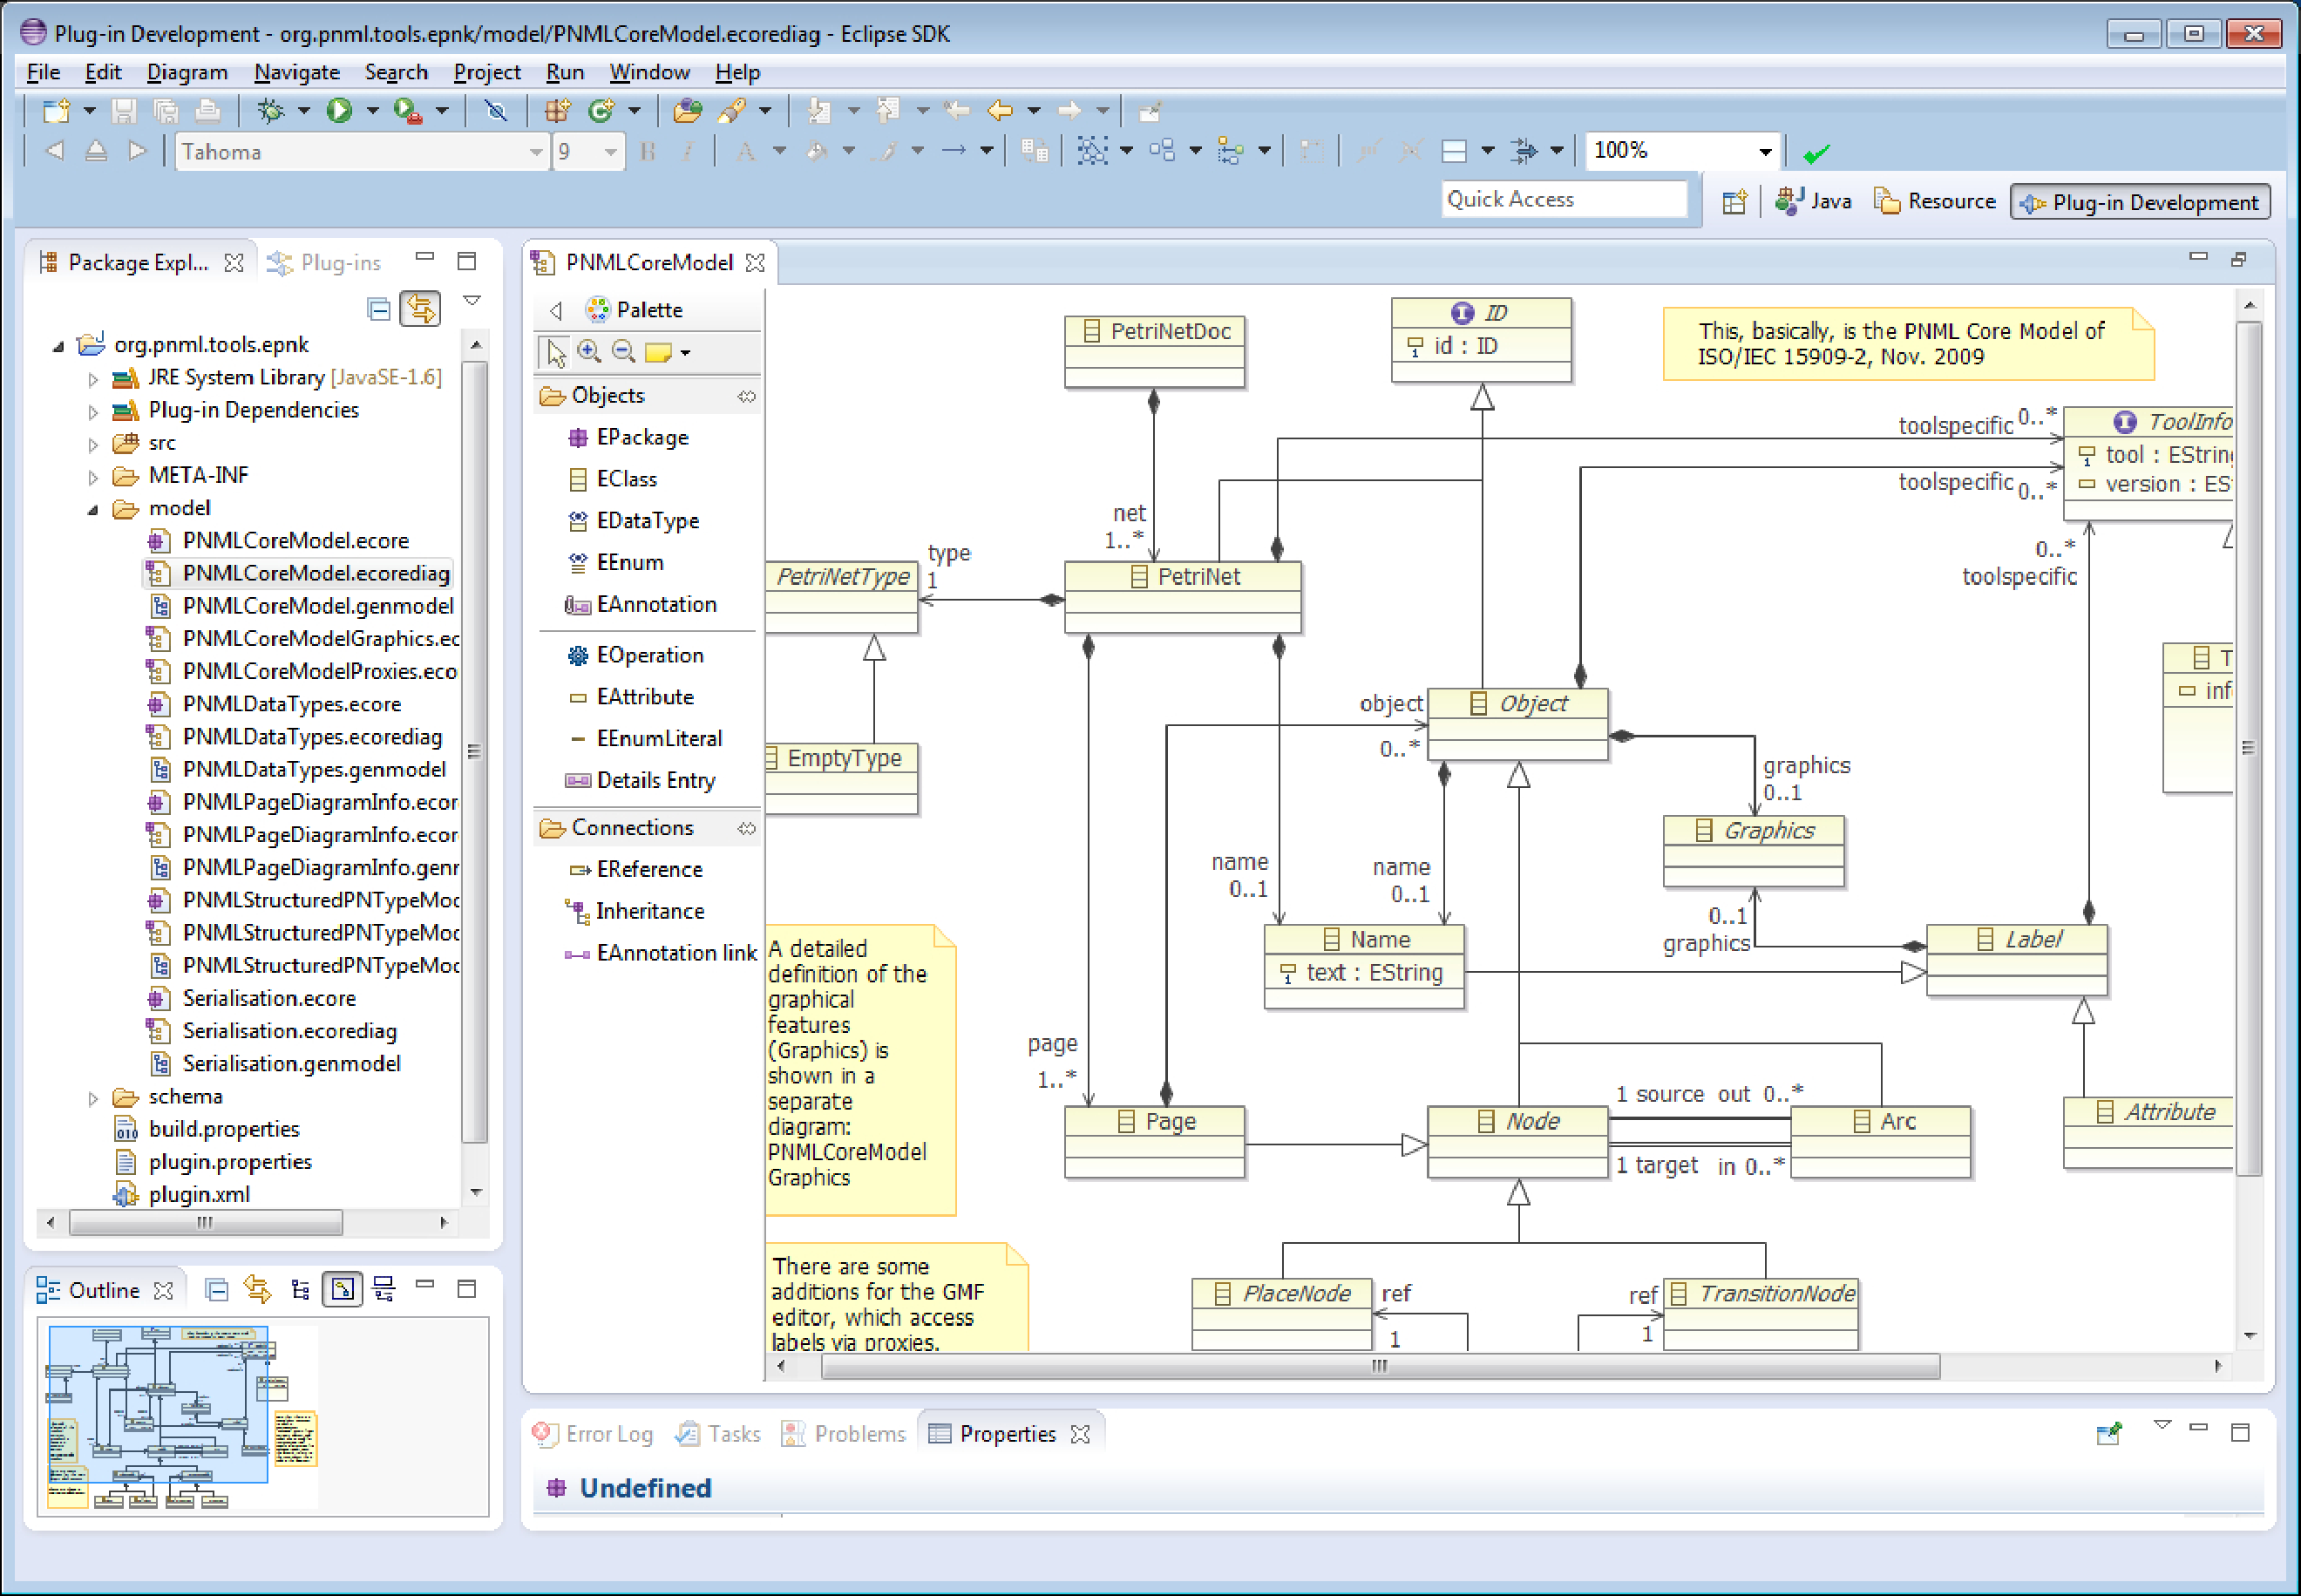
\includegraphics[scale=.28]{ePNK-IDE}}
  \caption{Developer's view with the ePNK PNML core model}
  \label{fig:ePNK-IDE}
\end{figure}


\section{The PNML core model in the ePNK}
\label{sec:ePNK-PNMLCoreModel}
% \index{PNML core model|(DEF}
\index{ePNK!PNML core model|(DEF}

For using the ePNK as a developer it is important to have a more
detailed understanding of the \emph{PNML core model} since the API
for accessing, navigating and modifying Petri nets is generated
from this model.  In Sect.~\ref{subsec:installingEcoreTools}, you have seen
already were to find and how to open the diagrams of the PNML core model
and some related diagrams. And when you start developing with the
ePNK, you will probably need to have a look into these diagrams
once in a while, in order to understand the details of the relation
between the different classes and concepts of PNML. 

In this section, we give an overview of the PNML core model of the
ePNK and discuss some of the differences to the PNML core model
of ISO/IEC~15909-2. As discussed in Sect.~\ref{subsec:PNMLcoremodel} already,
the PNML core model of the ePNK is slightly more general than the one of
ISO/IEC~15909-2:2011 \cite{ISO-IEC:15909-2-2011} (see Fig~\ref{fig:MetaModel}).
One of the main differences is the following: According to ISO/IEC~15909-2,
a page is not considered to be a node; in the ePNK, a page is considered to be
a node. This way, it is possible to define Petri net types in the ePNK that
allow arcs to be connected to pages (e.\,g.\ in order to define a Petri net
type that mimics substitution transitions of CPNs \cite{JeKr09}). Keeping
this in mind, might be particularly important, when defining the
constraints for arcs of net types (such as the ones for P/T-nets as
defined in Sect.~\ref{subsubsec:simplePNTDconstraints}), when you do
not want to allow to connect pages to other nodes with arcs.

The other differences of the PNML core model are a bit more technical
and will be discussed below. You might want to have a look at
Fig.~\ref{fig:MetaModel} of the PNML core model of ISO/IEC 15909-2:2011 
and at Fig.~\ref{fig:ePNK-IDE}, while we discuss the difference. For
more details, you can also open the Ecore diagrams in the project
{\tt org.pnml.tools.epnk} in your Eclipse workspace, provided you
have installed the legacy Ecore Diagram editor.

Most importantly, the {\tt type} of a Petri net is an attribute
of the class {\tt PetriNet} according to ISO/IEC~15909-2, whereas, in the
ePNK, it is a composition to a class that must inherit from the abstract class
{\tt PetriNetType}.%
  \index{ePNK!PetriNetType@{\tt PetriNetType}}
Instances of this class represent the Petri net type and will provide some
services to the ePNK to generically maintain the features of the respective
Petri net type. This is discussed in more detail in
Sect.~\ref{sec:adding-types}.
The PNML core model of the ePNK also provides one concrete class for a Petri net
type, which does not exists in ISO/IEC~15909-2:2011: {\tt EmptyType},%
  \index{ePNK!EmptyType@{\tt EmptyType}}
which represents a Petri net without any labels other than {\tt Names}.

In the ePNK, the {\tt source} and {\tt target} reference of the class
{\tt Arc} have a corresponding opposite reference from the {\sf Node} to its
{\tt out}-going and {\tt in}-coming {\tt Arc}s. These opposite references
are not serialized to the XML document, however, since this would not be
compliant with the PNML format. The opposite references will, however,
be restored when loading the Petri net. These opposite references are very
convenient when navigating between different elements of the net.

In turn, the ePNK does not have the class {\tt Annotation}%
  \index{ePNK!Annotation|DEF}
of ISO/IEC~15909-2, which represents those \emph{labels}%
  \index{Label|DEF}
that should be shown as graphical annotations
of the respective node or arc in the graphical editor. There exists a
class {\tt Attribute},%
  \index{ePNK!Attribute|DEF}
however, which represents those labels that
should be represented as properties of the respective element only,
but not as annotation in the graphical editor\footnote
 {By plugging in some graphical extensions, attributes can still have an effect
  on the graphical appearance of a Petri net.}%
. In the ePNK, all \emph{labels}%
  \index{ePNK!Label|DEF}
that are not attributes are considered to be
annotations. This has historical reasons, since the first version of the
ePNK did not support attributes at all; but, it also avoids making mistakes
in Petri net type definitions: it is impossible to define labels
that are neither attributes nor annotations.

At last, the PNML core model of the ePNK defines a separate interface {\tt ID},%
  \index{ePNK!ID|DEF}
which is used to unify all those elements that need a unique identifier in a
PNML document. All classes that must have such an identifier, implement the
interface {\tt ID} in the PNML core model of the ePNK. The reason for adding
the class {\tt ID} to the ePNK PNML core model is that, this way, the ePNK can
handle elements with an identifier in a uniform way; with the separate
id attribute for all elements as defined in the PNML core model of
ISO/IEC~15909-2, this would require much more effort.%
  \index{ePNK!PNML core model|)}%
% \index{PNML core model|)}
  
The attentive reader might also have noticed that the PNML core model of the
ePNK does not contain any OCL constraints, whereas the PNML core model
of ISO/IEC 15909-2 does. This, however, does not mean that the ePNK ignores
these constraints; in the ePNK, constraints are just added in a different way:
they are plugged in on top of the model. We will see examples of
how ePNK constraints are plugged in to the ePNK resp.\ to Eclipse later
(e.\,g.\ in Sect.~\ref{subsubsec:simplePNTDconstraints}).

\section{Adding functions}  
\label{sec:adding-functions}
\index{ePNK!Function|(DEF}

Next, we discuss how new functionality can be added to the ePNK. As discussed
earlier, there are two different ways of new adding new functionality to the
ePNK: \emph{Functions} take some net, possibly some user input, do some computing
and then report a result -- typically via some dialog window. After that, the function
is over and done with. The model checker from
Sect.~\ref{subsec:user:model-checker} is a typical example of a function.
By contrast, \emph{applications}%
  \index{ePNK!Application|DEF}
are started on a net; then, they show some feedback on top of the graphical
editor, the user can interact with the application, and the visual feedback
will be updated accordingly. Typically, an application finishes only
when the user explicitly terminates it. The simulator for high-level nets
of Sect.~\ref{subsec:user:hlpng-simulator} is a typical example
of an application.

In this section we, discuss the implementation of functions for the
ePNK. Basically, we use the standard mechanism of Eclipse to plug in
and start functions -- as \emph{views},%
  \index{Eclipse!View}
\emph{wizards},%
  \index{Eclipse!Wizard} 
\emph{actions},%
  \index{Eclipse!Action}
\emph{command handlers},%
  \index{Eclipse!Command handler}
\emph{jobs}%
  \index{Eclipse!Job}
or \emph{dialogs}.%
  \index{Eclipse!Dialog} 
In this manual, we explain the use of these concepts on the side, as far as they
are necessary. Since setting up jobs in a proper way can sometimes be a bit
tedious, the ePNK provides some utility classes that make programming jobs a
bit easier.

The focus of this section is on the use of the API of the ePNK that is
generated from the PNML core model and the Petri net type definitions
by the \emph{Eclipse Modeling Framework} (\emph{EMF}).%
  \index{EMF}
On the side, we point out some of the general principles of EMF and some
practical issues on working with EMF. For a more detailed introduction
to EMF, we refer to \cite{BSM06}. In this section, we do not only show
how to access, navigate and manipulate nets; we discuss also how
to open, create and write PNML files programmatically.

To this end, this section discusses how to plug in functionality into
the ePNK (or to Eclipse in general) in three different ways.
\begin{itemize}
\item Section~\ref{subsec:file-overview} shows how to implement a new
Eclipse view, which gives an overview of a PNML file that is selected in one of
the Eclipse resource explorer views. This section will also discuss how
top open and access the contents of a PNML file.

\item Section~\ref{subsect:multi-agent} shows how to implement a \emph{wizard}
for creating a PNML file (actually, the coded is based on a wizard that was
automatically created by the Eclipse ``new plug-in project wizard'').
This wizard creates a PNML file with a P/T-System that represents
a simple mutual exclusion algorithm for a number of agents -- where the
number can be selected by the user in one of the dialogs of the wizard.
The Petri net is split up to different pages, so that the Petri net for each
agent is contained in a separate page. In particular, we will discuss how
to create a PNML file, how to fill it with some contents and how to save it.

\item Section~\ref{subsec:tutorial-MC} shows how to implement a
simple pop-up menu on a selected Petri net (in the tree editor), which
starts a model checker, asking the user for some formulas to be checked,
and then checking the formulas on the net. Since model checking can take
quite some time, the model checker will run in the background and can
be aborted by the user. This uses Eclipse's concept of jobs. On the side, this
shows how to use some of Eclipse's user dialog functions.
\end{itemize}

In the end, Sect.~\ref{subsec:devloper:functitions:utilities} gives an overview
of the different functions of the ePNK (and the API generated from its EMF
model), some hints on how to work with this API in Eclipse and in EMF
general, as well as some additional ePNK utilities and helper classes that make it more
convenient to handle and access some of the information stored in a PNML document.
Experienced Eclipse and EMF developers, might want to start reading the overview
in Sect.~\ref{subsec:devloper:functitions:utilities} first, and come back
to Sect.~\ref{subsec:file-overview}--\ref{subsec:tutorial-MC} for some details
later.

\subsection{Accessing a PNML file and its contents: A file overview}
\label{subsec:file-overview}
\index{Eclipse!View|(DEF}

In this section, we discuss how to implement a new (and very simple)
Eclipse \emph{view}, that will give an overview of the contents of a PNML
file that is selected in the explorer. Figure~\ref{fig:file-overview-view} shows
a screenshot of the result. For the selected file ``hlpng-gmf.pnml''
in the ``Project Explorer'',  the ``ePNK File Overview'' at the
bottom left shows that the selected file is a Petri net document,
which contains 3 Petri nets, a high-level net, a P/T-net, and
an empty net; the type of a net is represented by its unique
URI. The name of the first net is ``A high-level next
example''; the other two nets do not have a name.

\begin{figure}[hbt!!]
  \centerline{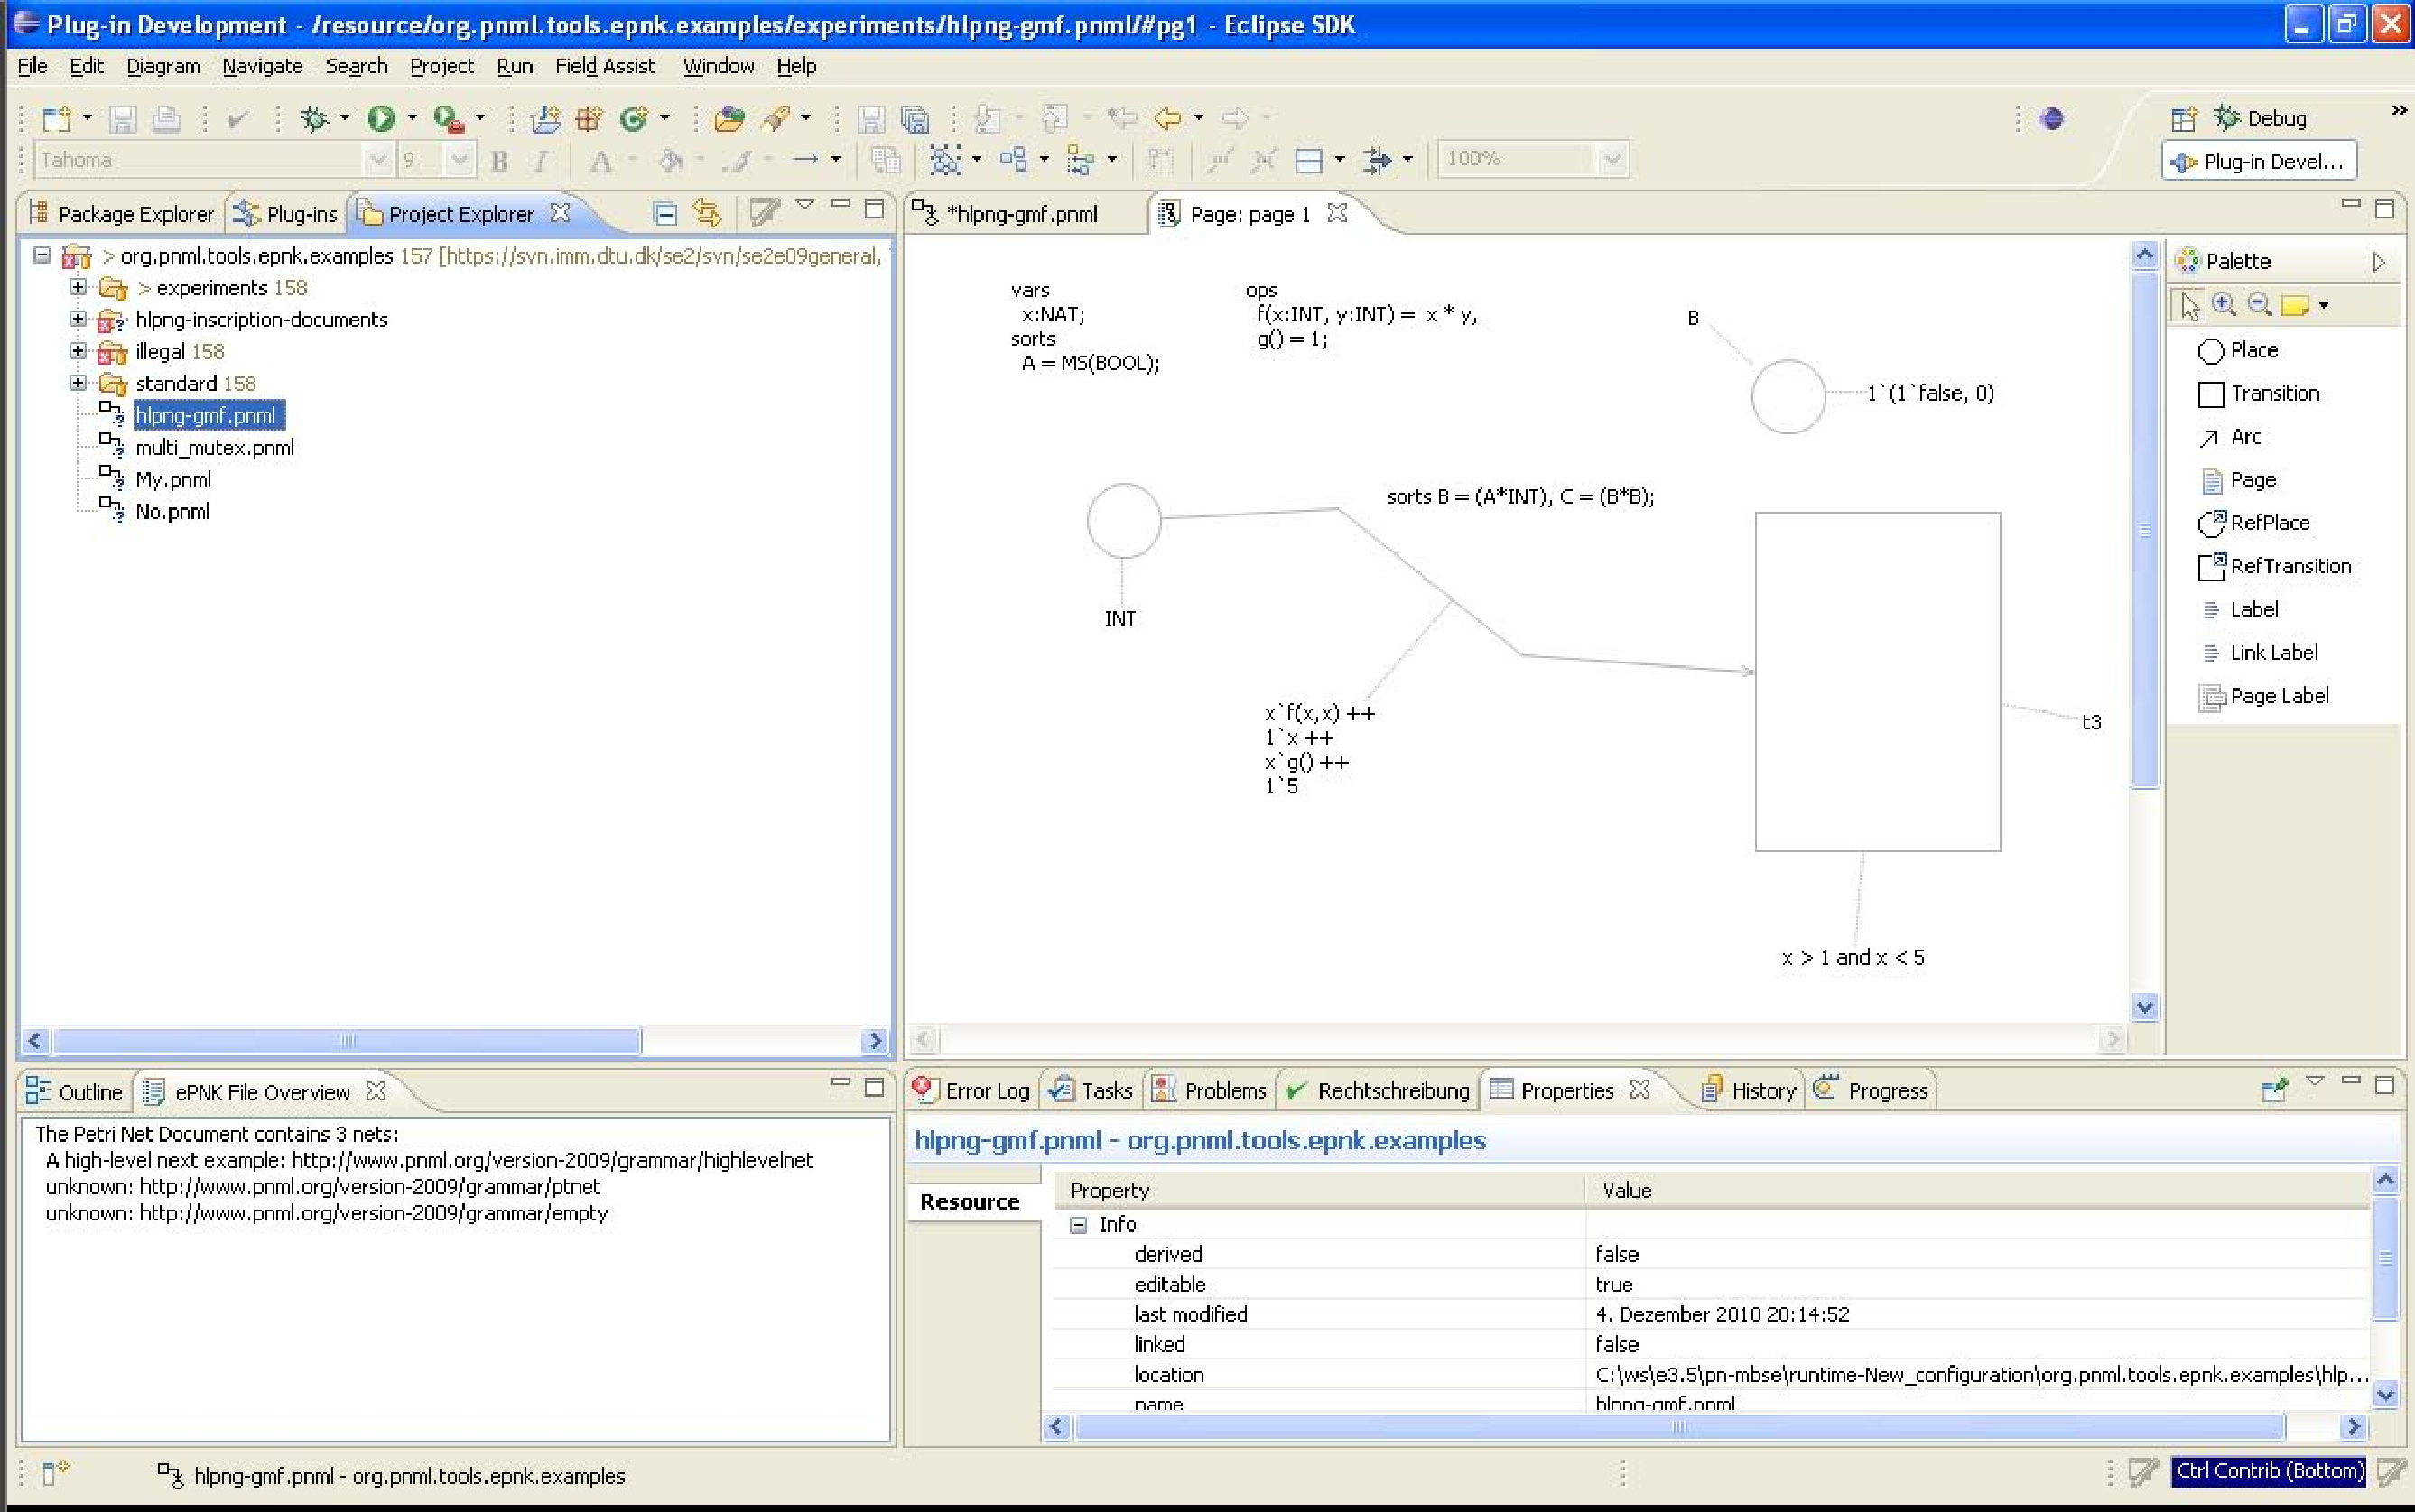
\includegraphics[scale=.27]{OverviewView}}
  \caption{The ePNK with the ``File Overview'' view}
  \label{fig:file-overview-view}
\end{figure}

This view and its functionality is implemented in the plug-in project
{\tt org.pnml.tools.epnk.functions.tutorial}. We go through this
project now\footnote
 {Remember that you can import the source code of that project to your
  development workspace from the ``Plug-ins'' view by selecting the
  project, right-clicking on it and then choosing ``Import As'' $\rightarrow$
  ``Source Project'' (see Sect.~\ref{sec:dev:import-ePNK}.}%
.  In addition to the overview view discussed above, this project also contains
the implementation of the wizard for creating a PNML document which will be
discussed later in Sect.~\ref{subsect:multi-agent}.

The implementation of the view is contained in a single Java class: {\tt
PNMLFileOverviewView} in the package
{\tt org\qnsep{}pnml\qnsep{}tools\qnsep{}epnk\qnsep{}functions\qnsep{}tutorial\qnsep{}overviewview}.
We briefly explain the general structure of this view class, an extract
of which is shown in Listing~\ref{lst:overview1};
%
\begin{figure}[htbp!]
\lstinputlisting[label=lst:overview1,tabsize=2,stringstyle=\small,%
caption={Class {\tt PNMLFileOverviewView}: Infrastructure}]%
  {code/PNMLFileOverviewView1.java}
\end{figure}
%
we deleted all imports, an attribute definition, and all comments; if needed
this information can be looked up in the source code. The class extends the Eclipse
{\tt ViewPart},%
  \index{Eclipse!ViewPart@{\tt ViewPart}|DEF}
which actually makes it an Eclipse view, and it implements the {\tt
ISelectionListener},%
  \index{Eclipse!ISelectionListener@{\tt ISelectionListener}|DEF}
which allows our view to obtain the information on the object that the user
has currently selected in the workbench.
Note that this class does not have an explicit constructor. The reason is that
the view will be set up via the {\tt createPartControl()} method:
In the first three lines of that method, a viewer (which represents the content
of that view) is initialized, and so-called providers will enable the view to
properly show the contents. Since these are standard Eclipse providers, we do
not discuss the details here.
In the last two lines of the {\tt createPartControl()} method,
our viewer registers itself with the Eclipse selection mechanism
as a \emph{selection listener}%
  \index{Eclipse!Selection listener}
and then creates the information that should be shown for the current user selection
by calling the {\tt selectionChanged()} method for the current selection. We will discuss
the respective method {\tt selectionChanged()} below.  Note that
there are two other methods. The {\tt setFocus()} methods forwards the
focus properly to the content of the view, once the view is focused.
More important is the {\tt dispose()} method: the implementation of
this method makes sure that our view removes itself as a selection
listener once it is disposed (which typically would happen when the
user decides to close the view).

Once the view has registered itself as a selection listener with
the Eclipse workbench, its {\tt selectionChanged()} method is
called whenever there is a change in the user's selection.
In the implementation of this method, the kind of the current
selection is analysed and it is checked whether the first
selected element is a file (i.\,e.\ whether it implements the
interface {\tt IFile}). If so, the method {\tt getOverviewInfo()}
for accessing the actual contents of the file and for computing
the contents of the overview is called; this produces an array of
Strings, which then will be set as the new contents of that view --
and, this way, shown to the user.%
\index{Eclipse!View|)}

The {\tt getOverviewInfo()} method is probably the most interesting
part here, since it shows how to open and access a PNML or a
PNX file (we do not even need to make a difference here). The implementation
of this method is shown in Listing~\ref{lst:overview2}.
%
\begin{figure}[htbp!]
\lstinputlisting[label=lst:overview2,%
tabsize=2,stringstyle=\small,%
caption={Class {\tt PNMLFileOverviewView}: Accessing the file}]%
  {code/PNMLFileOverviewView2.java}
\end{figure}
% 
Up to line 7, it is checked whether the file extension is
either ``pnml'' or ``pnx'' (the two file extensions, the ePNK uses
for storing Petri net files -- ``pnml'' represents files in PNML format, and
``pnx'' represents Petri net files in XMI, which we call PNX); then, the
path to that file is extracted and a URI of that path is created.
Actually, Eclipse provides also user dialogs and file dialogs that would
allow us to ask the user for a file name that would be returned as a URI; here
we used the selection mechanism and the file to get hold of some legal URI
of a PNML or PNX file. Therefore, the code that comes now, could be used at any
other point when a program wants to read and access some file, once we have a
String with the path to the file: This starts with creating a \emph{resource
set}%
  \index{Eclipse!Resource set|DEF}
and, within that resource set creating a \emph{resource}%
  \index{Eclipse!Resource|DEF}
with the given URI, which is the first parameter of the {\tt getResource()}%
  \index{EMF!getResource@{\tt getResource()}|DEF}
method; the second parameter indicates whether cross-references to other resources should be
resolved lazily or not (which is not relevant here). Note that, in EMF, a
resource or file should always be accessed (and created, see
Sect.~\ref{subsect:multi-agent} for more information) via a
resource set. After we successfully got the resource, we can obtain its contents
by the {\tt getContents()}%
  \index{EMF!getContents@{\tt getContents()}|DEF}
method which returns a list of its top-level objects
-- in case of PNML, this list should contain exactly one {\tt PetriNetDoc} object. 
Being defensive, we check whether the contents exists and whether its first element is an instance
of {\tt PetriNetDoc}. If so, we go systematically through all the contained nets, get
their names and their PNML types and add a String with that information to the
String array with the result. In the other cases, we return some error
messages. Note that we do not need to close the file, or do anything else after
we have obtained the information we need.

Let us have a closer look at how the contents of the Petri net
document is accessed, once we have obtained a {\tt PetriNetDoc}
object. For any reference and attribute of the \emph{PNML core model},%
  \index{PNML core model}
the ePNK API%
  \index{ePNK!API|DEF}
has corresponding \emph{getter}%
  \index{EMF!getter method|DEF}
 and \emph{setter methods}.%
  \index{EMF!setter method|DEF}
For example, if a class has an attribute {\tt name} of type {\tt String}, the
{\tt getName()} method will return the {\tt String} with that name, and with
{\tt setName()} we could set it -- but we do not change the net in this example.
For attributes and features with a multiplicity greater than one, this is
slightly different. For example, a {\tt PetriNetDoc} object can contain many nets;
therefore, {\tt getNet()} will return a list of nets, which we then can
iterate over to obtain the individual nets. And by adding a net
to this list, this Petri net would be added to the Petri net
document (see \ref{subsect:multi-agent} for examples).

As stated above, class {\tt PNMLFileOverviewView}
implements the ``ePNK File Overview'' as we have seen it in
Fig.~\ref{fig:file-overview-view}. But, it is not enough to just implement
this class; it would not show up in Eclipse, because Eclipse would
not know that it exists. In order to make the view known to
Eclipse, we need to define it as an \emph{extension}:%
  \index{Eclipse!Extension|DEF}
This is done in the project's ``plugin.xml''%
  \index{Eclipse!pluginxml@{\tt plugin.xml}|DEF}
file. Double clicking on the
``plugin.xml'' file, will give you a convenient editor for defining and	editing
the extensions you want to define. Explaining the actual extensions is a bit
easier with the XML fragment that is produced by this editor. The
fragment relevant for our overview view is shown in Listing~\ref{lst:overview-plugin}.
%
\begin{figure}[htbp!]
\lstinputlisting[language=XML,label=lst:overview-plugin,tabsize=2,stringstyle=\small,%
caption={Defining the overview view extension in ``plugin.xml''}]%
  {code/overview-plugin.xml}
\end{figure}
% 
It says that we contribute our \emph{extension}%
  \index{Eclipse!Extension|DEF}
to the Eclipse \emph{extension point}%
  \index{Eclipse!Extension point|DEF}
{\tt org.eclipse.ui.views}, which is a
new Eclipse view. The category defines where and under which category
the new view can be found, when the user wants to open it
via the Eclipse ``Show View'' menu.
We define a category specifically for the ePNK and then define the actual view
referring to this category.
The attributes of the view say that a view of this kind can
at most be open once, that it uses the above category, and refer to the
class which actually implements it: {\tt PNMLFileOverviewView};
and the attributes define an icon (used in the tab of that view) and 
a name for that view.

Note that in order to access some of the classes such as {\tt Resource},
{\tt Resource\optsep{}Set}, and some of the ePNK classes like {\tt PetriNetDoc},
{\tt PetriNet}, etc.\ in the implementation of the view, we would also need to
define dependencies to the plug-in projects by which they are provided: If you
open the file ``plugin.xml'', you will find these projects in the tab ``Dependencies''.  But
this is a more technical issue, which we do not go into the details.

Now, you could start the runtime workbench of Eclipse; from there, you could open the
``ePNK File Overview'' by ``Window''$\rightarrow$ ``Show
View''$\rightarrow$ ``Other...'' and then selecting ``ePNK File Overview''
in the category ``ePNK''. This will show the view in the workspace as shown
in Fig.~\ref{fig:file-overview-view}. Whenever the user selects some
PNML or PNX file in the package explorer, this view will show an overview
of the contents of the selected file. Since this plug-in project is deployed
with the ePNK 1.0.0 already, it is of course not even necessary to start the
runtime workbench -- the view is already there in the development workbench,
once the ePNK is installed.


\subsection{Writing PNML files: Generating multi-agent mutex}
\label{subsect:multi-agent}

Next, we discuss how to create new PNML files and how to fill them
with some contents.
In typical applications, the contents might come from a file in a format of
another Petri net tool, which should be converted to PNML. In our example,
however, we programmatically generate a Petri net: my favourite semaphore mutex
example, which was used in Sect.~\ref{subsec:user:model-checker} as an
example for model checking already.
To make things slightly more interesting, the number of agents competing for the
semaphore is a parameter.  This function is implemented as an Eclipse
\emph{wizard}%
  \index{Eclipse!Wizard|DEF}
and it was implemented by creating a new file wizard for PNML files
automatically by the Eclipse ``New Plug Project'' wizard choosing the
``custom plug-in wizard'' with the choice of the ``New File Wizard'' in
the ``Template Selection'' dialog. But, this does not need to bother you too
much. If you are interested in the manual changes made to the automatically
generated code, you will find all the manual changes in the two classes
in the package {\tt org.pnml.tools.epnk.functions.tutorials.wizards} enclosed
by comments like {\tt // eki: ... }. These packages are contained in the
same plug-in project, 
{\tt org.pnml.tools.epnk.functions.tutorials},
as discussed in Sect.~\ref{subsec:file-overview} already.

In the rest of this section, we focus on the explanation of the parts of the
implementation that are concerned with the creation of the file and its contets.
This functionality is implemented in the method {\tt createPNMLFile()} of
the class {\tt MultiAgentMutexNetWizard}, which is shown in
List.~\ref{lst:createFile}. The parameter {\tt path} is a String representation
of a path to the file that should be created. The parameter {\tt number} is the
number of agents that should be created in the mutex net that will be generated.  

Creating the Petri net programmatically is quite straightforward, but code
intensive. Therefore, we have split up the creation process into several parts
for the different elements, which will be discussed top-down from creating
the document, the net, its pages, and the places, transitions, reference
places, and arcs on them. We discuss these methods one after the other --
and omit some boring ones in the end (you can find all details in the
source code).
%
\begin{figure}[bp!] % [htbp!]
\lstinputlisting[label=lst:createFile,tabsize=2,stringstyle=\small,%
caption={Method {\tt createPNMLFile(String path, int number)}}]%
  {code/MultiAgentMutexNetWizard1.java}
\end{figure}
%
Listing~\ref{lst:createFile} shows the method that creates the
file: First, it calls the method {\tt createPetriNetDoc()} that creates the
Petri net document, which is discussed later. This is the contents of the file
that we want to write. Then, we convert the path into a URI. Then, we create a
resource set%
  \index{Eclipse!Resource set|DEF}
-- from which the resource (the file) is create. Surprisingly
enough, this is already all we need to do. At this point, we can add the
contents to the resource. Note that it does not even matter whether the
resource is a PNML file or a PNX file -- Eclipse will, dependent on the file
extension, chose the right implementation of the resource so that either a PNML
file or a PNX file is written once we save the resource in the end. But, we
configured the wizard in such a way that the user can chose only
the ``pnml'' extension.

Adding the contents follows the same principle that we have discussed already.
With {\tt getContents()}%
  \index{EMF!getContents@{\tt getContents}|DEF}
we get a list of EMF objects (which would be empty,
since the resource was newly created right now); then we add the Petri net
document to this list. The only thing left is to save the resource, which is
done by calling the {\tt save()}%
  \index{EMF!save@{\tt save()}|DEF}
method. Note that the save method has a
parameter, that could be used to configure the way a file is saved. 
But, {\tt null} is fine here -- and you should only change this, if you know
exactly what you are doing.

\index{ePNK!API|(DEF}%
Let us dive a bit deeper into the method {\tt createPetriNetDoc()}, which
takes one parameter only -- the number of agents.
%
\begin{figure}[htbp!]
\lstinputlisting[label=lst:createFile2,tabsize=2,stringstyle=\small,%
caption={Method {\tt createPetriNetDoc(int number)}}]%
  {code/MultiAgentMutexNetWizard2.java}
\end{figure}
%
This method is shown in Listing~\ref{lst:createFile2}. In the
second line, a new Petri net document is created. Note that this is not done
using Java's {\tt new} construct. Rather, the \emph{factory}%
  \index{EMF!Factory|DEF}
for the PNML core model is obtained by
{\tt Pnmlcoremodel\optsep{}Factory\qnsep{}eINSTANCE},%
  \index{ePNK!PnmlcoremodelFactory@{\tt PnmlcoremodelFactory}|DEF}
which is then used for creating a new {\tt PetriNeyDoc} object. It is part of the
EMF philosophy that clients using the generated code should not know anything about
the actual implementation of classes. And EMF strongly recommends to create
new objects only via these factories.
Note that also the new net is not directly created; it is created by
using the ePNK's type registry {\tt PetriNetTypeExtensions},%
  \index{ePNK!PetriNetTypeExtensions@{\tt PetriNetTypeExtensions}|DEF}
  \index{ePNK!Type registry|DEF}
which creates the Petri net with the correct type from its URI. Note that the
net will be {\tt null}, if no net type is registered for the respective URI.

After creating the net, its id is set by the {\tt setId()} method. Note that this
could be any string, but it is our responsibility to make sure that all ids
are different (if we chose to create the ids programmatically). Then, the net is
added to the list of nets of that document: to this end, we get
the list of all nets of the document via the {\tt getNet()} method on which we
call the {\tt add()} method. There is no way to directly add a net to
a document. 

After that, a name label is created, its text value is set, and the
name label is added to the net. 

Next, a new page is created by calling a separate method, which is added
to the list of pages of the net, and the place semaphore is created
as the single object on this page. To this end, we use the
{\tt createPlace()} method. 

In the for-loop at the end of the method, for each agent, there
will be created one page with the net for each agent.

All the other methods follow the same principles, and there  is
not too much interesting to see in them.
%
\begin{figure}[htbp!]
\lstinputlisting[label=lst:createFile3,tabsize=2,stringstyle=\small,%
caption={Method {\tt createAgentPage()}}]%
  {code/MultiAgentMutexNetWizard3.java}
\end{figure}
% 
Therefore, we finish with discussing the method {\tt  createAgentPage()},
which is shown in Listing~\ref{lst:createFile3}. This method
creates 3 places, one reference place (referring to the semaphore
that was created on the first page above), 3 transitions, and 8 arcs.
What makes this method a bit more interesting is the graphical
information that is added to the arcs: some intermediate point,
which makes the net look a bit nicer. If you have a closer look
at the {\tt createTransition()}, {\tt createPlace()}, and  {\tt createRefPlace()}
you will find similar constructs for defining the position and size
of the nodes, and the position of the labels associated with them.
But this is straightforward and follows the exact principles
of ISO/IEC~15909-2 (see \cite{HKea09}). Note that, if a reference
pace is created, the place it refers to needs to be set by
{\tt setRef()}; therefore, we need to pass the the place {\tt semaphor}
to the {\tt createRefPlace()} method as a parameter.

Once the implementation
of the wizard class is finished, it must be made know to Eclipse: it must be
plugged in via the ``plugin.xml''. But, we do not discuss this here since
this is similar to plugging in a view (have a look
into the ``plugin.xml'', if you are interested).

In the runtime workbench (or a version of the ePNK in which this plug-in
is installed already), you could invoke this function as follows: Go to the
resource explorer -- or any other explorer -- of the workbench, press
the right mouse button and select ``New''$\rightarrow$``Other...'',
select ``Multi-agent Mutex Net Wizard'' in the category ``ePNK''. Then,
a dialog opens in which you can choose a folder\footnote
  {If you have selected exactly one folder when you invoke the
   wizard, the fields of this dialog will be pre-set.}
(``container'') in which this file should be created, a ``file name'' (which
must have extension ``pnml''), and the number of agents. Note that, normally,
the file creation wizard would overwrite existing files. This ``multi-agent''
wizard, however, was modified in such a way that existing files won't be
overwritten accidentally.%
  \index{ePNK!API|)}

\subsection{Long-running functions: A model checker}
\label{subsec:tutorial-MC}
\index{Job|(DEF}

In this section, we discuss the implementation of a model checker for P/T-Nets,
which, actually, are interpreted as EN-Systems here. The model-checker is based
on a simple library for symbolic model checking that was developed for
teaching purposes: \emph{Model Checking in Education} (\emph{MCiE})\footnote{
see \url{http://www2.cs.uni-paderborn.de/cs/kindler/Lehre/MCiE/}}. This MCiE
library is deployed as part of the ePNK tutorials.

In this developers' guide, we will not go into the details of model checking
and its theoretical foundation, since this is not the point of this tutorial
at all. For more information on model checking, we refer to a standard text book
on model checking~\cite{CGP99}. The point of this tutorial is to show how some
function can be installed as a \emph{pop-up} menu with an \emph{action} on a
Petri net that is open in the tree editor\footnote
  {Note the extension points for pop-up menus and actions are deprecated
   since Eclipse~4.2. But, they still work -- eventually, this will be adjusted
   by using Eclipse commands and handlers.}%
. Model checking can actually be quite computation intensive and
could take quite some time; therefore, we need to make sure that the actual
model checking action does not block the graphical user interface of Eclipse
while the model checker is running. Eclipse provides \emph{jobs} for this
purpose, which allow to run tasks (or jobs) in the background.
The ePNK provides some convenience classes that make it a bit easier to set up
and start jobs, which are running in the background -- and provide a possibility
to show a result in a dialog, once the job is finished.

The model checking functionality is implemented in the plug-in project
{\tt org\qnsep{}pnml\qnsep{}epnk\qnsep{}functions\qnsep{}modelchecking}. Like the other projects,
you can import the source code of this project to your workspace via
the Eclipse ``Plug-ins'' view and the ``Import As'' $\rightarrow$ ``Source
Project'' menu. The actual model checker is implemented in
the class {\tt ModelcheckingJob} in package
{\tt org\qnsep{}pnml\qnsep{}epnk\qnsep{}functions\qnsep{}modelchecking\qnsep{}action}.
The action initiating the model checking job is
{\tt Modelchecking\optsep{}Action} in the same package.

Since the class {\tt ModelcheckingAction} and the way it is integrated to
the ePNK is quite simple, we start with explaining this one first. It is shown
in Listing~\ref{lst:mc-action}.
%
\begin{figure}[htbp!]
\lstinputlisting[label=lst:mc-action,tabsize=2,stringstyle=\small,%
caption={The action class {\tt ModelcheckingAction}}]%
{code/ModelcheckingAction.java}
\end{figure}
%
This class extends the {\tt AbstractEPNKAction},%
   \index{ePNK!AbstractEPNKAction@{\tt AbstractEPNKAction}|DEF}
which is an ePNK convenience class that makes it easy to add a new action,
which initiates a job. The class {\tt AbstractEPNKAction}
overrides two methods: {\tt isEnabled()} and {\tt createJob()}. The method
{\tt isEnabled()} checks whether the action is applicable for the selected Petri
net. In our example, it checks whether the Petri net has a type and whether this type
is {\tt PTNet}. The other method {\tt  createJob()} creates the actual job,
which is an instance of class {\tt ModelcheckingJob} with a Petri net and a
defaultInput (a default formula for the user dialog in our case). This class
extends the ePNK's convenience class {\tt AbstractEPNKJob}%
  \index{ePNK!AbstractEPNKJob@{\tt AbstractEPNKJob}|DEF}
and will be discussed later.

In order to make the action {\tt ModelcheckingAction} know to Eclipse
and appear in the popup menu in the ``ePNK'' category, we need to define
an extension. Listing~\ref{lst:mc-plugin} shows the part of
the ``plugin.xml'' file that defines this extension (with some ellipses).
%
\begin{figure}[tbp!] %[htbp!]
\lstinputlisting[language=XML,label=lst:mc-plugin,tabsize=2,stringstyle=\small,%
caption={Defining the popup action for the model checking action}]%
{code/mc-plugin.xml}
\end{figure}

At last, we have a look at the class {\tt ModelcheckingJob}, which
is implementing the user dialogs (asking the user for temporal formulas),
converting the Petri net into ROBDDs, doing the actual model checking,
and showing the result to the user again. In addition to the constructor,
we need to implement (override) the following methods of
{\tt AbstractEPNKJob}:%
  \index{ePNK!AbstractEPNKJob@{\tt AbstractEPNKJob}|DEF}
{\tt prepare()}, {\tt getInput()}, {\tt run()}, {\tt showResult()}, and {\tt
canceling()}. Below we explain the implementation of the constructor and the
methods:
\begin{description}
\item[Constructor:] Sets up all the data structures needed during the job;
    typically, this will be storing the default input. In our model checker
    example, we also set up some mappings, for mapping places of the
    Petri net to variables of the MCiE library, and mappings from transitions    
    to formulas defining their behaviour, and some other information.
    The code of the constructor is shown in Listing~\ref{lst:mc-constructor}.
\begin{figure}[tbp!] %[htbp!]
\lstinputlisting[label=lst:mc-constructor,tabsize=2,stringstyle=\small,%
caption={The constructor of {\tt ModelcheckingJob}}]%
{code/ModelcheckingJob1.java}
\end{figure}

\item[{\tt prepare()}:] This method is handling the user dialogs before the
    actual job starts. In our case, it asks the user for some CTL-formulas;
    it also allows the user to correct the input, if the formulas are
    syntactically incorrect -- or to abort the action. The code for this
    user dialog is shown in Listing~\ref{lst:mc-dialog}. Since this is
    standard Eclipse programming, we do not go into the details of
    this part here. The only relevant part for the ePNK is that the
    job will not be continued, if the {\tt prepare()} method returns false --
    in the implementation of the model checking job, this is done, when
    the user presses cancel in one of the dialogs (line 11/12 and line 33/34).
  
\begin{figure}[htbp!]
\lstinputlisting[label=lst:mc-dialog,tabsize=2,stringstyle=\small,%
caption={The user dialog of the {\tt prepare()} method}]%
{code/ModelcheckingJob2.java}
\end{figure}    

    In our model checking job, the {\tt prepare()} method will try to convert
    the Petri net into formulas defining the behaviour of the transitions
    and the initial marking. And on the way, it will be checked whether there
    are duplicate names of places, so that a warning can be issued.   
    Listing~\ref{lst:mc-prepare} shows the part of the {\tt prepare()} method
    converting the initial marking into a state formula.
\begin{figure}[tbp!] %[htbp!]
\lstinputlisting[label=lst:mc-prepare,tabsize=2,stringstyle=\small,%
caption={Building the formula for the initial marking (in {\tt prepare()})}]%
{code/ModelcheckingJob3.java}
\end{figure}
    The basic idea is that, in this formula, a variable corresponding to the
    place occurs exactly once. It occurs negated, if the place is not marked
    and it occurs without negation, if the place is marked (with at least one
    token\footnote
      {Remember that we abuse P/T-Nets for representing EN-Systems.}). 
    All these negated and un-negated variables are connected by boolean
    and-operations as formulas represented in MCiE's data structure.
    What is more interesting here is that the ePNK provides a way to access a net
    that consist of pages with reference nodes in a flattened way. This
    convenience class of the ePNK is called {\tt FlatAccess};%
       \index{ePNK!FlatAccess@{\tt FlatAccess}|DEF} 
    its static method {\tt getFlatAccess()} called with a parameter of a
    Petri net of any type creates a \emph{flat access object} for that net
    (called {\tt flat} in our case).
    This flat access object can be used to obtain all places of the net,
    independently of the  pages they occur on. Likewise, the
    flat access object provides methods to access all the transitions and to get all
    the input and output arcs of a place or transition (including the ones of
    the reference nodes referring to them). This way, it is easy to obtain the
    pre- and post-sets, without being bothered with the page structure. For some
    more examples of the use of these methods, you can have a look into the
    code that converts transitions into formulas, which however is not
    discussed here.
    
    Note that creating a flat access object is quite computation intensive;
    therefore, the static method {\tt getFlatAccess()} for creating a
    flat access object\footnote
      {Note that in earlier versions of the ePNK, the flat access object
       was created by a constructor. This constructor is deprecated now,
       and should no longer be used; but, it is still there, so that
       older code should still be working. It is strongly recommended,
       to replace the use of the constructor, though.}
    will create only one  flat access object for each net. But, the
    flat access object becomes invalid, when the underlying Petri net changes.
    The flat access object can, therefore, also be used to notify an
    application that the underlying net has changed. But, we do not discuss
    the details here.
    
    The last part of the prepare method, is converting the formulas into
    ROBDD-representation and creating a transition system out of these formulas.
    This is shown in Listing~\ref{lst:mc-prepare2}.
    Again, this is specific to MCiE. But, there are two parts that are
    important for the {\tt prepare()} method in general: With {\tt 
    this.setName()}, we can give the job a specific name, which is used in
    Eclipse's jobs view. In our example, we say that it is a model checking job,
    add the name of the net and the formula which the user entered. The last
    important part is that the  {\tt prepare()} method returns {\tt true} in order to
    indicate that the preparation successfully terminated, and the actual
    job can be run (in the background) now.
\begin{figure}[htbp!]
\lstinputlisting[label=lst:mc-prepare2,tabsize=2,stringstyle=\small,%
caption={Finishing the {\tt prepare()} method}]%
{code/ModelcheckingJob4.java}
\end{figure}

    Note that all computations in the {\tt prepare()} method should run fast.
    Computations that are time-consuming should be implemented in the {\tt
    run()} method, which will be run in a separate thread in the background.

\item[{\tt getInput()}] This method is called by the action, to get and store
     as default for the next call, the user input. In our case, the formula
     that was entered by the user during the prepare phase (in its String
     representation as entered by the user) is returned.
     
\item[{\tt run()}] This method implements the part of the job that will be run
     in the background -- and typically contains the computation intensive
     parts. In our case, this is the actual model checking task.
     The implementation of the method is actually quite simple (most of the
     programming work lies in the preparation and the MCiE framework).
     It is shown in Listing~\ref{lst:mc-run}.
\begin{figure}[tbp!] % [htbp!]
\lstinputlisting[label=lst:mc-run,tabsize=2,stringstyle=\small,%
caption={The {\tt run()} method}]%
{code/ModelcheckingJob-run.java}
\end{figure}
     Still, it is the most computation intensive part, which is why we are using
     the job to run it in the background. Note that, at the end of this method,
     we also prepare the {\tt result} already in a String that will be shown to the
     user. But, there must not be any user dialog in the {\tt run()} method
     itself, since this method is run in a separate thread in the background --
     and user dialogs would require to be called from a dedicated GUI thread. 

\item[{\tt showResult()}] This is the method that will be called for showing
     the result to the user. And, the infrastructure from {\tt AbstractEPNKJob}
     will make sure that it will be called from the dedicated GUI thread again.
     Therefore, we can use all Eclipse dialogs for showing the result. 
     Listing~\ref{lst:mc-showresult} shows the implementation of this method.
     The result String, which was prepared during the {\tt run} method is
     shown to the user by initiating an information dialog.
\begin{figure}[tbp!] %[htbp!]
\lstinputlisting[label=lst:mc-showresult,tabsize=2,stringstyle=\small,%
caption={Code for showing the final result}]%
{code/ModelcheckingJob-showResult.java}
\end{figure}

\item[{\tt canceling()}] This method is a call-back mechanism that allows
     Eclipse -- typically triggered by the end user -- to abort a job that is
     running in the background.
     In the case of computation intensive jobs, to abort the
     computation and not to let that thread continue in the background is very
     important; otherwise this thread would consume all the computation power
     until it finishes on its own -- which could take extremely long. Therefore,
     MCiE provides a mechanism for aborting model checking operations on some
     model, by invoking {\tt abort()} on the underlying transition system on
     which the model checking is done. Our
     implementation of the {\tt canceling()} method invokes this {\tt abort()}
     method to actually terminate the model checking -- possibly with some
     delay. This is shown in Listing~\ref{lst:mc-cancelling}, where {\tt
     transitionsystem} is the one that was constructed before in the {\tt
     prepare} method and on which the model checking is done. This will actually
     cause the model checker -- the thread in which the computation is
     running -- to throw some exception at some
     point of its computation in the {\tt isValid()} method; this will stop
     the complete thread, since the exception is not caught.
%
\begin{figure}[tbp!] % [htbp!]
\lstinputlisting[label=lst:mc-cancelling,tabsize=2,stringstyle=\small,%
caption={Code for aborting the model checking job}]%
{code/ModelcheckingJob-cancelling.java}  
\end{figure}
\end{description}

Together, the classes {\tt ModelcheckingAction} and {\tt ModelcheckingJob},
plugged in via the ``plugin.xml'' implement a simple, but complete model
checker. If the model checking project was not already part of the ePNK, you
would start the runtime workbench, and would have the model checker
available there.  Section~\ref{subsec:user:model-checker} of the
Users' Guide had explained already how to use this model checker.%
  \index{Job|)}%
  \index{ePNK!Function|)}

\subsection{Overview of the ePNK API}
\label{subsec:devloper:functitions:utilities}

The previous sections have given an idea of how the ePNK and its
API can be used to access and modify Petri nets for implementing
functions and, as discussed later, applications on Petri nets.
They also showed how to plug in these functions
to the ePNK -- or actually to Eclipse. But, these examples just scratch
the surface. In this section, we give an overview of where to find and look
up things in the API of the ePNK and how to use this API in the context
of Eclipse and EMF. Some of these things are actually not specific to
the ePNK, but specific to Eclipse and EMF, and could be read up on
in the many Eclipse publications (e.\,g. \cite{BSM06,ClRu08,Gro09}).
Anyway, we briefly mention or point to some of the relevant concepts
here, in order to avoid some unpleasant surprises.

\subsubsection{Eclipse and EMF}
\label{subsubsec:ePNK:API:EMF}

We start with giving an overview of the code that is generated\footnote
  {EMF provides many features to configure and change the way the code
   is generated from a model. Here, we discuss only the standard settings,
   which -- with some few exceptions -- are used for all models of the ePNK.}
from Ecore models, which was also briefly discussed in
Sect.~\ref{subsec:file-overview} already. All models used in the ePNK are
\emph{Ecore models},%
  \index{EMF!Ecore model|DEF}
which are an implementation of the \emph{Meta Object Facility} (\emph{MOF})
\cite{MOF05}. For the purpose of this manual\footnote {We do not bother to go into the details of the MOF-levels and into the
   motivation behind MOF. See \cite{Kin09c} for an brief introduction and
   overview.}%
, an Ecore model can considered to be a simplified version of a UML class
diagram. Note that, in Ecore models, the concept that represents a UML
association is called \emph{reference}%
  \index{EMF!Reference|DEF}
-- and in the case of a bi-directional association, a pair of two
\emph{opposite} references.


\index{EMF!API (generated from model)|(DEF}%  
The \emph{Eclipse Modeling Framework} (\emph{EMF}) \cite{BSM06} allows us to
generate Java code from these models, which provides \emph{getter}%
  \index{EMF!getter method|DEF}
and \emph{setter methods}%
  \index{EMF!setter method|DEF}
for all the attributes and references. And there will be a lot of code behind
the scenes for loading and saving models, and for notifying some observers when
changes are made. Actually, in the generated code, each class of an Ecore model
is represented by a Java interface and a Java class implementing this interface;
the interfaces and implementations reside in two different Java packages --
where typically the package name with the implementing classes ends with a segment called ``impl'' and also
the name of the implementing Java class will end with ``Impl''. Normally, developers that want to access
model elements, would use the interfaces only. For attributes and references
with multiplicities 1 or 1..0, the generated API and the use of the generated
setter and getter methods is straightforward\footnote 
  {There is a minor, but sometimes confusing twist when an attribute is
   of type boolean: in that case, the getter method actually starts with
   ``is'' instead of ``get''.}%
.  In case of multiplicity *, you will find that there are no setter methods
for the respective attribute or reference at all; there will be a getter method,
which returns a collection. In order to add or remove an element to or from the
attribute or reference, you would obtain this list by the getter method, and
then add or remove something from the collection by the respective methods of
collections. Note that this collection is attached to the object, and it is
crucial that you do not use it for other purposes.  

As explained above, the package with the Java classes that implement the
Java interface of the model should typically not be used directly by other
developers. This also applies to the constructor (which normally is protected).
If a developer wants to create an instance of some class, this should be
done via a \emph{factory}%
  \index{EMF!Factory|DEF}
for the model, which can be found in the same Java package as the generated Java
interfaces of the model. This factory class is typically called {\tt
XXXFactory}, where  {\tt XXX} is the name of the package; the singleton
instance of this class can be accessed by a static attribute {\tt eINSTANCE}.
For each class of the model, this Factory provides a method for creating
a new instance of the respective class.%
  \index{EMF!API (generated from model)|)}  

Note that all\footnote
  {Remember that we discuss the standard configuration of EMF only.}
Java classes that are generated as implementations for classes from the Ecore
model inherit from the class {\tt EObject}%
  \index{EMF!EObject@{\tt EObject}|DEF}
of the EMF Framework. The class {\tt EObject} provides a lot of functionality
behind the scenes and also some convenience methods. For example, it allows another object
to register with it as a listener, so that the other object is notified
about any changes of its attributes and references, and even some other events.
But, we do not go into these details here. One of the convenience methods
is to obtain an iterator of all its directly and indirectly contained
elements (indicated by compositions in the Ecore model): {\tt eAllContents()}.%
  \index{EMF!eAllContents@{\tt eAllContents()}|DEF}
All the methods of the {\tt EObject} start with the letter ``e''. We
cannot discuss all of them here; but, for example, there are methods for reflectively
finding out which model class this object represents {\tt eClass()};%
  \index{EMF!eClass@{\tt eClass()}|DEF}
there is a method {\tt eContainer()}%
  \index{EMF!eContainer@{\tt eContainer()}|DEF}
to obtain the object in which this object is directly contained; there are
methods to find out which features this object has, and to change them.

Note that {\tt EObject} has a method {\tt eResource()},%
  \index{EMF!eResource@{\tt eResource()}|DEF}
which returns the resource (file)%
  \index{Eclipse!Resource|DEF}
in which the object is contained -- if it is associated with
a file already. Resources are important, when loading and saving
models to a file, and when they are loaded and edited in an editor. Actually,
a resource is typically contained in a \emph{resource set},%
  \index{Eclipse!Resource set|DEF}
which is responsible for maintaining different resources that refer to each
other -- and for loading and saving them together so that the links between them
remain consistent. For a resource, the resource set it is contained in can be
obtained by method {\tt getResourceSet()}.%
  \index{EMF!getResourceSet@{\tt getResourceSet()}|DEF}
In turn, resources can and should be created from a resource set, which will
make sure that the correct type of resource is used for the respective file type.
We have seen two examples of that already: in the file overview (Sect.~\ref{subsec:file-overview}),
the resource set and resource was used to open a selected PNML file; in the
``multi-agent mutex wizard'' (Sect.~\ref{subsect:multi-agent}), the resource set was used
to create a new PNML file. Note that, once you have a resource, its contents
can be obtained by the method {\tt getContents()},%
  \index{EMF!getContents@{\tt getContents()}|DEF}
which returns a list of {\tt EObjects}, which contains the top-level element of that
resource; adding and removing elements to or from this list will add and remove these
elements to the top-level of the resource.
The {\tt save()}%
  \index{EMF!save@ {\tt save()}|DEF}
method of the resource can be used to save the current contents of the resource
to the file.

Note that the only example where we actually create or change a Petri net model
programmatically via the API is the ``multi-agent mutex wizard'' of Sect.~\ref{subsect:multi-agent}. In
the other examples, we access and inspect the contents of a Petri net document only. For
making the changes and additions we made, we used the getter and setter methods of
the API that was generated from the PNML core model. This, however, was possible
only because the resource that we were changing was not under the control of an
editor. If a resource is under the control of an editor, the resource and
actually the complete resource set would also be
under the control of a so-called \emph{editing domain}.%
  \index{Eclipse!Editing domain|DEF}
In that case, we cannot make changes on the resource with the getter and setter
methods of the API directly anymore. Depending on which kind of editing domain
it is, changes made via the API might result in exceptions. The reason for
this is that changes ``on the side'' by some other program would ruin the
editor's undo and redo mechanism. If a function should make changes to a model
that is under the control of an editing domain, these changes need to be
encapsulated into commands of the Eclipse \emph{command framework},%
  \index{Eclipse!Command framework|DEF}
which however is beyond the scope of this manual (see Sect.~3.3 of \cite{BSM06}
for an overview of these concepts). 

Eclipse provides many different ways to plug in extensions to Eclipse itself and to
the ePNK. In the examples from Sect.~\ref{subsec:file-overview}--\ref{subsec:tutorial-MC},
we used \emph{views}, \emph{wizards}, and \emph{pop-up menus} for that purpose, and
we used \emph{jobs} for running long-running computations in the background. Eclipse,
provides many more possibilities, which are beyond the scope of this manual. You will
find more information on that in \cite{ClRu08}: Chapter~6 discusses commands\footnote
  {Note that this notion of command should not be confused with the notion
   of command of the EMF command framework!}%
, actions and handlers; Chapter~7 discusses views and Sect.~21.8 gives a brief
overview of Eclipse jobs.

For pop-up actions and handlers, the respective extension points of Eclipse allow us
to provide information to which elements the respective actions and commands should apply,
and when the respective actions should be visible in pop-up menus, tool-bars etc. Only when
the respective element is selected these entries will be shown. This is straightforward
when elements are selected in the tree editor -- then the respective Java class
can be used. In the graphical ePNK editor, this is slightly more tricky, since
Eclipse does not always ``see'' the underlying model elements; Eclipse ``sees'' only the
controllers, which are called \emph{edit parts}.%
  \index{Edit part|DEF}
If you want to attach commands and actions to the graphical editor, the actions
and handlers need to be registered for these edit parts -- depending on which
mechanisms you are using. Since the action is then called with an edit part,
the action needs a way to obtain the underlying model element. And this
might be a bit tricky, for people new to the EMF and GMF framework.
%
Therefore, Listing~\ref{lst:editPart2Model} shows how to obtain a {\tt Page} object from its
corresponding edit part\footnote
  {This code is a snippet from the action that opens a graphical editor on a page,
   which can be found in the project {\tt org.pnml.tools.epnk.gmf.integration}
   in the class {\tt InitiateGMFEditorOnPage} of package
   {\tt org.pnml.tools.epnk.gmf.integration. actions.popup}.}% 
. The code for other types of net elements is similar,
where {\tt Page} would need to replaced with the respective other class.
%
\begin{figure}[htbp!]
\lstinputlisting[label=lst:editPart2Model,tabsize=2,stringstyle=\small,%
caption={Accessing the model element underlying an edit part }]%
  {code/editpart2model.java}
\end{figure}
%
Note that the method {\tt getModel()} is actually not returning the
model element behind the edit part. It returns a view of the diagram; only
the {\tt getElement()} method of this view returns the underlying model
element.


\subsubsection{ePNK models}

In order to implement functions for the ePNK, you would make use of the
different packages, classes, and their methods of the ePNK (in short the API of the ePNK).
Since there is a standard mapping between the Ecore models and the generated API (see
Sect.~\ref{subsubsec:ePNK:API:EMF}), we do not discuss the API explicitly;
we give an overview of the models underlying the ePNK, which serve as a kind
of map. The standard mapping together with the auto-completion mechanism
of the Eclipse IDE, should make it possible to use the API based on these
models.

\index{PNML core model|(}%
The ePNK is based on (and generated from) many different models, most of
which reside in the plug-in project {\tt org.pnml.tools.epnk}\footnote
  {Remember that you can make the source code and the models available
   via the ``Import As'' $\rightarrow$ ``Source Project'' from the
   Eclipse ``Plug-ins view'' (see Sect.~\ref{sec:dev:import-ePNK}).}
in the ``model'' folder. Undoubtedly, the most important model is the
\emph{PNML Core model}; it contains all the constructs common to all
Petri nets (cf.\ Fig.~\ref{fig:MetaModel} and Fig.~\ref{fig:ePNK-IDE}).
The PNML core model is actually split up into three diagrams\footnote
  {As mentioned already, these diagrams are legacy from an outdated
   version of Ecore Tools. But, if you install Eclipse as discussed
   in Chap.\ref{chap:install}, there will be a legacy editor for these
   diagrams, so that you still can inspect them.}%
: the diagram
{\tt PNMLCoreModel.ecorediag} covers the main concepts of PNML, the
diagram {\tt PNMLCoreModelGraphics.ecorediag} covers the graphical features
of PNML, and {\tt PNMLCoreModelProxies.ecorediag} covers some features
that are volatile (which means that they are not saved to a file) and
are responsible for maintaining the relation between the GMF diagram
and the PNML information. The corresponding Java package with the interface
and the factory for this package is {\tt org.pnml.tools.epnk.pnmlcoremodel}.

Since we had discussed the main idea of the PNML core model already in
Sect.~\ref{subsec:PNMLcoremodel}, we do not discuss it here any further.
Concerning the volatile features of  {\tt PNMLCoreModelProxies.ecorediag}
and the classes {\tt PageLabelProxy} and {\tt LabelProxy}, we actually
recommend not to use them anywhere in your functions and applications.

The model {\tt PNMLDataTypes} defines some of the data types used in
the PNML core model (note that this replaces the respective XMLDataTypes
that are used in ISO/IEC~15909-2).%
\index{PNML core model|)}

The model {\tt PNMLStructuredPNTypeModel} provides some general infrastructure
for defining more complex Petri net type definitions with labels that require
some parsing and linking, which will be discussed in Sect.~\ref{subsec:complexPNTD}.

The other two models {\tt PNMLPageDiagramInfo} models the GMF diagram information
for the graphical editor of the ePNK, which is stored as tool specific
information of the PNML model. And the model {\tt Serialisation} represents some auxiliary
information when loading some models. Both of these models, and the API
generated from them are not supposed to be used for ePNK extensions. In particular,
messing around with the diagram information might render graphical information
inconsistent -- and the graphical editor of the ePNK might not be able to start
up again, when this is changed manually. 

\subsubsection{ePNK Petri net types and their use}
\label{subsubsec:function:PNTD:use}
\index{ePNK!Petri net type|(DEF}

Some of the models that come with the ePNK provide the definition of the
two Petri net types of ISO/IEC~15909-2. The model for the Petri net type
definition of P/T-Systems resides in the model folder of
project {\tt org.pnml.tools.epnk.pntypes}: {\tt PTnet.ecore}.
The models for the Petri net type definition of HLPNGs resides in the
model folders of projects
{\tt org\qnsep{}pnml\qnsep{}tools\qnsep{}epnk\qnsep{}pntypes\qnsep{}hlpngs\qnsep{}datatypes} 
and {\tt org\qnsep{}pnml\qnsep{}tools\qnsep{}epnk\qnsep{}pntypes\qnsep{}hlpng\qnsep{}pntd}.

Both Petri net type definitions are discussed in more detail
in Sect.~\ref{sec:adding-types}.

Here we point out one important aspect of using these Petri net types
when adding new Petri net elements like places, transitions, and arcs
to the net. Since every Petri net type can define its own kind of
extensions of places, transitions and arcs, and actually also of
pages, and reference nodes, it is important, that only places of
that kind are used in a net of the respective kind. The tree editor as
well as the graphical editor of the ePNK guarantee that always the
correct type of element is created, which fits the Petri net type.
The API, however, would allow to add other kinds of elements,
which ultimately might result in problems when serializing and
loading the net again. In order to make it easier to create the
correct type of element, the class that defines a Petri net type
serves as a factory for creating the respective elements: The
interface {\tt PetriNetType} which all Petri net types implement
has the methods {\tt createArc()},  {\tt createPage()},  {\tt createPlace()},
 {\tt createTransition()},  {\tt createRefPlace()}, and  {\tt createRefTransition()}.
And it is strongly recommended to use these methods for creating
the respective elements (we have seen that in the example of
Sect.~\ref{subsect:multi-agent} already).

Actually the interface {\tt PetriNetType} even serves as a factory for creating
the Petri net type itself and for creating a Petri net of the respective type:
{\tt createPetriNet(String)},  {\tt createPetriNetType(String)}, and
{\tt createPetriNetType()}, where the parameter of type {\tt String} would be
the unique URI identifying the type,%
  \index{ePNK!Petri net type|)}
which is discussed in Sect.~\ref{sec:adding-types} in more detail.  
  
\subsubsection{ePNK convenience classes}
\label{subsubsec:developer:functitions:utilities:convenience}

\index{ePNK!Convenience classes|(DEF}
The main purpose of the PNML core model was to define an interchange format
for Petri nets. The concepts and their relation captured
in the PNML core model were driven by this purpose. For actually accessing,
modifying, and updating the net, the model and the API generated from it
are sometimes a bit clumsy and require some extra steps in programming.
In order to make up for that, the ePNK provides some convenience
classes that should make some programming a bit easier. Some of the
convenience classes can be found in the Java package
{\tt org.pnml.tools.epnk.helpers} in the plug-in project
{\tt org.pnml.tools.epnk}.

The first important class is {\tt FlatAccess}.
  \index{ePNK!FlatAccess@{\tt FlatAccess}|DEF}
Instances of {\tt FlatAccess} can be created by calling the static method
{\tt getFlatAccess()}%
  \index{ePNK!getFlatAccess()@{\tt getFlatAccess()}|DEF}
with the respective Petri net as a parameter\footnote
  {In earlier versions of the ePNK, an instance of {\tt FlatAccess} could be
   created via a constructor; this constructor is deprecated now and should
   no longer be used -- mostly for efficiency reasons. The ePNK maintains a single
   valid {\tt FlatAccess} object for each net and takes care of maintaining
   and invalidating them, when they are created under the control of the
   ePNK via the {\tt getFlatAccess()} method.}%
. Once an instance is
created, it provides methods to directly get a list of all the places and
transitions of that net. And for each node, it gives the set of all in-coming and out-going
arcs. And there are two methods that, for a place or a transition, return the
list of all reference places resp.\ reference transitions that refer to that place.
And there are methods for the other direction: for a given node
(which might be a reference node), the method {\tt resolve()}%
  \index{ePNK!resolve()@{\tt resolve()}|DEF}
computes which node it actually refers to (which will be a place or a transition).
This actually indicates the main purpose of the convenience class
{\tt FlatAccess}. Even though the Petri net model contains pages and
places and transitions distributed among them, with {\tt FlatAccess}
it appears to be a flat net. This way, functions and applications that
are interested in the Petri net only, can ignore the page structure.

Note that you can also register listeners (in EMF terminology an {\tt Adapter})
with {\tt FlatAccess}, which then will be notified when the {\tt FlatAccess}
object becomes invalid. This happens, when the underlying net is changed semantically
while an application is running; note that purely graphical changes will not
invalidate the  {\tt FlatAccess}, since the net does not change semantically. 
We will see in Sect.~\ref{subsec:developer:applications} how this can be used
to shut down an application, when the underlying net is changed semantically
by the end user.

An other convenience class is {\tt NetFunctions}.%
  \index{ePNK!NetFunctions@{\tt NetFunctions}|DEF}
It provides several static methods: e.\,g.\ there is a method that, for a
given object, returns the Petri net to which this object belongs (or {\tt null},
if it does not belong to any Petri  net); there is a method that returns the Petri net
type of the net an object belongs to. And there are methods that return
all pages of a net or all the net's objects. 

The convenience classes {\tt AbstractEPNKAction}%
  \index{ePNK!AbstractEPNKAction@{\tt AbstractEPNKAction}|DEF}
and {\tt AbstractEPNKJob},%
  \index{ePNK!AbstractEPNKJob@{\tt AbstractEPNKJob}|DEF}
make it easier to start long-running computations on some Petri net. These
two classes can be found in the Java package
{\tt org\qnsep{}pnml\qnsep{}tools\qnsep{}epnk\qnsep{}actions\qnsep{}framework\qnsep{}jobs}
in the plug-in project
{\tt org\qnsep{}pnml\qnsep{}tools\qnsep{}epnk\qnsep{}actions}.
The use of these two classes is discussed in Sect.~\ref{subsec:tutorial-MC}.%
  \index{ePNK!Convenience classes|)}

\section{Implementing applications}
\label{subsec:developer:applications}
\index{ePNK!Application|(DEF}

In this section, we discuss the implementation of ePNK \emph{applications}.
The simulators for P/T-nets and high-level nets, which we had discussed
in Sect.~\ref{subsec:user:applications-view} and \ref{subsec:user:hlpng-simulator},
are typical examples of applications.
In contrast to functions, applications -- once started -- stay in the background,
ready to interact with the end user and to show results to the end user.
In addition, applications can visualize results by overlays
on top of the Petri nets in the graphical editor and they interact with the end user
via these overlays, as we have seen in the simulators.

We discuss how to implement an application by the help of the
simulator application for P/T-nets, which we had discussed in
Sect.~\ref{subsec:user:applications-view}.  you will find the
source cod for this simulator in project
{\tt org.pnml.tools.epnk.tutorials.applications.pt-net-simulator},
which you can import to your Eclipse workspace as discussed before.

\subsection{Overview}
\label{subsec:developer:applications:overview}

Implementing a new \emph{ePNK application} consists of three steps: First,
the runtime information of the application needs to be defined. This is
done by defining \emph{annotations}, which is discussed in
Sect.~\ref{subsec:developer:applications:annotations}. Second, some \emph{handlers}
need to be implemented; these handlers define how the annotations of the
runtime information are presented to the end user, and which actions should
be taken, when the end user interacts with an annotation. The handlers
are discussed in Sect.~\ref{subsec:developer:applications:handlers}. 
At last, the actual implementation, needs to combine the annotations and handlers, and the
application needs to be plugged in to the ePNK. This is discussed in
Sect.~\ref{subsec:developer:applications:application}. 

When implementing an application, these three steps are actually not done
sequentially. In most of our applications, we have chosen to implement
the core functionality of the application in the so-called application
class, and the handlers will mostly delegate the work to some methods
of the application. But, for conceptually clarity we explain the steps
in the order as introduced above.

\subsection{Annotations}
\label{subsec:developer:applications:annotations}

\begin{figure}[hbt!!]
  \centerline{
\includegraphics[width=\textwidth]{ptnetsimulator-annotations}}
  \caption{Annotations for P/T-nets simulator}
  \label{fig:developer:application:annotations:ptsimanno}
\end{figure}

\subsection{Handlers}
\label{subsec:developer:applications:handlers}

\subsection{Application}
\label{subsec:developer:applications:application}


%--------------------------------------------------------

The implementation of the transition context application can be found
in the project {\tt org.pnml.tools.epnk.tutorials.applications}.
Listing~\ref{lst:TransContextApp1} shows the outline of the class implementing
the application, where a part of the computation of the context is still missing
-- as indicated by ellipses. The missing part can be found in
List.~\ref{lst:TransContextApp2}.

We start with the discussion of the overall structure, which is shown in
Fig.~\ref{lst:TransContextApp1}. Line~1 shows that the {\tt CalculateTransitionContext}
application extends the {\tt Application}, which is an ePNK convenience class
making it easy to implement applications. It would be enough if the application
implemented {\tt IApplication}; this would, however, require much more programming.
Lines 3--5 show the constructor, which does not have any exiting behaviour in
its own right; since the constructor of the class {\tt Application} expects a
Petri net, this parameter is just passed on.

\begin{figure}[htbp!]
\lstinputlisting[label=lst:TransContextApp1,tabsize=2,stringstyle=\small,%
caption={Transition context application: Outline}]%
  {code/TransitionContextApp1.java}
\end{figure}

\index{ePNK!Net annotation|(DEF}%
\index{ePNK!Object annotation|(DEF}%
The actual computation of the transition context is done in the method
{\tt initializeContents()}, where for each transition, all the in-coming
and out-going arcs as well as the attached places are computed, and
an \emph{object annotation} is created for each of them. The actual computation
is not yet shown -- the code in lines 14--16 shows only the creating of a 
new \emph{net annotation} to which the object annotations will be added later.
Note that, for each net annotation, a corresponding net must be set. 

After all the object annotations have been computed and added to the net
annotation, the net annotation is added to the list of all the application's net
annotations (which is obtained from the application by method {\tt
getAnnotation()} as shown in line~9). In the end (lines 23--25), the net
annotations current annotation is set to the first one of the computed list.
This will be the elements that are initially high-lighted: the context of the
first transition.
 
\begin{figure}[htbp!]
\lstinputlisting[label=lst:TransContextApp2,tabsize=2,stringstyle=\small,%
caption={Transition context application: Computing the context}]%
  {code/TransitionContextApp2.java}
\end{figure}
%
Listing~\ref{lst:TransContextApp2} shows the details of how the context 
is computed for each transition, and how the corresponding object annotations
are created and added to the net annotation (note that the listing shows
the complete for-loop again -- also the part that was shown in
List.~\ref{lst:TransContextApp1} already). As said before, for each transition,
a new net annotation is created (by using the respective factory of the
annotation package) and the associated Petri net is set. Then an object
annotation is created (by using the factory again) and added to the net
annotation; for the object annotation, we need to set the object that should be
annotated; in this case (line~8), it is the transition. Then, by iterating over
the in-coming arcs (line 11--21), object annotations for the arcs and their
source places are created and added to the net annotation. For each of these
object annotations, we need to set the reference to the net object that should
be annotated by it. Likewise the object annotations for the out-going arcs
and the attached places are created (line 23--33).
In the end, all object annotations that have been collected for the context of
the transition in a single net annotation are added to the list of net
annotations of this application (line~35).

This is all that needs to be done so that the transition contexts are shown
as discussed in Sect.~\ref{subsec:user:applications-view}, once the
application is started. The standard actions for the application then allow the
end user to go back and forth in the list of all net annotations.

Of course, there must be a possibility for the user to start the application. In
our case, this is done by a pop-up menu, which is installed on a Petri net object in the tree
editor of the ePNK. This is done by standard Eclipse mechanisms and not discussed
here (have a look at the class {\tt StartApplication} and the ``plugin.xml'' file
in project
{\tt org\qnsep{}pnml\qnsep{}tools\qnsep{}epnk\qnsep{}tutorials\qnsep{}applications},
if you are interested in details). It is planned for the future, to realise a
mechanism to plug in ePNK applications so that they automatically show up in
the ePNK menus (or a separate view).%
  \index{ePNK!Object annotation|)}%
  \index{ePNK!Net annotation|)}

Of course, there are other kinds of applications, where not all the annotations
can be calculated in the initialisation. In that case, some of the methods of
the convenience class {\tt Application} can be overridden in order to
accommodate for that. Then, it is also possible to install more or other actions
than standard forward and backward buttons. In particular, overriding the
{\tt nextAnnotation()} method could be used to calculate the next annotations on
demand. Note that, if an application allocates resources that need to be freed,
when the application is closed, this should be done by overriding the method
{\tt shutDown()}.%
  \index{ePNK!Application|)}

Right now, all net annotations consist of a set of object annotations.
Graphically, such a net annotation is always shown by a red overlay of the respective
elements in the graphical editor (provided the respective page is open in a
graphical editor).
By some programming this behaviour can actually be changed (the simulator for
high-level Petri nets of Sect.~\ref{subsec:user:hlpng-simulator} is an example). But, we intend
to equip applications with a \emph{presentation description},%
  \index{ePNK!Presentation description}
by which an application can define how specific annotations should be shown to
the end user; e.\,g.\ by using different colours or different shapes or textual
annotations on top of the graphical representation of the Petri net. Moreover,
there will be an \emph{interaction description}%
  \index{ePNK!Interaction description}
for applications, that will allow us to define how the end user can interact
with some of the annotations by clicking on them; and which action are
triggered by these user interactions.

\section{Adding Petri net types}  
\label{sec:adding-types}
\index{ePNK!Petri net type definition|(DEF}

As mentioned several times already, it is one of the main features of the ePNK
that new Petri net types can be plugged in. In this section, we discuss how to
plug in a new Petri net type.  In Sect.~\ref{subsec:simplePNTD}, we start with a
simple version, for which we, basically, need to provide an Ecore model with
the extensions only; as an example, we use P/T-Systems (PTNet), which come as an
integral part of the ePNK; but it is defined with ePNK's type definition
mechanism.

In order to explain the use of attributes in Petri nets (which do not occur
in P/T-Systems and HLPNGs), Sect.~\ref{subsec:PNTD:SE-Nets} briefly discusses
the definition of another Petri net type: signal-event nets (SE-Nets). This type is
then used later again to explain how to extend the graphical representation of
some features of a Petri net.

For more complex Petri net types, we can also define the mapping from the
concepts of the Petri net type to their representation in XML. Some Petri
net types have a quite sophisticated syntax for their textual labels,
which need to be parsed in some way -- and sometimes also linked to
other \emph{symbols} of the net. Such labels are called \emph{structured labels},
and Petri net types using such labels are called \emph{structured Petri net
types}. For these Petri net types, a \emph{parser} and a \emph{linker} for
the structural labels must be provided. The parser is needed to convert the
text of the label from its concrete syntax to its abstract
syntax or ``structure''; the linker is needed for linking the use of symbols in
some labels to their definition in others. We use the example of high-level Petri nets (HLPNG)
for discussing the relevant details in Sect.~\ref{subsec:complexPNTD}.

In the end, in Sect.~\ref{subsec:pntd:summary}, we will provide a short overview
and summary of the main concepts and steps for creating a Petri net type definition 
  
\subsection{Simple Petri net type definitions: PTNet}
\label{subsec:simplePNTD}
\index{ePNK!PTNet@{\tt PTNet}|(DEF}
\index{P/T-System|(DEF}

The definition of P/T-Systems follows almost exactly the idea outlined
already in Sect.~\ref{subsec:PNTD}, and the Ecore model that we use in the
Petri net type definition is almost a copy of the one that we have seen in
Fig.~\ref{fig:PT-PNTD} on page~\pageref{fig:PT-PNTD} already. It remains to
discuss some of the differences in these models, and to discuss the steps to
make the type known to the ePNK (in short to plug it into the ePNK).

The plug-in projects that are relevant for the Petri net type definition
of P/T-Systems are {\tt org.pnml.tools.epnk.pntypes} and the mostly
automatically generated project {\tt org.pnml.tools.epnk.pntypes.edit}.

\subsubsection{The model}
\label{subsubsec:PNTD-model}
The type {\tt PTNet} is defined in project {\tt org.pnml.tools.epnk.pntypes}.
The main part is the Ecore
model in ``PTnet.ecore'' in the folder ``model'', where the diagram 
information is contained in ``PTNet.ecorediag''.
% You can open this diagram by double-clicking on it in the resource explorer\footnote
%  {If for some reason, you have opened this diagram with another editor,
%   you can open it with the diagram editor again by selecting the file,
%   right-clicking on it and then selecting ``Open With'' $\rightarrow$
%   ``Ecore Diagram Editing''.}
% (see Sect.~\ref{subsec:installingEcoreTools}).
The diagram is shown in Fig.~\ref{fig:PTNetPNTD}.

\begin{figure}[hbt!!]
  \centerline{\includegraphics[scale=.60]{PTNet}}
  \caption{The Ecore model for the Petri net type PTNet}
  \label{fig:PTNetPNTD}
\end{figure}

There are only some minor, but important differences, to the model from
Fig.~\ref{fig:PT-PNTD} on page~\pageref{fig:PT-PNTD}. We discuss these
differences below: 
\begin{enumerate}
  \item There is a class {\tt PTNet} in the Ecore model, which does not occur
        in the conceptual model. The reason is that packages are not very
        tangible in programming and in the Eclipse plug-in mechanisms. Therefore,
        we define a Petri net type as an explicit class within that package;
        this class inherits from {\tt PetriNetType}%
          \index{ePNK!PetriNetType@{\tt PetriNetType}|DEF}
        from the PNML core model
        (package {\tt pnmlcoremodel}), which is not shown graphically in the diagram. It is
        this class ({\tt PTNet} in our example) that is plugged in as a Petri
        net type definition to the ePNK later. Moreover, this class
        implements some methods that help the ePNK to access the information
        about its labels; the details, however, do not need to concern us right now.
        
  \item There are two new classes {\tt Place} and {\tt Arc}, which
        inherit from the classes {\tt Place} and {\tt Arc} from the package 
        {\tt pnmlcoremodel}.  And it is these new classes to which the additional
        labels are attached (initial marking and inscription). The reason 
        for using inheritance here instead of merging packages is, that 
        Ecore does not have the concept of merging packages\footnote
          {It might be a good idea not to use the merge concept for
           extending the place and transition of the PNML core model in
           ISO/IEC~15909-2 when defining a new Petri net type. The
           merge does not work properly when nets of different types
           are used within the same document, but which is legal according
           to ISO/IEC~15909-2}.
        Instead, the extended information
        for the specific Petri net type is attached to the derived classes
        in this new package. There could be also a class for {\tt Page} and
        {\tt Transition}, but we do not need them here, since in P/T-Systems
        only places and arcs have additional labels. 
        
        Note that the name of the two classes, {\tt Place}  and {\tt Arc} are
        the same as in the PNML core package, which is not ambiguous since these
        new classes are defined in another new package.  For now, we assume that
        the names of these classes are the same as in the PNML core model\footnote 
          {In principle, the names could be different; but this would require
           some extra programming, which we do not discuss in detail in this
           manual. Basically, the reflective code of the methods for creating
           the instance of the respective Petri net element in class {\tt PetriNetTypeImpl}
           (see Sect.~\ref{subsubsec:function:PNTD:use}) need to be overridden,
           so that they return an object of the correct type.}.
        
  \item The additional classes for labels, {\tt PTMarking} and {\tt
        PTAnnotation}, are attached to the new class {\tt Place} and {\tt Arc}
        as in the conceptual model via a composition -- only the directive ``refines'' is
        missing, due to the missing concept of merging packages in Ecore. The
        features {\tt text} are directly represented as an attribute of type
        {\tt NonNegativeInteger} and {\tt PositiveInteger}, which are predefined
        data types of the ePNK that represent the respective data types from XML
        Schema which are used in ISO/IEC~15909-2. The cardinality for the {\tt
        text} attributes is 1 in both cases -- the same as in the conceptual model
        of ISO/IEC~15909-2.
        
  \item The new labels {\tt PTMarking} and 
        {\tt PTAnnotation} are derived from the PNML core model class {\tt
        Label} and not, as in the conceptual model, from {\tt Annotation}.
        The reason is that the ePNK considers every label that is not
        an attribute to be an annotation -- therefore, there is no
        need for an explicit class {\sf Annotation} in the PNML core model
        of the ePNK\footnote
          {Actually, there are classes {\tt NetAnnotation} and {\sf ObjectAnnotation}
           in the ePNK. But, these classes represent annotations on top of
           an existing Petri net, and are  \emph{not} annotations in the
           the sense of the PNML core model of ISO/IEC~15909-2 at all.}.

  \item A last difference is that there is no OCL constraint in this model.
        In the ePNK, constraints are plugged in in a different way: as
        EMF constraints, which is discussed in
        Sect.~\ref{subsubsec:simplePNTDconstraints}.
\end{enumerate}

Such a model and diagram can be created and edited by the graphical
editor of ``Ecore Tools'', which will not be discussed here (see the ``EMF Ecore
Tools Developer Guide'' in the ``Eclipse Help'' and the web pages for some information).

Note that the Ecore package that contains the definition of a simple
Petri net type must meet some conditions:
\begin{enumerate}
  \item It must contain exactly one class that is derived from
        {\tt PetriNetType}. The name of this class, however, can be chosen
        freely.
        
  \item There can be classes which are derived from any of the
        following classes of the PNML core model: 
        {\tt Place}, {\tt Transition}, {\tt Arc}, {\tt Page}, 
        {\tt RefPlace} or {\tt RefTransition}. The names of
        these derived classes in the new package should the same\footnote
          {By some programming, however, the names can be changed}.
          
   \item These derived classes can have any number of references to some
         other classes. The classes that these references refer to
         must be derived from the class {\tt Label}%
           \index{ePNK!Label@{\tt Label}|DEF}
         of the PNML core model,
         and the feature must be a composition (a containment feature); the name
         and the cardinality of the features can be chosen freely. If
         the feature has cardinality ``many'', this means that the respective
         object can have multiple labels of that kind.
         
   \item The classes that are derived from class {\tt Label}  must have
         exactly one attribute, which has the name {\tt text}%
                      \index{ePNK!text@{\tt text}|DEF}
         and cardinality ``1''.
         The type of the attribute {\tt text} can freely be chosen; it can
         be an Ecore built-in data type, a user-defined data type, an
         enumeration type, or a data type imported from other packages. The
         classes that are directly derived from {\tt Label}%
           \index{ePNK!Label@{\tt Label}|DEF}
         must not have any reference\footnote
           {We will see later that this is slightly relaxed for structured
           labels, which are discussed in
           Sect.~\ref{subsubsec:structuredPNTs}. Structured labels, however, are
           not directly derived from class {\tt Label}; they are derived
           from class {\tt StructuredLabel}.}.
            
   \item Note that the package may also contain one class that is derived from
         the class {\tt PetriNet}%
           \index{ePNK!PetriNet@{\tt PetriNet}|DEF}
         from the PNML core model. The name of that
         class can be freely chosen. The derived class may have 
         the same kind of references as discussed for Petri net objects
         above. In that case, the Petri net itself can have labels attached
         to it\footnote
           {We would discourage to define Petri net types were labels can be
            attached directly to a Petri net. But since ISO/IEC~15909-2 mandates
            that this is possible for HLPNGs, the ePNK provides the possibility
            to define such net labels.},
         which are called \emph{net labels}.%
           \index{Net label}
\end{enumerate}

\subsubsection{Generating the code}
\label{subsubsec:type-codegeneration}
The code generation from that Ecore model follows the EMF standard
procedure. In short, we need to generate the \emph{model code} and the
\emph{edit code}. But, we briefly go through the process of generating all
the relevant code below.

Before we can generate the code from the model, we need to
create the so-called \emph{generator model}% 
  \index{EMF!Generator model|DEF}
(``genmodel''). This generator
model contains some configuration information on how the code should be
generated.
For example, the generator model contains the information to which project and
which packages, the Java code for the model should be generated. The generator
model also allows us to configure the generation of the EMF tree editor; for
example, we can state whether a features can be changed, whether it should be shown as a child
element or as a property, etc.\ (see \cite{BSM06} for more details).  The
generator model can be created from an Ecore model by selecting the Ecore
model (``PTnet.ecore'' in our case), clicking the right mouse button, and selecting
``New''$\rightarrow$``Other...'' in the pop-up menu and then, in the ``New''
dialog, choosing ``EMF Generator Model'' in the category ``Eclipse Modeling
Framework''. In the case of a new Petri net type, the Ecore model has
references to other models, like the PNML core model, and their ``genmodels'';
in the wizard for creating the ``genmodel'', make sure that you do not choose
these other models as so-called root models, but that you add (and select) the
respective generator models in the lower part as ``Referenced Generator models'' instead.
You do not need to make any changes in the ``genmodel'', but we
recommend that you change the ``Base package'' property to some reasonable
path.

From the ``genmodel'', we can generate\footnote
  {If you have imported the plug-in projects for P/T-Nets, the code is
   already generated. So, you do not need to generated anything. You would
   need to do that only for a new own Petri net type definition. The following
   discussion pretends that the P/T-Net is your new Petri net type definition
   were you just created the Ecore model.}
the code for the model (\emph{model code}),%
  \index{EMF!Model code|DEF}%
  \index{EMF!Edit code|DEF}
and the code with the infrastructure for all editors, which is called \emph{edit
code}. We cold also generate a simple tree editor for this model; but we do
not need it; so we recommend not to generated it in order to avoid confusion
and an inflation of file extensions attached to editors that are not used.
Generating the code can be done by opening
the ``genmodel'', and then selecting (after clicking the right mouse button)
``Generate Model Code'' and ``Generate Edit Code''. After that, you will find\footnote
  {If you do not say otherwise in the ``genmodel''.}
the code for the model in the ``src'' folder of the project with the model
and ``genmodel''. Moreover, the ``plugin.xml'' will make the model and
its code known to Eclipse by an extension: 
\verb$org.eclipse.emf.ecore.generated_package$.

The edit code is generated in a project with the same name extended by a
suffix ``.edit''. We do not need to change anything in the edit code\footnote
  {In the {\tt org.pnml.tools.epnk.pntypes.edit} project with the ``edit code''
   for PTNets, some of the automatically generated icons in the folder {\tt
   icons/obj16} have been replaced by some more appropriate images, but this
   is just a matter of usability.}%
. Note that we must generate the edit code, in order for our Petri net
type definition to work properly. If we do not do that that, we will get
some exceptions when using the ePNK with the new type.

% Before we can plug in the new Petri net type to the ePNK, we need to make 
% some minor change in the generated model code, which is discussed in
% the next section.

\subsubsection{Adding the Petri net type to the ePNK}
\label{subsubsec:simplePNTDplugin}

After the above steps, the code for the new model is known to Eclipse. But, the
ePNK will not know that there is a new Petri net type. To this end, we need to define
another extension, which makes the new Petri net type known to the ePNK.
Before, we can do that, we need to make two minor changes in the automatically
generated code. We need to make the constructor of the class that represents the
new Petri net type public (by default it is protected); in our example, this
concerns the constructor of the class {\tt PTNetImpl}, which can be found in
the automatically generated package {\tt org.pnml.tols.epnk.pntypes.ptnet.impl}. 

Listing~\ref{lst:PTNetImpl} shows this class with the manually changed and
extended parts marked in red.
%
\begin{figure}[htbp!]
\lstinputlisting[label=lst:PTNetImpl,tabsize=2,stringstyle=\small,%
caption={The class {\tt PTNetImpl} with manual changes}]%
  {code/PTNetImpl.java}
\end{figure}
% 
You can see the constructor, which is public now. The manual change
is indicated also by the {\tt @generated NOT} tag\footnote
  {Actually, we could just delete the tag {\tt @generated}, but it is
   easier to search for and keep track of manual changes, if they are tagged
   with {\tt @generated NOT}.}%
. The second manual change is the addition of the {\tt toString()} method.
This method defines the value of the PNML type attribute for nets of that
particular Petri net type: the types unique URI. Here, we use the one from
ISO/IEC~15909-2 for P/T-Systems.
If you define a new Petri net type, you need to make sure that you use
one that is not used by other Petri net types already.

\index{ePNK!PNTD extension point|(DEF}%
With the constructor public, we can plug in the {\tt PTNetImpl}
as a new Petri net type to the ePNK now. To this end, we use the extension point
{\tt org.pnml.tools.epnk.pntd} in the ``plugin.xml''.
Listing~\ref{lst:PTNetExtension} shows the relevant part from the
``plugin.xml'' file, which can be found in the project
{\tt org.pnml.tools.epnk.pntypes}.
%
\begin{figure}[htbp!]
\lstinputlisting[label=lst:PTNetExtension,language=XML,tabsize=2,stringstyle=\small,%
caption={The extension {\tt PTNetImpl}}]%
  {code/ptnet.xml}
\end{figure}
%
The attribute {\tt point} refers to the ePNK type definition extension point,
the {\tt id} is a unique identifier for the new type within the ePNK, and the
attribute {\tt name} gives the type extension some conclusive name (we use the
one from ISO/IEC~15909-2).
The {\tt type} element refers to the class that implements the new type;
in our example, this is our {\tt PTNetImpl} class -- with its fully qualified
name. In general, the class that is chosen here must extend the class {\tt
PetriNetTypeImpl} from the PNML core model code and which must have a public
constructor (that is why we needed the manual change). The description can contain a longer
description of the new net type -- for P/T-Systems, we guessed that no further
explanation would be needed.
\index{ePNK!PNTD extension point|)}

If we started the runtime workbench now  and used the ePNK editor, it would
offer us a Petri net of the new type, when we create a child element of
a Petri net document. But, it would be better to wait with that until,
we have also added the constraints for connecting arcs, below.

\subsubsection{Adding constraints}
\label{subsubsec:simplePNTDconstraints}
\index{EMF!Constraints|(DEF}

As mentioned earlier, it is not allowed in P/T-Systems to have arcs that run
from places to places or from transitions to transitions or from and to pages.
In the conceptual model of PTNets, this is excluded by an OCL constraint in the
UML model already. In the ePNK, this constraint must be added separately, which is done
by the standard mechanisms of EMF Validation in the ``plugin.xml''.

Listing~\ref{lst:PTNetConstraint} shows the part of the ``plugin.xml'' that 
defines this constraint.
%
\begin{figure}[htbp!]
\lstinputlisting[label=lst:PTNetConstraint,language=XML,tabsize=2,stringstyle=\small,%
caption={Adding a constraint for PTNets}]%
  {code/ptnet-constraint.xml}
\end{figure}
%
The actual OCL constraint is defined in the bottom in the XML CDATA part (lines
31--34). This OCL expression resembles the one from the conceptual UML model,
but is syntactically slightly different -- which is due to the specific technology.
Moreover the ``headline'' that states the context {\tt Arc} is missing, since
in the \emph{EMF Validation}%
  \index{EMF!Validation|DEF}
technology, the context is explicitly set by the {\tt target} element, which you
can find immediately above (lines 23--29); in this example, it is the {\tt Arc}
of the {\tt ptnet} package (which we refer to by the URI that is defined in the
Ecore model of the Petri net type). The declaration of the events is necessary
here, since we made this constraint a \emph{live constraint},%
  \index{EMF!live constraint|DEF}
which means that the editors will make sure not to violate it during editing. To
this end, the editor needs to know the changes of which features might violate
the constraint; in our example, this is setting the source or the target of an arc.

The rest of this constraint definition is a bit more technical, and we
go through it only briefly. The extension that we actually define is a
\emph{constraint provider},%
  \index{EMF!constraint provider|DEF}
which consists of the package it refers to
and the constraints. In our case, the package is the PNML core model --
even though it is for a specific Petri net types. The reason is that
the validation always starts from the PNML core model.
Constraints are defined for a category; we use the one defined by
the ePNK here: {\tt org.pnml.tools.epnk.validation}.
Each constraint must have a unique {\tt id}, must state the language it is
defined in (OCL, in our example), have a {\tt name}, a {\tt severity},
and a {\tt statusCode}. The status code can be freely chosen;
the ePNK uses 3-digit codes starting with a 3 for constraints concerning
Petri net types. The mode can be \emph{live}%
  \index{EMF!live constraint|DEF}
or \emph{batch};%
  \index{EMF!batch constraint|DEF}
in live mode,  the graphical editor will watch them and not allow edit
operations that would violate them -- this is what we choose in our example.
Other constraints, like correctness of structured labels, might be defined to
be in batch mode; then, the graphical editor will allow for syntactically
incorrect labels, but the violation will be reported when explicitly validating
the net. The last information in the constraint is a {\tt message}, which is
shown to the end user when the constraint is violated. The parameter \verb+{0}+
refers to the object that violates the constraint (in its String representation) --
for constraints other than OCL, there could be more parameters. Moreover,
there is a longer {\tt description} of the constraint.

As mentioned above, the constraint can be formulated in different
languages. It could, for example, be in Java, which would require to implement
a Java class. There are some examples of Java constraints in the HLPNG
definition (see Sect.~\ref{subsubsec:PNTDConstraints}). Often, Java is more
convenient for implementing more complex constraints.

Note that we did not define any mapping from the concepts defined in the
Ecore model of P/T-Systems to their representation in XML. The reason is
that, the standard mapping is good enough: the name of the composition in which
the label is contained is the XML element, and the text feature of the label
is mapped to the XML element \verb+<text>+ (see Fig.~\ref{lst:sample-net} on
page~\pageref{lst:sample-net} for an example). A mapping to XML needs to be
defined only when the standard mapping is not enough, or when we have
structured labels, which will be discussed in Sect.~\ref{subsec:complexPNTD}.%
  \index{EMF!Constraints|)}%
  \index{ePNK!PTNet@{\tt PTNet}|)}
  \index{P/T-System|)}

\subsection{Petri net type definitions with attributes: SE-nets}
\label{subsec:PNTD:SE-Nets}
\index{SE-Nets|(DEF}
\index{ePNK!Attribute|(DEF}

In this section, we discuss the Petri net type definition for \emph{signal-event
nets} (\emph{SE-nets}), which we had discussed in Sect.~\ref{subsec:attributes}
from the end user's point of view.
We present this example for several reasons: First and foremost, in the
definition of SE-nets, we can show how to use \emph{attributes} in Petri
net type definitions.
Second, the most prominent feature of SE-net are signal arcs, which run
between two transitions; and these arcs are associated with a specific graphical
representation -- an arc with a flash symbol. Therefore, we come back to this
example later in this manual when we define the graphical appearance of Petri
nets (Sect.~\ref{sec:dev:graphical}).
Third, the Ecore model for SE-nets contains one feature, which would not be legal
in PNML; therefore, we can use this example to show some subtle changes
in order to make this illegal feature ``invisible'' to PNML.

As you could see in Fig.~\ref{fig:signal-net-attributes} on
page~\pageref{fig:signal-net-attributes}, signal-event nets have different kinds
of arcs. Read arcs, inhibitor arcs, and signal arcs. Therefore, arcs
need a label that indicates that type. The type definition
for SE-nets is defined in the ePNK plug-in projects {\tt
org.pnml.tools.epnk.pntypes.signalnets} and {\tt
org.pnml.tools.epnk.pntypes.signalnets.edit}\footnote
 {Unfortunetely, these two rojects were configured in such a way that you cannot
  import the source code of these projects as discussed earlier. Therefore, 
  the source code is made available separately -- you can download the
  source code of the respective projects from
  \url{http://www2.imm.dtu.dk/~ekki/projects/ePNK/install-details.html};
  and then import them to the workspace.}%
.

Figure~\ref{fig:SE-Nets-PNTD} shows the Ecore model with the Petri net
type definition for signal-event nets, which can be found in the folder
``model'' of plug-in project {\tt org.pnml.tools.epnk.pntypes.signalnets}.
In this model, the class {\tt Arc} is equipped with an {\tt ArcType}, which
has a {\tt text} attribute, the type of which is the enumeration {\tt ArcTypes}
-- also defined in this model. Note
that the enumeration has only two possible values {\tt read} for read arcs
and {\tt inhibit} for inhibitor arcs. If there is no {\tt ArcType}
the arc is considered to be a normal arc, when it is running between
a place and transition or vice versa, or as a signal arc, when it
is running between two transitions. 
%
\begin{figure}[tbp!!]
  \centerline{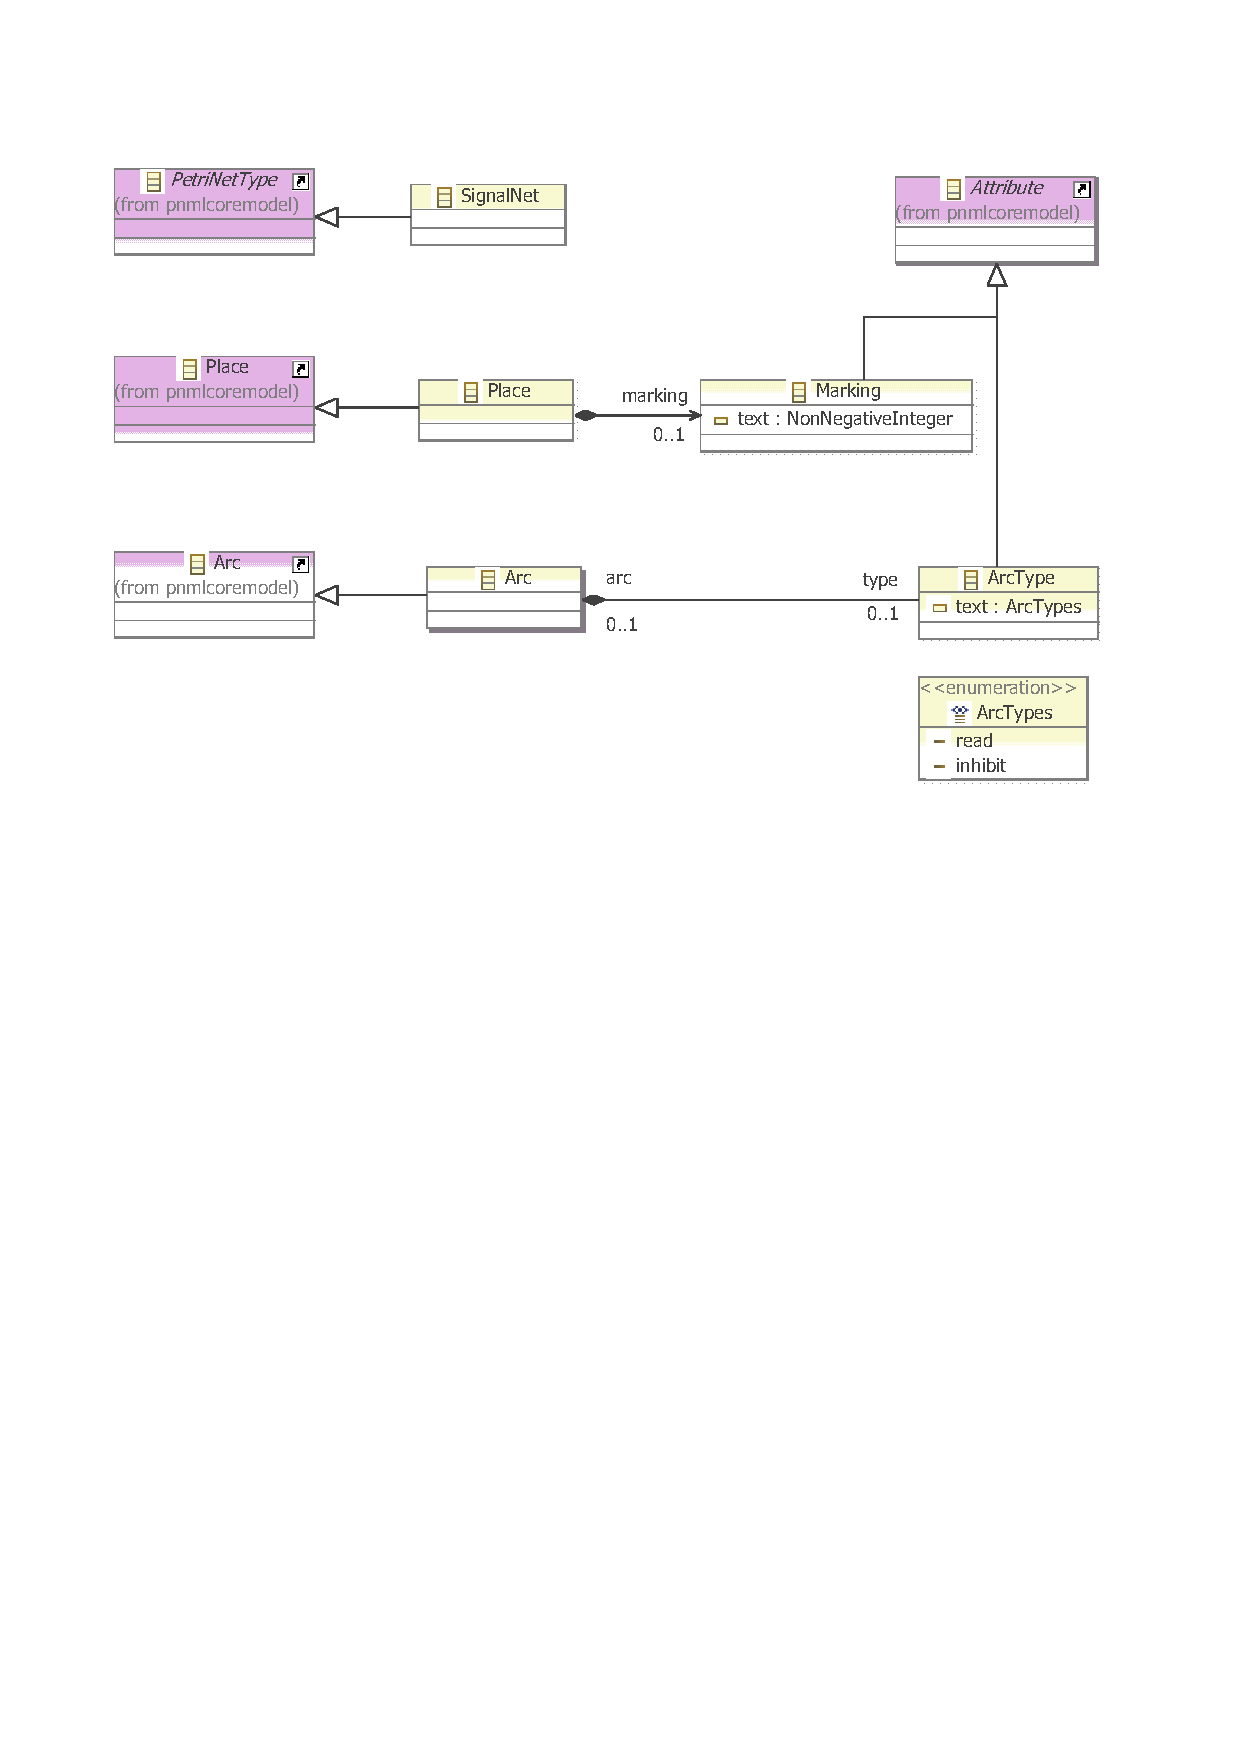
\includegraphics[scale=.60]{SE-Nets-PNTD}}
  \caption{The Ecore model for SE-Nets}
  \label{fig:SE-Nets-PNTD}
\end{figure}
%
Moreover, the Ecore model defines that there can be a {\tt Marking} for
places. Both label classes inherit from {\tt Attribute},%
  \index{ePNK!Attribute@{\tt Attribute}|DEF}
which means that these labels are not shown as annotations, but in the
properties view, when the respective arc or place are selected in the editor (see
Fig.~\ref{fig:signal-net-attributes}). We will see
Sect.~\ref{sec:dev:graphical}, how the value of these attributes can
be shown in the graphical representation
of the place or the arc. All we need to do for a label in the Petri net
type definition to be considered an attribute by the ePNK is deriving it
from the class {\tt Attribute} of the PNML core model.

If we have a closer look at the Ecore model from Fig.~\ref{fig:SE-Nets-PNTD},
we see that the class {\tt ArcType} has a reference {\tt arc} which points
back to the arc that ``owns'' that type -- the reference {\tt arc} is, actually,
an opposite of reference {\tt type}. This additional reference allows us to
navigate back from the arc type to the respective arc, which makes it easier
to formulate some constraints for arcs and their arc types\footnote
  {In the current version, this feature is not used, though.}%
. As we had discussed earlier in Sect.~\ref{subsubsec:PNTD-model}, classes
derived from {\tt Label} and also from {\tt Attribute} are not allowed to
have any feature other than the {\tt text} attribute. The reason for this
restriction is that PNML does not allow us to serialize this feature.
So, we need to make sure that such references to arcs are not serialized --
conceptually this is not necessary anyway, since the reference {\tt arc} is the opposite
of the reference {\tt type}. Therefore, we switch the serialisation
of the feature {\tt arc} off. This can done by selecting the resp.\ reference
in the editor for the Ecore model, and then, in the properties view, 
selecting the ``Advanced''\footnote
  {This ``Advanced'' section shows all kinds of advanced setting of the
   respective Ecore element. In case you are new to Ecore and you do not
   understand the concept of ``transient'', do not worry. Just ignore this for
   now.}
section, and then set the property ``transient'' to ``true'', meaning that this
feature is not serialised to a file (the ePNK serialisation mechanism takes that
into account).%
  \index{ePNK!Attribute|)}

From the Ecore model above, we can create the ``genmodel'' and generated the
model code and the edit code as discussed in Sect.~\ref{subsubsec:type-codegeneration}.
And we would need to do the same manual change: implement the {\tt toString()} method,
so that it returns the unique URI for that type; and we would need to make the
constructor of the class {\tt SignalNetImpl} public. In this example, however, we chose a
different way -- we create a class {\tt SignalNetFactory} that inherits from
{\tt SignalNetImpl} without any additional attributes, methods or constructors.
Since the implicit default constructor of {\tt SignalNetFactory} is public,
this will do the job. This is actually the preferred method, since regeneration
of the model code after a model change does not need any manual changes anymore.

Plugging in the Petri net type to the ePNK extension point works as described
in Sect.~\ref{subsubsec:simplePNTDplugin}. Listing~\ref{lst:SENetPlugin} shows
the resulting fragment of the ``plugin.xml'' (with some minor omissions).
%
\begin{figure}[htbp!]
\lstinputlisting[label=lst:SENetPlugin,language=XML,tabsize=2,stringstyle=\small,%
caption={Plugging in SE-Nets}]%
  {code/senet.xml}
\end{figure}

Listing~\ref{lst:SENetConstraint} shows the constraint for SE-nets, which makes
sure that an arc type can only be present for arcs that run from a place to a
transition; it also guarantees that arcs run from a place to a transition, from
a transition to a place, or between two transitions. It is a live constraint,
which needs to be checked, whenever the source or target of an arc are set,
and whenever the arc type is set.
%
\begin{figure}[htbp!]
\lstinputlisting[label=lst:SENetConstraint,language=XML,tabsize=2,stringstyle=\small,%
caption={Adding the constraint for SE-nets}]%
  {code/senet-constraint.xml}
\end{figure}

With these definitions, the ePNK would know what SE-nets are -- still the
inhibitor arcs and the signal arcs would not yet appear as shown in
Fig.~\ref{fig:signal-net-attributes}. To this end, we still need to
extend the graphical appearance of SE-nets, which will be discussed 
in Sect.~\ref{sec:dev:graphical}.%
  \index{SE-Nets|)}


\subsection{Petri net type definitions in general: HLPNG}
\label{subsec:complexPNTD}

In this section, we discuss some more advanced mechanisms that can be used for
defining new Petri net types. These mechanism will be discussed by the help
of the Petri net type definition of high-level Petri nets (HLPNGs). Therefore,
we start with an overview of the concepts of HLPNGs, from the implementation
point of view (for the conceptual part we refer to
Sect.~\ref{subsec:introHLPNG} and for a detailed discussion of all models and
concepts, we refer to \cite{HKea09}).

\subsubsection{Overview of HLPNGs}

As discussed in Sect.~\ref{subsec:introHLPNG}, HLPNGs have different kinds of
complex labels: \emph{declarations} of variables, sorts, and
operators; \emph{types} defining the sort of the tokens of a place,
\emph{markings} which are multiset terms defining the initial marking of a
place, \emph{conditions} as transition guards, and
\emph{arc annotations} that define which tokens are consumed, resp.\ produced
when a transition fires. What is more, the labels cannot be considered isolated from
each other anymore -- some labels, like markings, arc annotations, or
conditions may use \emph{symbols}%
  \index{ePNK!Symbol|DEF}
that are defined in other labels -- in particular, in the declarations.

Figure~\ref{fig:HLPNG-PNTD} shows the Ecore model defining the concepts of
HLPNGs, which can be found in the folder ``model'' in project\footnote
  {This is the plug-in in which HLPNGs are plugged into the ePNK; since HLPNGs
   are quite complex, and require many models, and also the implementation of
   a parser, the underlying concepts are defined in different other projects;
   all of these projects have a name with prefix {\tt
   org.pnml.tools.epnk.pntypes.hlpngs} -- some of them are generated
   automatically from models or from a grammar. You can import all
   of these projects to your workspace by the Eclipse ``Import As'' feature
   in the ``Plug-ins'' view.}
{\tt
org\qnsep{}pnml\qnsep{}tools\qnsep{}epnk\qnsep{}pntypes\qnsep{}hlpngs\qnsep{}pntd}.
This model follows the same principles as the model for PTNets, which was
discussed in Sect.~\ref{subsubsec:PNTD-model}.
%
\begin{figure} [btp!!] % [hbt!!]
  \centerline{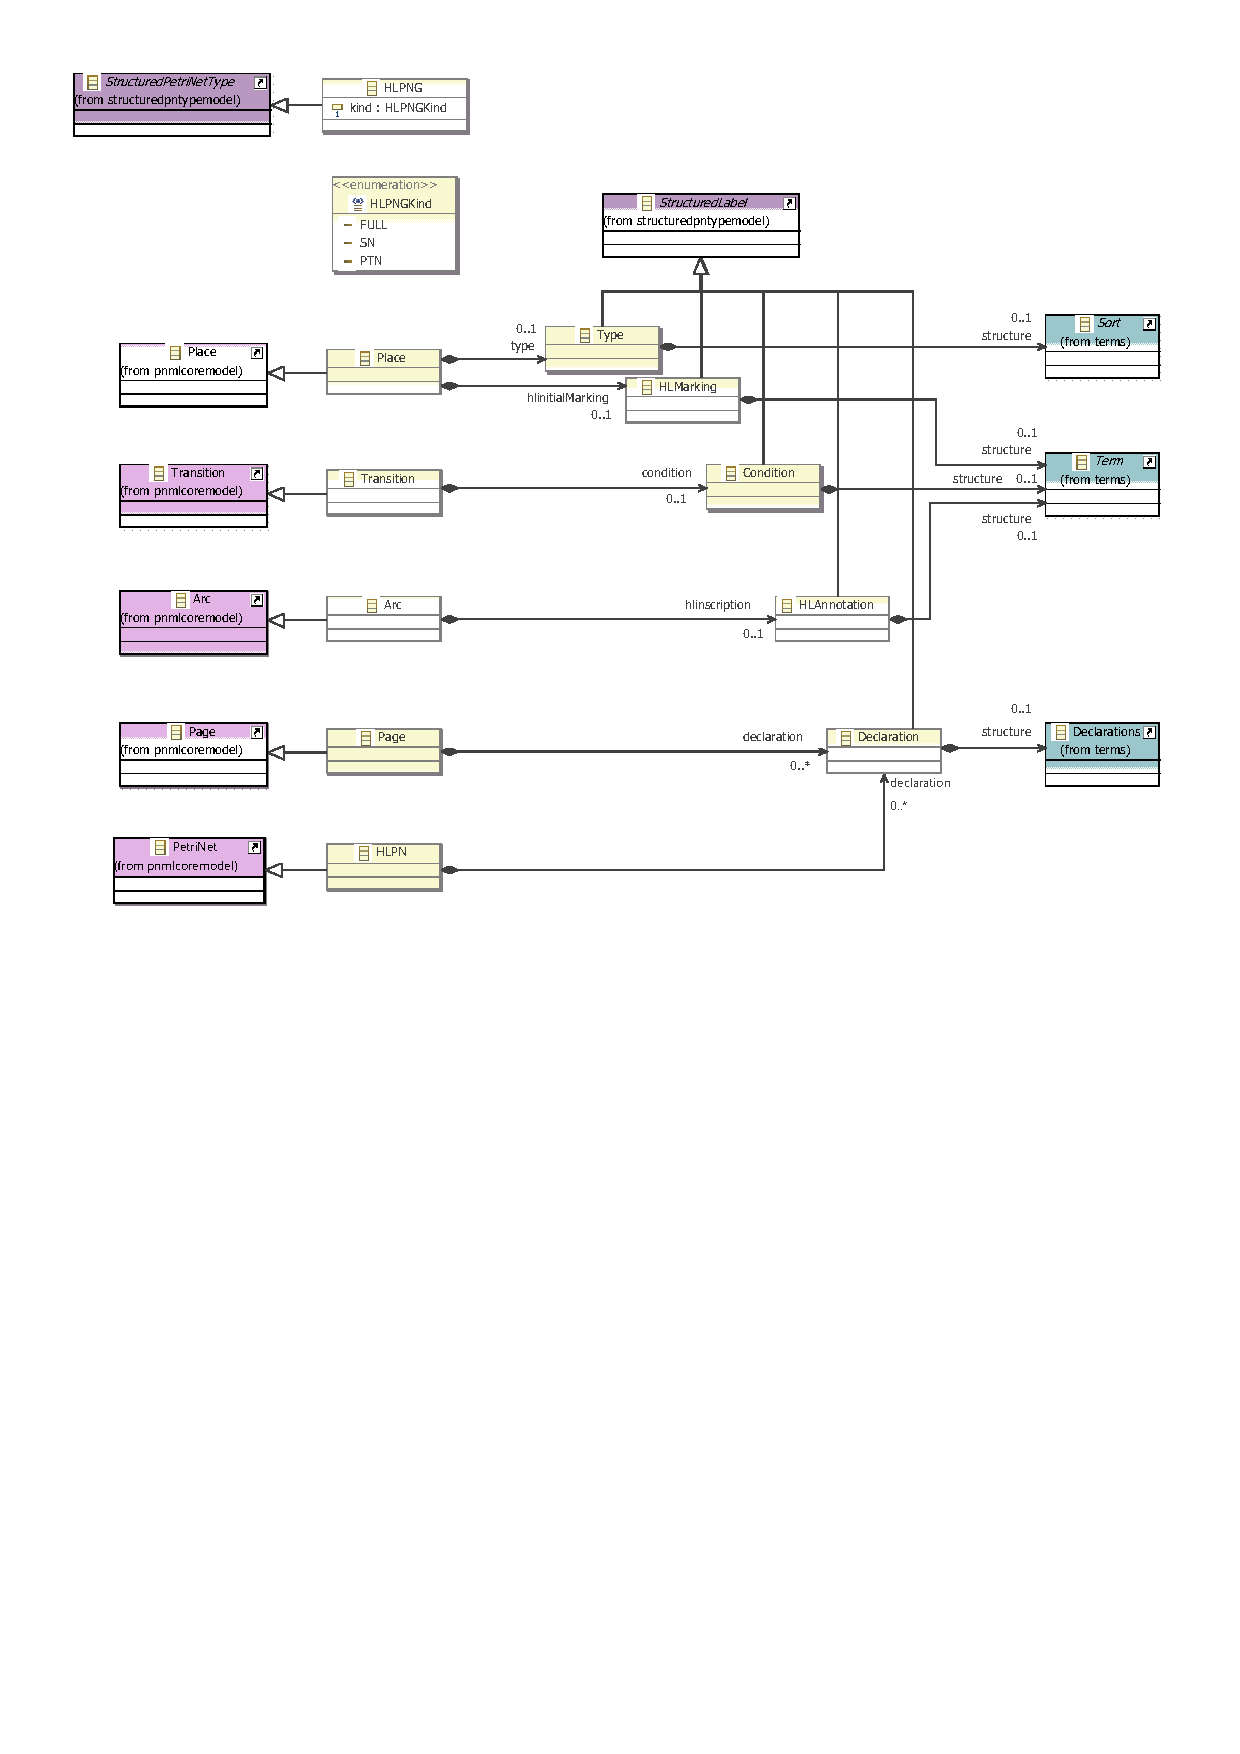
\includegraphics[scale=.67]{HLPNG}}
  \caption{The Ecore model for HLPNGs}
  \label{fig:HLPNG-PNTD}
\end{figure}
%
The main differences are that the defined Petri net type {\tt HLPNG} extends a
more advanced class {\tt StructuredPetriNetType}, and all labels extend
{\tt StructuredLabel}, which are part of the PNML core model. These two classes
provide the infrastructure needed for parsing the textual labels and for
establishing the links between these labels. This structure is discussed
in Sect.~\ref{subsubsec:structuredPNTs}.  

The actual contents of all these labels is defined in their containment {\tt
structure}; note that we use {\tt Term} as the contents for the labels {\tt
HLMarking}, {\tt Condition}, and {\tt HLAnnotation}, since all of them are terms -- just
with different additional constraints imposed on them (see
Sect.~\ref{subsubsec:PNTDConstraints}).
Note that by contrast to normal labels and attributes, \emph{structured labels}
can have -- actually must have -- a composition, which normally\footnote
  {The name could be changed, but this would require some programming, which
   will be discussed later.}
has the name {\tt structure}. But there should not be any other features than
that.

The detailed structure and concepts of terms, sorts, and declarations, are
defined in several other models. Since these details are not too relevant
for understanding the definition of structured Petri net types, we discuss
only the main part of that model.
%
\begin{figure}[btp!!] % [hbt!!]
  \centerline{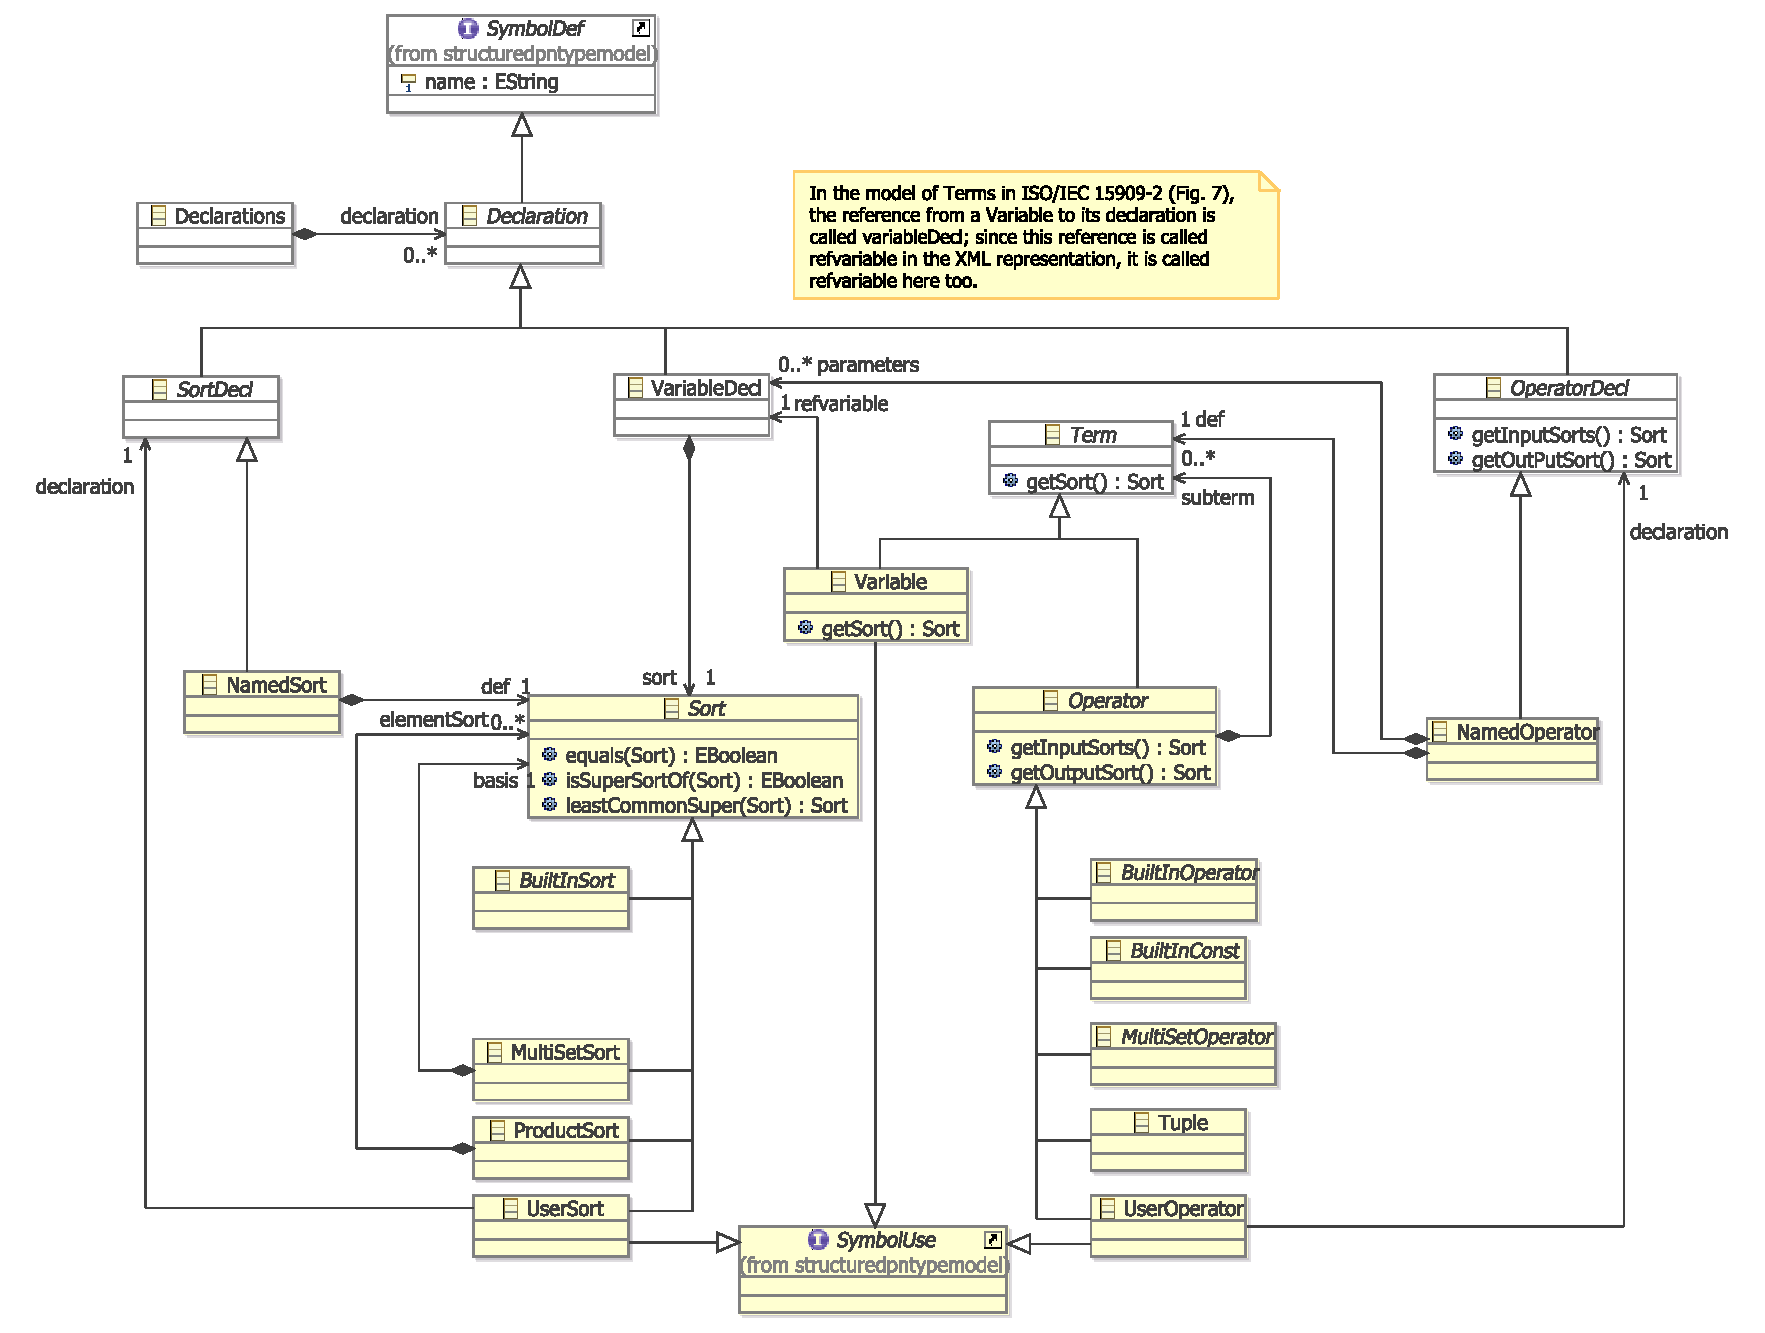
\includegraphics[scale=.45]{HLPNGDataTypes-Terms}}
  \caption{The Ecore model for the main concepts of HLPNGs}
  \label{fig:HLPNG-Terms}
\end{figure}
%
This part of the model is shown in Fig.~\ref{fig:HLPNG-Terms} -- this as well as
the diagrams of all the other models can be found in the plug-in {\tt
org.pnml.tools.epnk.pntypes.hlpngs.datatypes}. For a detailed discussion of
these models and their concepts, we refer to \cite{HKea09}. There is only one
important difference, which are the classes {\tt SymbolDef}%
  \index{ePNK!SymbolDef@{\tt SymbolDef}|DEF}
and {\tt SymbolUse},%
  \index{ePNK!SymbolUse@{\tt SymbolUse}|DEF}
which do not occur in the models of ISO/IEC~15909-2. 
These two classes are the ePNKs infrastructure for dealing with the definition
of symbols and their use in a uniform and generic way -- on the side, making the
concepts of \emph{symbol definition}%
  \index{ePNK!Symbol definition|DEF}
and \emph{symbol use}%
  \index{ePNK!Symbol use|DEF}
explicit, so that the model is more concise. These concepts are part of
the PNML core model concerning structured Petri net types, which will be
discussed in the next section.

\index{Net label|(DEF}%
One other issue worth noting in the Ecore model of Fig.~\ref{fig:HLPNG-PNTD} is
the class {\tt HLPN}, which extends class {\tt PetriNet}%
  \index{ePNK!PetriNet@{\tt PetriNet}|DEF}
from the PNML core model. This represents the Petri net itself. Normally, Ecore
models defining a new Petri net type would not need to extend the class
{\tt PetriNet} itself; it would be enough to extend the class {\tt
PetriNetType}.%
  \index{ePNK!PetriNetType@{\tt PetriNetType}|DEF}
HLPNGs, however, have so-called \emph{net labels},
which are labels that are directly attached
to the net -- and not to a page. For net types with net labels, the class
{\tt PetriNet} must be extended and equipped with compositions to the respective
labels -- in our example, these are declarations. But, we would
discourage defining such net labels for Petri nets types.%
\index{Net label|)}

\subsubsection{Structured Petri net types and structured labels}
\label{subsubsec:structuredPNTs}
\index{ePNK!structured Petri net type|(DEF}
\index{ePNK!structured label|(DEF}

As mentioned above, the ePNK provides some general interfaces and infrastructure
for defining structured Petri net types, which distill the general concepts of
more complex Petri net types. This is, again, captured in models (and the
code generated from them).

The model for structured Petri net types can be found in the ``model''
folder of the ePNK core project {\tt org\qnsep{}pnml\qnsep{}tools\qnsep{}epnk}:
{\tt PNMLStructured\optsep{}PNTypeModel}.
The diagram is shown in Fig.~\ref{fig:PNMLStructuredType}.
%
\begin{figure}[hbt!!]
  \centerline{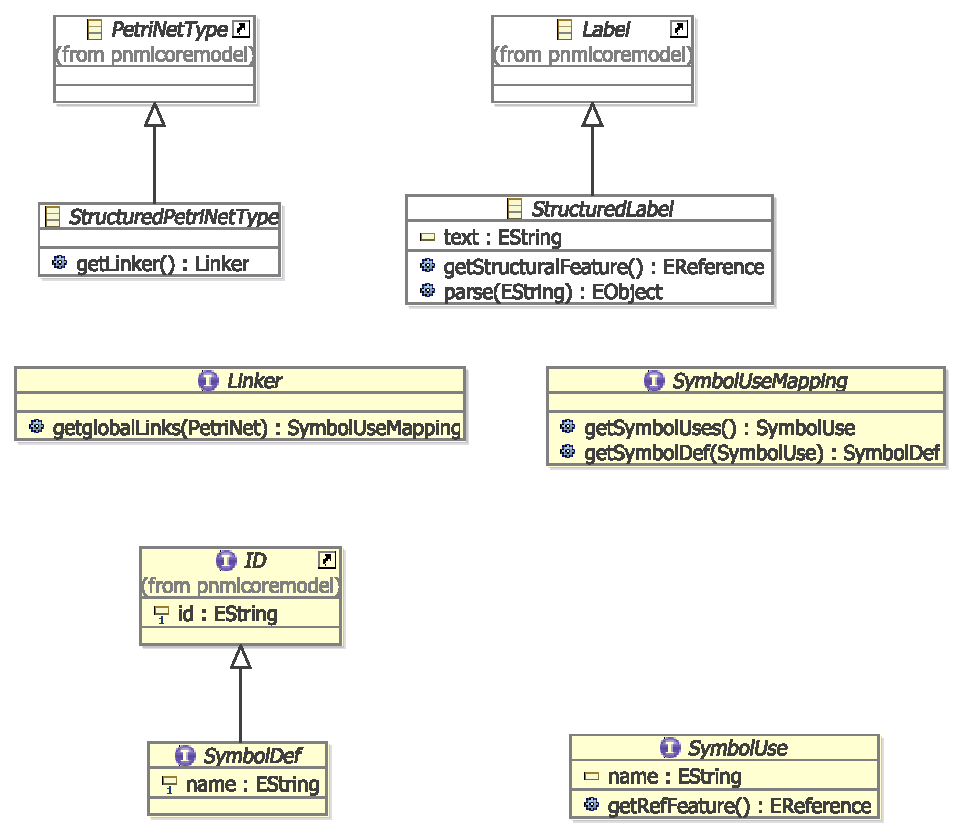
\includegraphics[scale=.60]{PNMLStructuredPNTypeModel}}
  \caption{The model for structured Petri net types}
  \label{fig:PNMLStructuredType}
\end{figure}
%
We know the classes {\tt PetriNetType} and {\tt Label} as well as the
interface {\tt ID}, which is used for all ePNK elements that have an id,
already from the PNML core model. The abstract class {\tt StructuredLabel}%
  \index{ePNK!StructuredLabel@{\tt StructuredLabel}|DEF}
extends the class {\tt Label}, it has an attribute {\tt text}, which stores
the contents of this label as a text String. The actual structural contents
is defined by classes that extend it (we have seen
some examples in Fig.~\ref{fig:HLPNG-PNTD} already). Since, the ePNK cannot
not know these concrete implementations, classes extending the structural
label must make the reference to this structural contents known to the
ePNK. This is achieved by the method {\tt getStructuralFeature()};%
  \index{ePNK!getStructuralFeature@{\tt getStructuralFeature()}|DEF}
as long as the feature for the structure is called `structure' in the model, we
do not need to do anything in the implementation (the ePNK will access this
feature in a reflective way); only if for some reason, the model chooses a
different name, this method must be implemented manually. Moreover, every class
for a structural label must provide a method {\tt parse()}%
  \index{ePNK!parse@{\tt parse()}|DEF}
for parsing a String
-- a representation of this label in concrete syntax; an implementation of this
method may return null, if the text cannot be parsed. If the label could be
parsed,  it must return some object (to be precise an {\tt EObject} which is the
EMF version of objects) with all the substructure of that label -- the abstract
syntax of the label. In particular, that object must have a type that is
compatible with the label's structural feature. This method must be implemented
manually for every new extension since the ePNK cannot guess the concrete syntax.

The abstract class {\tt StructuredPetriNetType}%
  \index{ePNK!StructuredPetriNetType@{\tt StructuredPetriNetType}|DEF}
has one additional method, which must provide a {\tt Linker}%
  \index{ePNK!Linker@{\tt Linker}|DEF} 
for linking the uses of some symbols to their definitions, which are captured by
classes {\tt SymbolDef}%
  \index{ePNK!SymbolDef@{\tt SymbolDef}|DEF}
and {\tt SymbolUse}.%
  \index{ePNK!SymbolDUse@{\tt SymbolUse}|DEF} 
A {\tt SymbolDef} has an {\tt ID}%
  \index{ePNK!ID@{\tt ID}|DEF} 
and has a name, which will be used to refer to it (the id is internal to PNML
and the ePNK). This name will be used in {\tt SymbolUse}, again as
attribute name, to refer to the definition. The feature that actually refers to the definition, can
be accessed via the method {\tt getRefFeature()}.%
  \index{ePNK!getRefFeature@{\tt getRefFeature()}|DEF}
Since the ePNK does not know anything about how to make these connections, the
Petri net type needs to provide access to the linker; to this end, the class
{\tt StructuredPetriNetType} has a method {\tt getLinker()},%
  \index{ePNK!getLinker@{\tt getLinker()}|DEF}
which must be implemented by classes that extend it. {\tt Linker} is an
interface: a single method {\tt getglobalLinks()},%
  \index{ePNK!getglobalLinks@{\tt getglobalLinks()}|DEF}
which takes a Petri net and returns a {\tt SymbolUseMapping},%
  \index{ePNK!SymbolUseMapping@{\tt SymbolUseMapping}|DEF}
which is also an interface. Conceptually, the class {\tt SymbolUseMapping} maps
every {\tt SymbolUse} to its definition {\tt SymbolDef}. All the symbol uses for
which there exists a mapping, can be obtained (as a list) via the method
{\tt getSymbolUses()};%
  \index{ePNK!getSymbolUses@{\tt getSymbolUses()}|DEF}
and for each symbol use, the method
{\tt getSymbolDef()}%
  \index{ePNK!getSymbolDef@{\tt getSymbolDef()}|DEF}
will return the definition of that symbol. 

With this infrastructure, the ePNK can deal with all kinds of structured
labels. We will have a look at the implementation of some examples next:  We
consider the label {\tt Condition} in the Petri net type definition for HLPNGs
again (see Fig.~\ref{fig:HLPNG-PNTD}) -- the other labels are similar. Its
structural feature is the containment {\tt structure} to class {\tt Term}.
Since this is the standard name for structured labels, we do not need to
override the method {\tt getStructuralFeature}.%
  \index{ePNK!getStructuralFeature@{\tt getStructuralFeature}|DEF}
But, we need to implement the {\tt parse()} method.  The parsers for all labels
of HLPNGs were automatically generated by Xtext, and are made available in a
singleton class {\tt HLPNGParser} in package
{\tt org.pnml.tools.epnk.pntypes.hlpngs.datatypes.concretesyntax}
in a project with the same name. For parsing a term, class {\tt HLPNGParser}
provides a method {\tt parseTerm(String)}. This singleton and its method
{\tt parseTerm()} is used in the implementation of {\tt ConditionImpl}
(you will find it in the package
{\tt org.pnml.tools.epnk.pntypes.hlpng.pntd.hlpngdefinition.impl}
in project {\tt org.pnml.tools.epnk.pntypes.hlpng.pntd}).

Since linking is across all the different labels of a net, there is only a
single linker for every net. For HLPNGs, this is implemented in the package
{\tt org\qnsep{}pnml\qnsep{}tools\qnsep{}epnk\qnsep{}pntypes\qnsep{}hlpngs\qnsep{}datatypes\qnsep{}concretesyntax\qnsep{}linking}
in project {\tt
org\qnsep{}pnml\qnsep{}tools\qnsep{}epnk\qnsep{}pntypes\qnsep{}hlpngs\qnsep{}datatypes\qnsep{}concretesyntax}.
This class is {\tt HLPNGLinker}; basically it goes through the complete Petri net twice; in the first round, it creates a symbol table of all symbol
definitions; in the second round, this symbol table is used to look up the
definition for every symbol use, which is stored in the {\tt SymbolMapping},
which implements the {\tt SymbolUseMapping} that we discussed above.

To make this linker known to the ePNK, the class {\tt HLPNGImpl} in
package {\tt
org.pnml.tools.epnk.pntypes.hlpng.pntd.hlpngdefinition.impl} implements the
method {\tt getLinker()}: it returns an instance of {\tt HLPNGLinker}.

Note that, in order to plug in the Petri net type definition to the ePNK,
we need to make the constructor public in the
class {\tt HLPNGImpl}, and we need to implement the {\tt toString()} method
so that it returns the unique URI of HLPNGs method
(as discussed in Sect.~\ref{subsubsec:simplePNTDplugin}).%
  \index{ePNK!structured Petri net type|)}%
  \index{ePNK!structured label|)}

\subsubsection{Constraints}
\label{subsubsec:PNTDConstraints}
\index{ePNK!Constraints|(DEF}
\index{ePNK!Java constraint|(DEF}

For HLPNGs, we needed to implement quite many constraints. As an example
for a \emph{Java constraint}, we discuss one of these constraints here. The rest
of them would not provide much insight into the mechanisms of the ePNK -- though they
might provide some insights to the inner workings of HLPNGs themselves.
There is also an OCL constraint that forbids connecting places with places
and transitions with transitions. But, this is exactly the same as for PTNets,
which is why we do not discuss it here again.

All constraints for HLPNGs are defined in the project
{\tt
org\qnsep{}pnml\qnsep{}tools\qnsep{}epnk\qnsep{}pntypes\qnsep{}hlpng\qnsep{}pntd},
the implementations of the Java constraints can be found in the package
{\tt org\qnsep{}pnml\qnsep{}tools\qnsep{}epnk\qnsep{}pntypes\qnsep{}hlpng\qnsep{}pntd\qnsep{}validation}
We discuss the constraint that transition conditions must have type boolean,
which is implemented in class {\tt ConditionIsBoolType}.
Listing~\ref{lst:constraintCondIsBool} shows this class.
%
\begin{figure}[htbp!]
\lstinputlisting[label=lst:constraintCondIsBool,tabsize=2,stringstyle=\small,%
caption={The constraint that conditions have type boolean}]%
{code/ConditionIsBoolType.java}
\end{figure}
%
This constraint extends the class {\tt AbstractModel\optsep{}Constraint}%
  \index{EMF!AbstractModelConstraint@{\tt AbstractModelConstraint}|DEF}
from EMF Validation and implements the method {\tt validate()}.%
  \index{EMF!validate@{\tt validate()}|DEF}
From the validation context, it obtains the target object, which should be a
transition (see later). But, we are defensive and check that explicitly. Then, we
obtain the condition label of that transition, and if it is not {\tt null},
get the term (its structure). Then, we check whether the sort of
the term is boolean\footnote
 {The implementation of {\tt getSort()} for terms is actually quite
  complex; it amounts to implementing a type system for the
  annotation language of HLPNGs. But we do not discuss the details here.}%
. If it is not, we return a failure status via the validation context,
and add the transition and the textual label to an array of objects
(which is used in the error message to be defined later). Otherwise,
we return a success status. Note that the EMF Validation Framework
makes sure that this validate method is called for all transitions
of a selected Petri net, Petri net document or page, once it is
properly plugged in, which is discuss below.

Plugging in a Java constraint is similar to plugging in
OCL constraints. The relevant fragment of the ``plugin.xml''
is shown in Listing~\ref{lst:HLPNGJavaConstraint}.
%
\begin{figure}[htbp!]
\lstinputlisting[label=lst:HLPNGJavaConstraint,language=XML,tabsize=2,stringstyle=\small,%
caption={Adding the constraint for conditions}]%
  {code/hlpng-constraint.xml}
\end{figure}
%
The main differences are that the attribute {\tt lang} is ``Java''
now and the attribute {\tt class} refers to the class {\tt ConditionIsBoolType},
which was discussed above. As target class, the transition class of
HLPNGs is defined (that is why we could assume that the target
object is a transition). Another difference is that this is no live constraint,
but a batch constrain. This means, that the constraint might be violated during
editing; a violation will be detected and reported only when the user
explicitly invokes the validation.
Since this is a batch constraint, we do not need to declare any events in
the target.

Another difference to the OCL constraint is, that we can refer to several
parameters in the message now. What the different parameters are, depends
on the return value of the validation method. In our case, this was
the transition (or its String representation) and the text of the label.

The ellipses (``...'') indicate that the constraint that we have discussed
here, is just one of many other constraint, which are not discussed here.%
  \index{ePNK!Constraints|)}
  \index{ePNK!Java constraint|)}

\subsubsection{XML Mappings}
\label{subsubsec:XMLmapping}
\index{ePNK!XML mapping|(DEF}

In the sections above, we have discussed how to define a Petri net type and
all its concepts and constraints. For saving it in PNML, it is also necessary
to define how these concepts are represented in XML -- at least if the
``standard mappings'' do not work.

In this section, we discuss how these mappings are defined. Conceptually,
these mappings are tables (in ISO/IEC~15909-2, these tables are given
in Clause~7.3.1). In the ePNK, these tables are ``programmed'' as part
of the new Petri net type\footnote
  {It might be, that a future version of the ePNK will provide a means to plug
  in these tables directly in some form; but since ``programming the tables'' is
   not too difficult, this does not have a high priority.}%
.  

We explain the concepts of these ``programmed tables'' by discussing some
of the mappings for HLPNGs. The tables for a new Petri net type are
programmed, by overwriting the method
{\tt registerExtended\optsep{}PNMLMetaData(\optsep{}ExtendedPNMLMetaData
metadata)} of {\tt PetriNetType}; the parameter {\tt meta\optsep{}data}
represents the table, to which the entries should be added when the method is called.

Let us have a look at some examples. Listing~\ref{lst:xml-simple-mapping} shows
an excerpt of the {\tt registerExtendedPNMLMetaData()}%
  \index{ePNK!registerExtendedPNMLMetaData@{\tt
  registerExtended PNMLMetaData()}|DEF} method of the class {\tt HLPNGImpl},
  which implements the Petri net type for HLPNGs.
%
\begin{figure}[htbp!]
\lstinputlisting[label=lst:xml-simple-mapping,tabsize=2,stringstyle=\small,%
caption={Mappings for type, marking, and condition extensions}]%
{code/xml-mapping-simple.java}
\end{figure}
%
Each of the {\tt metadata.add} statements defines one table entry, which
defines the mapping of one specific feature of the Ecore model to an
XML element (we will see later how to map an Ecore attribute to an XML
attribute). The three statements shown in Listing~\ref{lst:xml-simple-mapping}
define how the structure feature of the labels {\tt Type}, the {\tt HLMarking},
and the {\tt Condition} are mapped to the XML element {\tt \verb+<structure>+}.
We discuss the first one, the {\tt Type}, in more detail:
\begin{itemize}
  \item The first parameter, denotes the feature that is mapped to XML by this
        entry; in this case, it is the composition from the class {\tt Type} to
        the class {\tt Sort} (see Fig.~\ref{fig:HLPNG-PNTD} on
        page~\pageref{fig:HLPNG-PNTD}). The source and target classes are
        mentioned explicitly as second and third parameter again. We refer to
        the feature and the two classes via the singleton classes that describes
        the elements of the packages (HLPNGdefinition and Terms), which
        are automatically generated by EMF. These
        \emph{package classes},%
			\index{EMF!Package class}
        provide access to all the classes and features
        within a package (see \cite{BSM06} for more details). Note that {\tt
        HlpngdefinitionPackage.eINSTANCE} refers to the package {\tt
        hlpngdefinition} and {\tt TermsPackage.eINSTANCE} to the package {\tt
        terms}.
        
  \item As mentioned above, the second parameter denotes the class to
        which the feature belongs (it could be a sub-class of {\tt Type}
        in principle); this is often called the \emph{container class}.%
          \index{EMF!Container class|DEF}
        
  \item The third parameter denotes the class that the feature refers to
        (this could also be a sub class of {\tt Sort}); this is often called the
        \emph{object class}.%
          \index{EMF!Object class|DEF}
        
  \item The forth parameter defines the XML representation, the string
        that will be used as XML element in the serialisation of this
        feature (in our example ``structure'').
        
  \item The fifth parameter could refer to an XML attribute, that might
        be necessary for creating an Ecore object from the XML element
        (we will discuss an example later). In most cases, this XML attribute
        is not needed, since the XML element (and the context in which it
        occurs) provide enough information for creating the Ecore element from
        it.
        
  \item The last parameter refers to a factory that is capable of creating
        an Ecore instance of the respective class from the XML element
        and -- if provided -- the XML attribute. This parameter can
        be left empty, when the Ecore instance can be constructed reflectively
        from the information on the object class only.   
\end{itemize}

The ePNK uses this table and its entries in two directions: In the one
direction, the table is used to serialise a Petri net to its XML
syntax; in the other direction, the table is used to create the model
elements from the XML syntax.
In the latter case, the \emph{factories}%
  \index{ePNK!Factory|DEF}%
  \index{ePNK!IPNMLFactory@{\tt IPNMLFactory}|DEF}
play an important role. Listing~\ref{lst:factory-interface} shows the interface
that all these factories must implement.
%
\begin{figure}[htbp!]
\lstinputlisting[label=lst:factory-interface,tabsize=2,stringstyle=\small,%
caption={Interface {\tt Factory}}]%
{code/IPNMLFactory.java}
\end{figure}
%
The methods {\tt canCreateObject()}%
  \index{ePNK!canCreateObject@{\tt canCreateObject()}|DEF}
and {\tt createObject()}%
  \index{ePNK!createObject@{\tt createObject()}|DEF}
have the same parameters, which basically reflect the entries of the table that
we discussed above. Only the third (representing the object class) and the six one
(the factory itself) are missing. And, there is an additional parameter
({\tt provider}), which will provide access to the values of all attributes of
the currently read XML element (in case the factory needs the values of some
of the XML element's attributes for creating an object of the appropriate type).
The method {\tt canCreateObject()} is used to find out whether the factory is able
to create an object from the provided information, the {\tt createObject()}
method is used to actually create it. The {\tt createAttributeObject} is
used to create an object for some XML attribute. The implementation of these
factories is straightforward and a bit boring -- we do not discuss the
details here. You can have a look into the class {\tt HLPNGFactory}
in package {\tt
org\qnsep{}pnml\qnsep{}tools\qnsep{}epnk\qnsep{}pntypes\qnsep{}hlpng\qnsep{}pntd\qnsep{}hlpngserialisation\qnsep{}factory}
in the project {\tt org\qnsep{}pnml\qnsep{}tools\qnsep{}epnk\qnsep{}pntypes\qnsep{}hlpng\qnsep{}pntd} to get some
inspiration. What is more, with an extension that came into version 0.9.0
of the ePNK, the factory can be set to {\tt null}. In which case the
standard mechanism for creating an object of the target class will
be used; therefore, we need factories only in very special
cases. In most of the cases, the factory can be set to {\tt null}\footnote
  {Note that except for two features, which were used to test this
   new mechanism, the mappings for HLPNGs have not been updated 
   yet; therefore, you will find factories all over these mappings.
   But, this has historic reasons only and will eventually be
   changed (making the mappings more maintainable and easier to understand).}%
.

\begin{figure}[tbp!] % [htbp!]
\lstinputlisting[label=lst:xml-attribute-mapping,tabsize=2,stringstyle=\small,%
caption={Mappings of an attribute}]%
{code/xml-attribute-mapping.java}
\end{figure}
%
Listing~\ref{lst:xml-attribute-mapping} shows an example\footnote
  {Actually, this is the only example of this kind in HLPNGs.}
of how a feature of the model can be mapped to an XML attribute. In this
example, the value of the boolean constant is mapped to the XML attribute 
{\tt value}. This is where the method {\tt createAttributeObject()}%
  \index{ePNK!createAttributeObject@{\tt createAttributeObject()}|DEF}
of the factory comes into play.

The discussion above, gives a general idea of how these tables and mappings
work. All this, however, could have been achieved with the existing mechanisms
of EMF: Extended Metadata. Some of the PNML constructs cannot be
mapped to XML by the mechanisms provided by EMF Extended Metadata.
Therefore, the ePNK needed to provide its own mechanism for mapping
Ecore concepts to XML. In the rest of this section, we discuss some of
these special situations.

To this end, we consider the serialisation of the simple term {\tt
x`f(x,x)}, where {\tt x} is a variable and {\tt f} is a user defined operator.
The PNML representation is shown in Listing~\ref{lst:subterm-xml}, where ``5''
is the unique id of variable {\tt x} and ``1'' is the id of the user defined
operator {\tt f},
%
\begin{figure}[tbp!] % [htbp!]
\lstinputlisting[label=lst:subterm-xml,language=XML,tabsize=2,stringstyle=\small,%
caption={PNML representation of {\tt x`f(x,x)}}]%
{code/subterm.xml}
\end{figure}
%
In addition to being a bit verbose, there is one thing that is special about
this mapping: There is an XML element \verb+<subterm>+ for the association
form the top-level term (number of) to its subterm,
which are represented as two other XML elements,
\verb+<variable>+  and \verb+<useroperator>+. The XML element 
\verb+<subterm>+ defines to which feature of the term the XML element that is
contained in it should go. The XML element inside (e.\,g.\ 
\verb+<variable>+) defines the type that this object should have.

The problem here, is that there is an intermediate XML element that has no
object as counter part in the model -- it represents an association. We call
such an XML element an \emph{association element}.%
  \index{ePNK!Association element|DEF}
The mapping for these association elements is shown in
Listing~\ref{lst:xml-assoc-mapping}.
%
\begin{figure}[htbp!]
\lstinputlisting[label=lst:xml-assoc-mapping,tabsize=2,stringstyle=\small,%
caption={Mappings of associations to XML elements}]%
{code/xml-assoc-mapping.java}
\end{figure}
%
The first entry is actually as we have seen it before. The only difference
is that the factory produces an instance of a new class
{\tt TermAssoc}, which has the nature of a term but, actually, represents
an association to a term. We will discuss that class in more
detail later. The two other mappings, define the mapping of variables
and user operators to XML, and these are different, since they do not
refer to any feature at all. They just refer to a container class and 
a contained class. The container class is the class {\tt TermAssoc},
which will make sure that the variable resp.\ user operator will be added
to the subterm feature of the operator on the level above\footnote
  {There would actually be another way of doing this, in a slightly more
   elegant way when using ``standard features'', which
   will be discussed later in this section.}%
.

The class {\tt TermAssoc} does not need to be programmed. This class,
as well as the other classes for representing association elements, could
completely be generated from a model. This model is shown in Fig.~\ref{fig:AssocClasses}.
These classes extend a specific class of our model (the one to which the
respective association should go), and the general class for {\tt AssocClass},
which is defined by the ePNK, and implements all the necessary functionality.
%
\begin{figure}[btp!!]% [hbt!!]
  \centerline{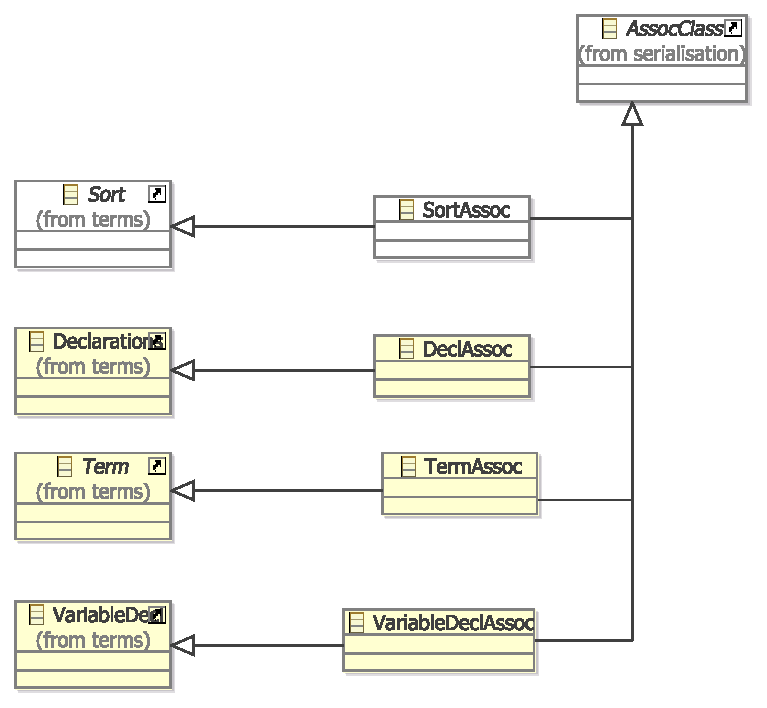
\includegraphics[scale=.60]{HLPNGSerialisation}}
  \caption{The package {\tt hlpngserialisation}}
  \label{fig:AssocClasses}
\end{figure}
%
Note that these classes will not occur in the model anymore, once it is
completely loaded -- they are only used while a PNML file is loaded.

In the case of subterms, every subterm occurs in a separate \verb+<subterm>+
element -- even if a term has several subterms, there is one subterm element
for each of them (see Listing~\ref{lst:subterm-xml}). In the case of parameters
of an operation declaration, this is different: Listing~\ref{lst:xml-parameters}
shows the PNML representation of the declaration of a named operator
{\tt f(x:INT, y:INT) =  x * y}.
%
\begin{figure}[htbp!]
\lstinputlisting[label=lst:xml-parameters,language=XML,tabsize=2,stringstyle=\small,%
caption={PNML structure for declaration {\tt f(x:INT, y:INT) =  x * y}}]%
{code/parameters.xml}
\end{figure}
%
Here, all variable declarations occur in the same \verb+<parameter>+ element.
We called these \emph{bundled association elements}.%
  \index{ePNK!bundled association element|DEF}
The table entries for this
mapping are shown in Listing~\ref{lst:xml-bundles}. The first one, is almost the
same as for association elements, and the Factory {\tt HLPNGFactory}
would create an instance of {\tt VariableDeclAssoc} for an XML element
\verb+<parameter>+. The new last parameter {\tt true} says, that this is
a bundled association.
%
\begin{figure}[tbp!]
\lstinputlisting[label=lst:xml-bundles,tabsize=2,stringstyle=\small,%
caption={Mapping bundled association elements}]%
{code/xml-bundles.java}
\end{figure}
%
The second table entry defines the mappings for variable entries, which
is independent of the context, which is why the first to parameters are
{\tt null}. We call this a \emph{context independent element mapping}.%
  \index{ePNK!context independent element|DEF}
  
This context independent element mapping can be applied in any other
context. In combination with another special case of mappings which we
call \emph{standard feature},%
  \index{ePNK!standard feature|DEF}
this is a very powerful mechanism. For example, for {\tt Declarations} and
sub-elements for which context independent element mappings exist (in the
example, there would be variable declarations, sort declarations, and
operator declarations), all these elements should be added to this standard
feature. The table entry shown in Listing~\ref{lst:xml-standard-feature} defines
the composition {\tt declaration} as the standard feature of {\tt Declarations}.
%
\begin{figure}[htbp!]
\lstinputlisting[label=lst:xml-standard-feature,tabsize=2,stringstyle=\small,%
caption={Defining a standard feature}]%
{code/xml-standard-feature.java}
\end{figure}
%
Note that there is no mapping to XML here. A standard feature of an element just
says that, whenever there comes some context independent element that is not
mapped explicitly to a feature, this element should be added to the standard
feature of the model. Of course, there should only be one standard feature --
otherwise there would be some ambiguities.%
  \index{ePNK!XML mapping|)}

\subsection{Petri net type definitions: Summary and overview}
\label{subsec:pntd:summary}

In Sect.~\ref{subsec:simplePNTD}--\ref{subsec:complexPNTD}, we have seen most
of the mechanisms for defining new Petri net types. Basically, a Petri net
type definition  consists of a new Ecore package where the Petri net
type of the PNML core model is extended and the classes for the extended Petri
net elements are modelled. Form this model the major parts of the code
(model and edit code) can be generated. In the generated code, some
manual changes need to be made. The Ecore package needs to follow some
modelling principles that are discussed in Sect.~\ref{subsubsec:PNTD-model} and
the manual changes are discussed in Sect.~\ref{subsubsec:type-codegeneration}.
All the extensions must be added as \emph{labels} of the respective kind
of node of the Petri net.

If a label should not be shown as annotation of the respective element
in the graphical editor of the ePNK, this can be achieved by deriving it from
the ePNK class {\tt Attribute}. Attributes can be edited in the properties view
of the ePNK only. Sect.~\ref{subsec:PNTD:SE-Nets} discussed an example.

More complex Petri net types might require to also implement a parser
and to store the actual information of the label not only as text but also
as an abstract syntax tree in the PNML file. Such labels are called
structured labels and have been discussed in
Sect.~\ref{subsubsec:structuredPNTs}. In case of complex Petri net types,
it might also be necessary to customize the XML representation, of the
labels and the concepts of its abstract syntax. To this end, the ePNK
allows Petri net types to define a XML mapping, which is discussed in
Sect.~\ref{subsubsec:XMLmapping}.

For all kinds of nets, it is possible to add additional constraints
on top of the Ecore model of the respective type. These constraints are
plugged in via the standard mechanisms for EMF Validation. Two examples
are discussed in Sect.~\ref{subsubsec:simplePNTDconstraints} and
Sect.~\ref{subsubsec:PNTDConstraints}. The constrains can either be
programmed in Java or can be OCL.

Note that it is possible to extend the class {\tt PetriNet} of
the PNML core model (when net labels are needed in the Petri net type).
It is also possible to add labels to pages and reference nodes by
extending the respective classes in the Ecore model for the new
Petri net type.

When an annotation is defined for a page, the question is whether the
respective annotation should be shown as a label annotated to the
node page on the super page or whether the label should be shown
as a page label on the page itself. The name of a page is
  \index{ePNK!Page label|DEF}
shown as an annotation of the page on the super page; by default, an
annotation of a page is shown as page labels on the page itself,
if there can be multiple annotations of that kind for the page;
and it is shown as a label of the page node on the super page,
if there can be only one annotation of that kind. But, this can
be changed by overriding the method {\tt showLabelOnPage()}%
  \index{ePNK!showLabelOnPage@{\tt showLabelOnPage()}|DEF}
of the class {\tt Page} of the respective Petri net type -- which requires
manual coding again.%
  \index{ePNK!Petri net type definition|)} 


\section{Defining the graphical appearance}
\label{sec:dev:graphical}

For some kinds or Petri nets, some places, transitions or arcs should be
shown in a dedicated graphical representation. And the graphical appearance
might depend on the context of the respective element -- and the graphical
appearance might change dependent on the changes of the context of this element.
An example are signal arcs, inhibitor arcs, and read arcs in SE-nets, an
example of which is shown in Fig.~\ref{fig:dev:signal-net-graphics} again.

\begin{figure}[hbt!!]
  \centerline{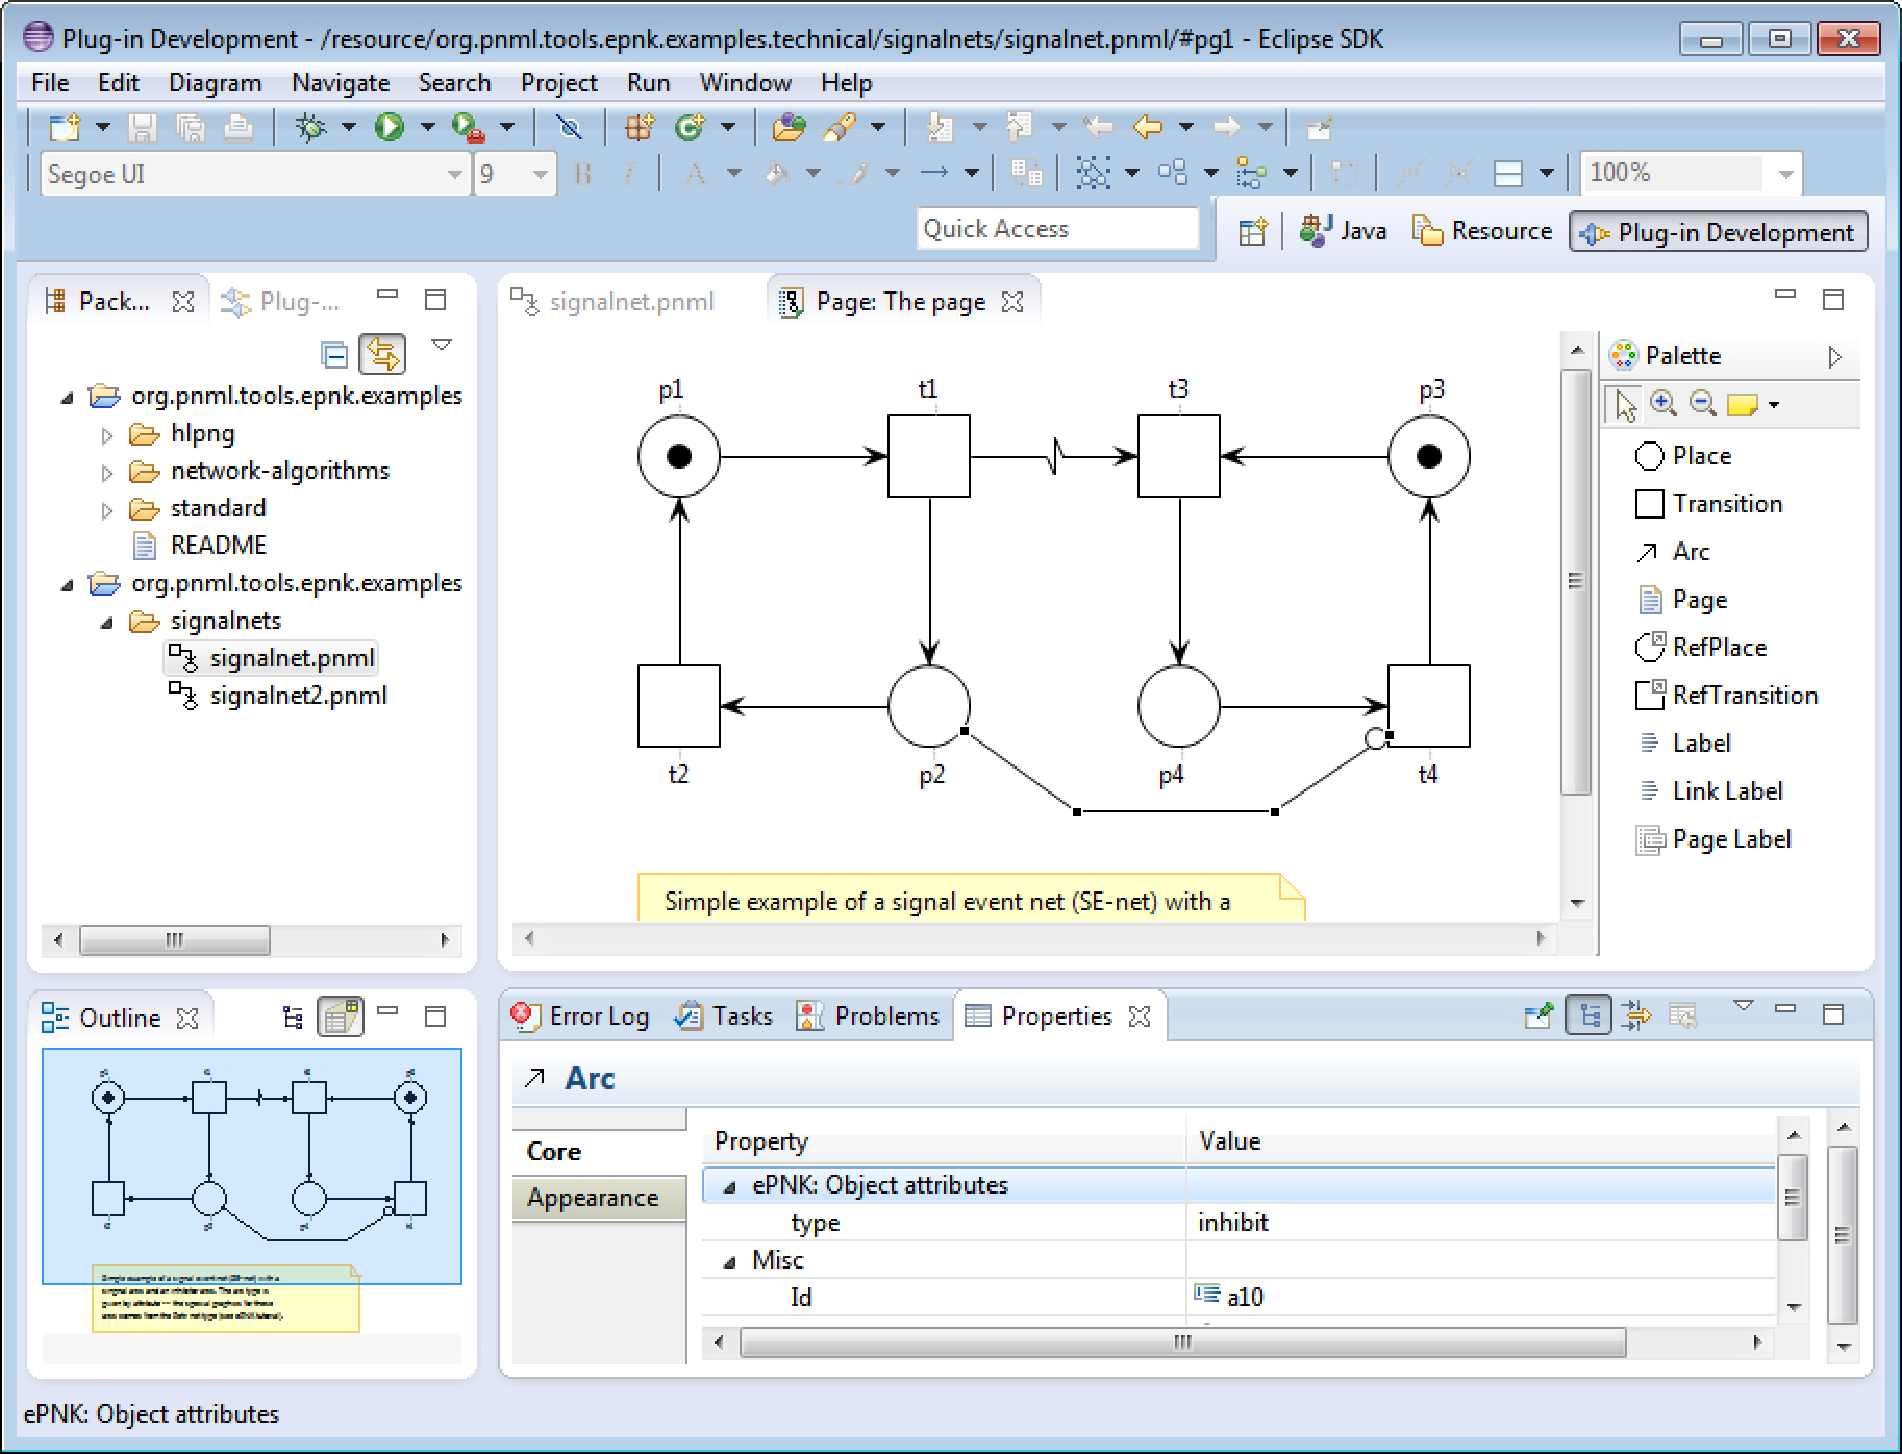
\includegraphics[scale=.38]{signalnet-attributes}}
  \caption{A SE-net with its dedicated graphics}
  \label{fig:dev:signal-net-graphics}
\end{figure}

In this section, we discuss how such dedicated graphics can be plugged
into the ePNK. To this end, we continue the discussion of the projects that
implement SE-nets, which was started in Sect.~\ref{subsec:PNTD:SE-Nets}. 
As you can see from Fig.~\ref{fig:dev:signal-net-graphics}, SE-nets have a
dedicated graphics for arcs (as signal arc, read arc, or inhibitor arc).
But there is also a dedicated graphics for places: the marking is shown
by black dots -- up to some upper bound -- in the respective places.

We start discussing the implementation of the dedicated graphical representation
for arcs. To this end, we need to implement a \emph{figure class},%
  \index{GMF!Figure class|DEF}
which is the GEF/GMF terminology for the graphically visible elements (view) of
a model element in an editor. Listing~\ref{lst:graph-ext-se-net1} shows the main
part of the class {\tt SignalnetArcFigure}, which implements the graphical appearance
of the arcs of SE-nets (the class {\tt SignalnetArcFigure} can be found in the
package {\tt org.pnml.tools.epnk.pntypes.signalnets.graphics.figures} of
plug-in project {\tt org.pnml.tools.epnk.pntypes.signalnets}).
%
\begin{figure}[htbp!]
\lstinputlisting[label=lst:graph-ext-se-net1,tabsize=2,stringstyle=\small,%
caption={The class {\tt SignalnetArcFigure}: main part}]%
{code/SignalnetArcFigure1.java}
\end{figure}
%
This class extends the class {\tt ArcFigure} of the ePNK. In line~3, an
enumeration of possible arc types is define, which is private to this class. Note that we do
not re-use the enumeration from the model here, but define another enumeration,
in order to make the implementation a bit simpler. The current type of the arc
is stored as an attribute of this class (line~5). The constructor (lines
7--11) takes the arc (the model element behind this figure) as a parameter;
it calls the constructor of the super class {\tt ArcFigure}%
  \index{ePNK!ArcFigure@{\tt ArcFigure}|DEF}
of the ePNK, which also takes the arc as a parameter, then calculates the
current type (by the private method {\tt getType()}, which is shown in
List.~\ref{lst:graph-ext-se-net2}) and then properly sets
the graphical features by calling the method {\tt setGraphics()}, which is specific to this class.

The method {\tt setGraphic()} changes the graphical features of the arc
according to the current type of the arc (lines 21--39). In this example,
we change the \emph{decorations}%
  \index{GMF!Decoration|DEF}
of the arc only; we use the decorations at both ends (source and target). As
decorations, we use the usual arrow shaped ones ({\tt
ReisigArrowHeadDecoration}\footnote {This name was chosen in honour of Wolfgang Reisig, who insisted on
   arrow heads in Petri nets being drawn in a very specific way. The
   implementation of {\tt ReisigArrowHeadDecoration} tries to meat
   Wolfgang Reisig's standards.}%
), circles ({\tt CircleDecoration}), and flashes ({\tt FlashDecoration}),
which are provided by the ePNK.%
  \index{ePNK!Arc decoration|DEF}
In the method, the variables for the decorations on both ends are initialized
to {\tt null} (lines 22-23). Then, dependent on the type of the arc the
respective decorations are set. Note that the {\tt FlashDecoration} is attached to
the source, but it will actually show up in the middle of the arc (or
actually in the middle of the first segment of the arc)  by the specific way it
is is implemented. The reason for this choice is that there can be at most
one decoration at each end of a \emph{connection}.%
  \index{GMF!Connection|DEF}
Since signal arcs have two decorations, the flash and the arrow head, one needs
to be at the source end of the connection. In the end, the only thing
that is necessary to do is actually setting the decorations -- note that calling
the respective methods with {\tt null}, means that there is no decoration for
that connection.

Note that changes in the underlying model might make changes in the
graphical appearance necessary. Such a change could be an explicit change of
the type of the arc by the end user or just reconnecting an arc to
a different kind of element. Whenever such a change happens, the ePNK
notifies the figure of the affected model element by calling
the method {\tt update()},%
  \index{ePNK!update@{\tt update()}|DEF}
which is specific to all extensible figure classes of the ePNK. It should be
overridden by the extending classes. Lines 14--19 of
List.~\ref{lst:graph-ext-se-net2} show the implementation of this method in our
example. The type of the arc is computed again; if it changed, the {\tt
setGraphics()} method is called again.

This is all there is to do for implementing another appearance of an
arc. Of course, this figure still needs to be plugged in, which is
discussed later. In the update method, you could do all kinds
of other changes such as changing the colour of the arc ({\tt
setForeGroundColor()}%
  \index{GMF!setForeGroundColor@{\tt setForeGroundColor()}|DEF}
or the line style ({\tt setLineStyle()})%
  \index{GMF!setLineStyle@{\tt setLineStyle()}|DEF}
 -- and many things more.

If you need other decorations than the ones that come with the ePNK, you can
implement them yourself. But, we do not discuss this here since this is
a GMF or, actually, an Eclipse draw2d concept. A look at the implementation of
the ePNK decorations might give you a clue.

Listing~\ref{lst:graph-ext-se-net1} shows the last part of the class {\tt
SignalnetArcFigure}: the implementation of method {\tt  getType()}. This
is mostly straightforward: computing the type based on the information
of the arc underlying this figure. The only surprise might be the
initial type check of {\tt this.arc} for {\tt Arc}. The reason is
that {\tt this.arc} refers to a final attribute of {\tt ArcFigure}
of the ePNK, which refers to the {\tt Arc} of the PNML core model,
whereas in the class {\tt SignalnetArcFigure}, we need to refer to the {\tt
Arc} of the SE-net package -- which has the same name, but in a different
package.
%
\begin{figure}[htbp!]
\lstinputlisting[label=lst:graph-ext-se-net2,tabsize=2,stringstyle=\small,%
caption={The class {\tt SignalnetArcFigure}: compute type}]%
{code/SignalnetArcFigure2.java}
\end{figure}

In the above example, we have changed the appearance of the arc on a
very high level of programming, by changing the attributes of the figure.
And if the desired graphical appearance can be achieved this way, this
is the recommended way of doing this. In some cases, however, changing
the attributes of the figure it not enough -- we rather would need to
``draw'' some additional things. This can be done by using a different
strategy for extending the figure: overriding the {\tt fillShape()}%
  \index{GMF!fillShape@{\tt fillShape()}|DEF}
or {\tt outlineShape()}
  \index{GMF!outlineShape@{\tt outlineShape()}|DEF}
methods. We explain this strategy by another example:
showing the initial marking by a respective number of black tokens in the place.
Listing~\ref{lst:graph-ext-se-place} shows the class {\tt SignalnetPlaceFigure},
which implements this graphical appearance.
%
\begin{figure}[htbp!]
\lstinputlisting[label=lst:graph-ext-se-place,tabsize=2,stringstyle=\small,%
caption={The class {\tt SignalnetPlaceFigure}}]%
{code/SignalnetPlaceFigure.java}
\end{figure}
%
The {\tt update()}%
  \index{ePNK!update@{\tt update()}|DEF}
method just informs the figure that it should repaint itself\footnote
  {We could have done that in a slightly smarter way so that
   repaint is called only if the marking has changed -- as for the arcs.}
when something has changed. The actual appearance is now defined by
overriding the method {\tt fillShape()}. In this method, first, all
the normal drawing of the place is done by calling the same method of the
{\tt super} class. After that, the marking of the place is computed\footnote
  {Since this requires some navigation in the model, this is delegated
   to a separate method {\tt getMarking()}, which is not discussed here.}%
. If the marking is between 1 and 4, the respective number of tokens
are drawn in the client area of the place. To this end, the drawing
methods on the {\tt graphics} object are used. Depending on the number of
tokens, the appropriate positions are chosen (note that for space
reasons, we omit the code for drawing four tokens). If there are more than four
tokens, they are not represented as black circles anymore. They are ``drawn'' as
a string representing the number of tokens.

Note that you could do more things and could also use some other low-level
methods of figures to do that. But, we do not discuss that here. You
might get some more inspiration my looking at another tutorial which
implements some more exotic appearances of arcs, places and transitions
in project {\tt org.pnml.tools.epnk.extensions.tutorial.types}; the
resp.\ figures can be found in the in package
{\tt org\qnsep{}pnml\qnsep{}tools\qnsep{}epnk\qnsep{}extensions\qnsep{}%
tutorial\qnsep{}types\qnsep{}arctypes\qnsep{}graphicalextensions\qnsep{}figures}.

At last we need to make the new figures defined for SE-nets known to
the ePNK -- we need to plug them in. This is done by implementing and
plugging in  a factory for these figures.
%
\begin{figure}[htbp!]
\lstinputlisting[label=lst:graph-ext-se-factory,tabsize=2,stringstyle=\small,%
caption={The factory class {\tt SignalnetGraphics}}]%
{code/SignalnetGraphics.java}
\end{figure}
%
The factory for the graphical extension for SE-nets is shown in
List.~\ref{lst:graph-ext-se-factory}. It extends the abstract ePNK
class {\tt GraphicalExtension}.%
  \index{ePNK!GraphicalExtension@{\tt GraphicalExtension}|DEF}
The first method (line 4--8) defines, for which types of Petri nets this
extension provides some graphics -- as a list of classes of the respective Petri
net types. In our example, this is the class representing SE-nets -- obtained
from the automatically generated package class. The second method (line 11--18)
defines for which kinds of elements there is a specific graphics -- again
represented as a list of class objects. In our example, these are the classes
representing the arc and the place of SE-nets. At last, there are two methods,
that create the respective figure object for an element by using the
respective constructors of the figure classes. Note that {\tt
GraphicalExtension} has also methods for creating a figure for
transitions and other kinds of nodes -- but we do not need to override them
here since our extension does not provide special graphics for them.

Actually the class {\tt GraphicalExtension} has some more methods, 
which define priorities for the graphical extensions -- in case more
than one graphical extension is plugged in and applies to the same
element. And it can also be defined, whether a graphical extension should apply
to all subtypes of a Petri net type or not.  The meaning of the methods
is documented as Java doc comments for the methods in the interface for
the factory {\tt IGraphicalExtension}.%
  \index{ePNK!IGraphicalExtension@{\tt IGraphicalExtension}|DEF}  

At last, the graphical extension needs to be plugged in to the
ePNK.  The relevant part of the ``plugin.xml'' of the project is shown
in List.~\ref{lst:graph-ext-se-plugin}. This is straightforward. The
attribute ``point'' of the extension refers to the ePNK extension
point {\tt org.pnml.tools.epnk.diagram.graphics}, and the class
attribute of the graphicsextension refers to the factory of
List.~\ref{lst:graph-ext-se-factory}.  
%
\begin{figure}[htbp!]
\lstinputlisting[label=lst:graph-ext-se-plugin,language=XML,tabsize=2,stringstyle=\small,%
caption={Plugging in the graphical extension}]%
{code/graphical-extension-se-net-plugin.xml}
\end{figure}

With this extension installed, the SE-nets should now look like the one
in Fig.~\ref{fig:dev:signal-net-graphics}.

\section{Adding tool specific information}  
\label{sec:adding-toolspecific-info}
\index{ePNK!Tool specific information|(DEF}  

As discussed in Sect.~\ref{subsec:PNMLcoremodel}, the PNML allows tool specific
information to be added to all elements of Petri nets -- indicated by the
special XML element \verb+<toolspecific>+. The ePNK reads and writes any tool
specific information, and, in principle, the contents of these tool
specific extensions could be accessed and modified via the class {\tt AnyType},
which is defined in the plug-in {\tt org.eclipse.emf.ecore}. But this
is tedious and, basically, means navigating in the element's XML structure.

Therefore, the ePNK provides an extension point for plugging in tool specific
extensions, so that they can be accessed and modified via an API specific to the
extension which can be defined in terms of a model. We will discuss how to
use this extension point by the help of an example: the token positions, which
is a tool specific extension mandated by ISO/IEC~15909-2:2011. We have seen an
example already in Fig.~\ref{fig:sample-net} and Listing~\ref{lst:sample-net} on
page~\pageref{lst:sample-net}.

This tool specific extension is defined in the project
{\tt org\qnsep{}pnml\qnsep{}tools\qnsep{}epnk\qnsep{}toolspecific\qnsep{}tokenpositions}.
Most of this code in this project as well as the ``plugin.xml'' was
automatically generated by EMF from the Ecore model ``Tokenpositions.ecore''
in the folder ``model''. This model is shown in Fig.~\ref
{fig:ToolSpecificTokenPosModel}.
%
\begin{figure}[hbt!!]
  \centerline{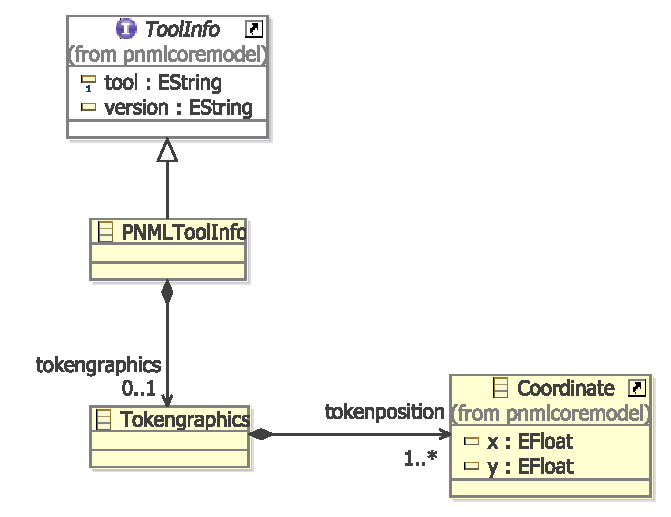
\includegraphics[scale=.60]{Tokenpositions}}
  \caption{The model for tool specific extension tokenpositions}
  \label{fig:ToolSpecificTokenPosModel}
\end{figure}
%
The new classes are {\tt PNMLToolInfo} and {\tt Tokengraphics}. The class 
{\tt PNMLToolInfo} represents the actual tool specific information: it must
implement the PNML core model interface {\tt ToolInfo}.%
  \index{ePNK!ToolInfo@{\tt ToolInfo}|DEF}
The actual contents of this tool specific information is {\tt Tokengraphics},
which consists of one or many coordinates; the class {\tt Coordinate} is
re-used from the PNML core model. 

From this model, the code can be generated in the same way as described in
Sect.~\ref{subsubsec:type-codegeneration}. First, the ``genmodel'' must be
created, and from the ``genmodel'', the model code and the edit code must be
generated.

After the code generation, the only thing left to do is to manually create a
factory for this tool specific extension, and use this factory for plugging
it into the ePNK. The factory for our extension is shown in
Listing~\ref{lst:tool-spec-extension-factory}.
%
\begin{figure}[htbp!]
\lstinputlisting[label=lst:tool-spec-extension-factory,tabsize=2,stringstyle=\small,%
caption={Factory for the tool specific extension}]%
{code/TokenpositionsExtensionFactory.java}
\end{figure}
%
The factory implements the ePNK interface {\tt ToolspecificExtensionFactory},%
  \index{ePNK!ToolspecificExtensionFactory@{\tt ToolspecificExtension
    Factory}|DEF}
which consists of four methods. The two methods {\tt createToolInfo()}%
  \index{ePNK!createToolInfo@{\tt createToolInfo()}|DEF}
create an instance of this tool specific extension; the method with the two
String parameters, {\tt tool} and {\tt version} is used, when the tool
name and version are given, which might return instances of different classes --
in our example, however, the version number is irrelevant. The two other
methods, must return the tool name for that extension and its version, which, in
our example, are encoded as constants.

Listing~\ref{lst:tokenpositions-plugin} shows the fragment of the ``plugin.xml''
that is needed to plug in the token position extensions to the ePNK. In
addition to the name and the id, there is an attribute {\tt class}
that defines the factory for the tool specific extension; this class must
implement the interface {\tt Toolspecific\optsep{}ExtensionFactory}.
%
\begin{figure}[htbp!]
\lstinputlisting[label=lst:tokenpositions-plugin,language=XML,tabsize=2,stringstyle=\small,%
 caption={Plugging in the token position extension}]%
{code/tokenpositions-plugin.xml}
\end{figure}
%
Moreover, there is a brief description of this extension. 

Note that the ePNK does not provide any way yet of explicitly defining the XML
syntax of these extensions. The standard XMI serialisation will be used --
which is compliant with ISO/IEC~15909-2:2011 for tool specific extensions.
Eventually, the ePNK might provide a mapping mechanism similar to the one
for Petri net types.%
  \index{ePNK!Tool specific information|)}

\section{Overview of the ePNK and its projects}
\label{sec:overviewAPI}

In this section, we give a brief overview of the different parts of the ePNK,
the project structure and where to look for different kinds of functionality in
the ePNK API an its projects. As mentioned earlier, developers should not change
anything in these projects. Anyway, this overview should help to better understand the ideas
behind the ePNK, the necessary dependencies (that need to be included in
new projects via the  ``plugin.xml'') and the functions that are available in
the ePNK API, which could be used by developers in their extensions. Note that
we do not discuss the details of the API here. In particular, we do
not discuss the API concerning the code that is generated from the Ecore
models (model and edit code) since it is mostly straightforward.
Section~\ref{subsubsec:ePNK:API:EMF} gives a brief overview of the main
principles behind the model code that is generated from Ecore models; for
more information, we refer to the EMF book \cite{BSM06}.

Like all extensions of Eclipse, the ePNK is organized in many Eclipse projects,
which together make the ePNK. Most of these projects are so-called plug-in
projects; and these are the ones most relevant for developers, since
these are the projects to look up the API and to which extensions need to
refer (in form of dependencies). In addition, there are some projects, which
contain documentation only (like this manual), there are some projects that
do not contain any code, but from which other projects are generated; and
there are so-called features, which define collections of plug-in projects in
order to deploy them. And there is a project for generating the ePNK update site
from the features.

In this manual, we focus on the plug-in projects of the ePNK, the most important
of which are listed below. We start with an overview of the ePNK core projects,
which make up the framework of the ePNK\footnote
  {Technically, all these plug-in projects are part of the ePNK features
   {\tt org.pnml.tools. epnk.core}  and
   {\tt org.pnml.tools.epnk.extensions.basic}.}%
:
\begin{description}
  \item[{\tt org.pnml.tools.epnk}:] ~\\
  This is the core project of the ePNK. In
  this project, you will find the PNML core model, some additional models, and the
    \emph{model code}, that was generated from them. All the models, can be
    found in the folder ``model''. The PNML core model is contained in
    {\tt PNMLCoreModel\qnsep{}ecore};%
        \index{PNML Core Model|DEF}
    in order to avoid clutter in the graphical
    diagram, the core model is actually split up into three separate diagrams:
    {\tt PNMLCore\optsep{}Model\qnsep{}ecorediag} contains the most important
    concepts; {\tt PNMLCore\optsep{}Model\optsep{}Graphics\qnsep{}ecorediag}
    contains the graphical features of PNML; and {\tt PNMLCoreModelProxies\qnsep{}ecorediag} contains some extensions
    to the PNML core model that are necessary to maintain labels in the
    graphical editor of the ePNK by so-called \emph{label proxies}%
      \index{ePNK!Label proxy|DEF}
    and \emph{page label proxies}.%
      \index{ePNK!Page label proxy|DEF}
   These proxy elements, however, are not of any concern for normal developers.

    There are four other models in this project: {\tt PNMLDataTypes.ecore}
    defines the \emph{data types}%
       \index{ePNK!Data types|DEF}
    for non-negative and positive numbers, which are used instead of the
    respective XML Schema Data Types of ISO/IEC 15909-2. {\tt
    PNMLStructuredPNTypeModel\qnsep{}ecore} defines the concepts of structured
    Petri net types%
      \index{ePNK!structured Petri net type|DEF}
    (see Sect.~\ref{subsubsec:structuredPNTs}).
    {\tt Serialisation\qnsep{}ecore} provides some general structure that is
    used for the XML serialisation of so-called association elements%
      \index{ePNK!Association element|DEF}
    (see Sect.~\ref{subsubsec:XMLmapping}).
    {\tt PNMLPageDiagram\optsep{}Info\qnsep{}ecore} is the model for storing the
    GMF diagram information%
      \index{ePNK!Diagram information|DEF}
    for pages as ePNK tool specific information in PNML models, which are not of
    concern for normal developers.
    
    This project provides also some \emph{convenience classes}%
      \index{ePNK!Convenience classes|DEF}
    in package {\tt org\qnsep{}pmm\qnsep{}tools\qnsep{}epnk\qnsep{}helpers},
    which might be helpful in practice. The class {\tt FlatAccess}%
      \index{ePNK!FlatAccess@{\tt FlatAccess}|DEF}
    allows handling a Petri net that is
    distributed over several pages as if it was flat (see
    Sect.~\ref{subsec:tutorial-MC} for an example).
    Another convenience class is {\tt NetFunctions},%
      \index{ePNK!NetFunctions@{\tt NetFunctions}|DEF}
    which provides many static methods for finding out to which net an element
    belongs, what the type of this net is, and for obtaining lists of
    elements of some kind of a given Petri net.
    
    In this plug-in, also the two extension points of the ePNK are defined:
    one for defining new Petri net types (PNTD), another for defining 
    new tool specific extensions.%
      \index{ePNK!PNTD}%
      \index{ePNK!Tool specific extension}
    
    In addition to the model code, also the so-called edit code and editor
    code are generated from these models, which together define the tree
    editor for PNML (see below).
    
    Note that, in this project, also the constraint context and the
    constraint category {\tt org\qnsep{}pnml\qnsep{}tools\qnsep{}epnk\qnsep{}validation},%
      \index{ePNK!Validation}%
      \index{ePNK!Constraints|DEF}
    to which all other constraints for new Petri net types should be added, are
    defined here (see Sect.~\ref{subsubsec:simplePNTDconstraints}
    and~\ref{subsubsec:PNTDConstraints}).
    
  \item[{\tt org.pnml.tools.epnk.edit}:] ~\\
    This project contains the edit code
    that was generated from the models in project {\tt org.pnml.tools.epnk}.
    Though most of this code was automatically generated from the models,
    there are several manual changes, that enable generically dealing with
    plugged in Petri net type definitions.
    
    Moreover, the generated standard EMF images in the folder {\tt icons}
    were replaced by nicer ones.
    
  \item[{\tt org.pnml.tools.epnk.editor}:] ~\\
    This project contains the editor
    code for the EMF tree editor for PNML that was generated from the models in
    project {\tt org\qnsep{}pnml\qnsep{}tools\qnsep{}epnk}. In this project,
    there are only a few, but crucial extensions, that made it possible to
    integrate the EMF tree editor with the graphical editor for pages (see the
    plug-in project
    {\tt org\qnsep{}pnml\qnsep{}tools\qnsep{}epnk\qnsep{}diagram} below).
              
  \item[{\tt org.pnml.tools.epnk.pntypes}:] ~\\
    This project contains the model
    and the generated model code for P/T-nets ({\tt PTNet}),%
        \index{ePNK!PTNet@{\tt PTNet}}
    as well as the extension that plugs in this type to the ePNK. The model code
    is completely generated from the model {\tt PTNet.ecore} in the folder
    ``model'', except for two changes in class {\tt PTNetImpl} as discussed in
    Sect.~\ref{subsec:simplePNTD}.

  \item[{\tt org.pnml.tools.epnk.pntypes.edit}:] ~\\
    This is the project with the
    edit code that was generated from the Ecore model {\tt PTnet\qnsep{}ecore}
    of project {\tt org\qnsep{}pnml\qnsep{}tools\qnsep{}epnk\qnsep{}pntypes}.
    There are no manual changes in the generated code -- only the icons in the
    folder {\tt icons} were replaced by nicer ones.
    
  \item[{\tt org.pnml.tools.epnk.toolspecific.tokenpositions}:] ~\\
    In this project,
    the tool specific extension for token positions%
        \index{Token positions|DEF}
    (as defined in ISO/IEC~15909-2) is defined (see
    Sect.~\ref{sec:adding-toolspecific-info}). The model code and the edit
    project {\tt org.pnml.tools.epnk.toolspecific.token\-po\-si\-tions.edit}
    was generated (which does not contain any manual changes -- not even nicer icons) from the model
    {\tt Tokenposition.ecore}.

    Note that the ePNK does not take the information of these token positions
    into account in the graphical representation of places. The only reason they
    are defined in the ePNK is that ISO/IEC~15909-2:2011 mandates them
    -- and we use this extension as an example to show how to define tool specific
    extensions in Sect.~\ref{sec:adding-toolspecific-info}.
    
  \item[{\tt org.pnml.tools.epnk.actions}:] ~\\
    This project defines the
    standard actions of the ePNK, which are the pop-up menus for adding
    missing ids and for linking the labels of structured Petri net types
    (see Sect.~\ref{subsubsec:structuredPNTs}).
    
    Moreover, the classes {\tt AbstractEPNKAction}%
        \index{ePNK!AbstractEPNKAction@{\tt AbstractEPNKAction}|DEF}
    and {\tt AbstractEPNKJob}% 
         \index{ePNK!AbstractEPNKJob@{\tt AbstractEPNKJob}|DEF}
    are defined in this project, which are convenience classes to make it easier
    to define functions for the ePNK that run in the background (see
    Sect.~\ref{subsec:tutorial-MC}).
    
  \item[{\tt org.pnml.tools.epnk.diagram}:] ~\\
    This project contains the code for
    the GMF-generated graphical editor for pages of Petri nets. This code was
    generated from the GMF models in project {\tt org.pnml.tools.epnk.gmf}.
    But, there are major manual changes for making this graphical editor
    generic and for integrating it with the tree editor for PNML (see
    project {\tt org\qnsep{}pnml\qnsep{}tools\qnsep{}epnk\qnsep{}editor}).
    
    The package {\tt org.pnml.tools.epnk.gmf.extensions.graphics} and its%
      \index{ePNK!Customizing graphics|DEF}
    sub-packages {\tt decorations}%
      \index{ePNK!Decorations|DEF}
    and {\tt figures}%
      \index{ePNK!Figures|DEF}
    are relevant for 
    developers, who want to contribute specific graphical appearances for
    some Petri nets. Here you find the factory and the figures of the ePNK,
    which need to be extended for customizing the graphical appearance;
    and you can use the predefined ePNK decorations for that purpose
    (see Sect.~\ref{sec:dev:graphical} for more details). 
    
  \item[{\tt org.pnml.tools.epnk.gmf.integration}:] ~\\
    This project defines the
    pop-up menus for starting the graphical editor on a page that is selected in
    a tree editor or in a graphical editor.
    
  \item[{\tt org.pnml.tools.epnk.annotations}:] ~\\
    This project defines the
    infrastructure for annotating Petri nets by applications. Up to now,
    the annotations%
        \index{ePNK!Annotation|DEF}
    provide the most basic concepts only -- they will be extended in the
    future.

    A simple example of annotating the context of transitions was discussed
    in Sect.~\ref{subsec:developer:applications}.
    
  \item[{\tt org.pnml.tools.epnk.applications}:] ~\\
    This project provides the
    interfaces and classes for implementing and starting applications on Petri
    nets, which was briefly discussed in
    Sect.~\ref{subsec:developer:applications}.%
       \index{ePNK!Application|DEF}
    
  \item[{\tt org.pnml.tools.epnk.applications.view}:] ~\\
    This project implements
    the applications view, that shows all currently running implementations.
    Developers would typically not directly use this project. 
\end{description}

Next, we discuss some of the net types, and functions and applications, which we
had discussed in this manual as a tutorial\footnote
  {Technically, these plug-in projects come from the ePNK feature
   {\tt org.pnml.tools. epnk.extensions.tutorial}.}%
:
\begin{description}
  \item[{\tt org.pnml.tools.epnk.functions.tutorials}:] ~\\
    This project contains the functions that were discussed in
    Sect.~\ref{subsec:file-overview} and Sect.~\ref{subsect:multi-agent},
    which can serve as a guideline for defining own extension projects.
    
  \item[{\tt org.pnml.tools.epnk.functions.modelchecking}:] ~\\
     This project
     contains the model checker extension%
          \index{Model checker}
     for the ePNK that is discussed in Sect.~\ref{subsec:tutorial-MC}. Note that
     the project {\tt MCiE} is used in this model checker extension only (MCiE
     is not relevant for anything else in the ePNK -- except if you want to
     implement your own model checker based on MCiE).

 \item[{\tt
 org\qnsep{}pnml\qnsep{}tools\qnsep{}epnk\qnsep{}tutorials\qnsep{}applications}:]  ~\\
    This project implements an example of an application%
      \index{ePNK!Application}
    using annotations.%
        \index{ePNK!Annotation|DEF}
    It contains the code for the transition context application which was
    discussed in Sect.~\ref{subsec:developer:applications}.
    
 \item[{\tt org.pnml.tools.epnk.pntypes.signalnets}:] ~\\
    This project is 
    the plug-in project implementing the Petri net type definition for SE-nets%
      \index{SE-nets|DEF}
    (see Sect.~\ref{subsec:PNTD:SE-Nets} and the graphical extensions for
    SE-nets (see Sect.~\ref{sec:dev:graphical}).

\item[{\tt org.pnml.tools.epnk.pntypes.signalnets.edit}:] ~\\
    This plug-in project
    contains the edit code, which is generated from the model of SE-nets
    -- without any manual changes      
\end{description}

The plug-in projects with the prefix {\tt org\qnsep{}pnml\qnsep{}tools\qnsep{}epnk\qnsep{}pntypes\qnsep{}hlpng}
resp.\ {\tt org\qnsep{}pnml\qnsep{}tools\qnsep{}epnk\qnsep{}pntypes\qnsep{}hlpngs} together are used for defining
high-level Petri nets (HLPNGs).%
  \index{ePNK!HLPNG|(DEF}
The following list gives an overview in a bottom
up way -- ending with the actual Petri net type definition for HLPNGs:

\begin{description}
\item[{\tt org.pnml.tools.epnk.pntypes.hlpngs.datatypes}:] ~\\
   In this project, all
   the models that define the concepts of sorts, operators, variables and terms
   for HLPNGs are contained. In particular, there is a model  {\tt
   HLPNGDataTypes.ecore} for the general structure of terms, declarations
   and the built-in sorts and operators that occur in all versions of HLPNGs.
   And there are many more models and diagrams for specific versions of
   HLPNGs (Clauses~5.3.2--5.3.12 of ISO/IEC~15909-2:2011).
 
\item[{\tt org.pnml.tools.epnk.pntypes.hlpngs.datatypes.concretesyntax}:] ~\\
   This project is an Xtext project that defines the grammar for the concrete
   syntax of the different labels of HLPNGs, from which a parser is generated.
   Here, we do not discuss the details of generating the parser. The manually written
   class {\tt HLPNGParser} accesses the automatically generated parsing
   operations and provides methods for parsing every
   kind of label of HLPNGs. The other important manually written class is
   {\tt HLPNGLinker}, which provides the global Linker for labels (as discussed
   in Sect.~\ref{subsubsec:structuredPNTs}).

   Note that the plug-in project ending with 
   {\tt concretesyntax\qnsep{}ui} was
   automatically created when the Xtext project was created by a wizard;
   it provides a stand-alone textual editor for the labels of HLPNGs.
   Since this stand-alone editor is not needed for the ePNK, this project is
   not part of the standard deployment of the ePNK. 

\item[{\tt org.pnml.tools.epnk.pntypes.hlpng.pntd}:] ~\\
   This project actually
   combines all the parts discussed above into a Petri net type definition for
   HLPNGs. The main model is {\tt HLPNG\optsep{}Definition.ecore}, which was
   shown in Fig.~\ref{fig:HLPNG-Terms}. The other model {\tt
   HLPNGSerialisation.ecore} defines the auxiliary classes that temporarily
   store XML elements that represent associations and are used and referred to
   in the XML mappings (see Sect.~\ref{subsubsec:XMLmapping}) .
   
   The global linker {\tt HLPNGLinker} from the project 
   {\tt org\qnsep{}pnml\qnsep{}tools\qnsep{}epnk\qnsep{}pntypes\qnsep{}hlpngs\qnsep{}datatypes\qnsep{}concretesyntax}
   above is made available in the Petri net type by
   manually implementing the method {\tt getLinker()} in class {\tt HLPNGImpl}.
   The {\tt parse()} method for the different structured labels are also
   manually implemented -- they refer to the different {\tt parserXXX()} methods
   of class {\tt HLPNGParser}%
     \index{ePNK!HLPNG|)}
   from the project
   {\tt org\qnsep{}pnml\qnsep{}tools\qnsep{}epnk\qnsep{}pntypes\qnsep{}hlpngs\qnsep{}datatypes\qnsep{}concretesyntax}
   above.
   
\item[{\tt org.pnml.tools.epnk.helpers.unparse}:] ~\\
   This project implements
   a serialisation function that transforms the abstract syntax of
   HLPNG labels into the concrete syntax used for HLPNGs in the ePNK.
   This is mostly relevant for the end users -- who want to generate
   the concrete syntax for the labels of HLPNGs (see
   Sect.~\ref{sec:user:hlpng:label-serialisation} on
   page~\pageref{sec:user:hlpng:label-serialisation}).
   
   But, in some cases this label serialiser might also be relevant
   for developers that want to show terms of HLPNGs to the end user
   (the simulator for high-level nets is an example). 
   
\item[{\tt org.pnml.tools.epnk.applications.hlpng.simulator}:] ~\\
   This is the
   plug-in project implementing the basic simulator for HLPNGs. We do not
   discuss the implementation in this manual, we discussed the simulator only
   from the end users' point of view in Sect.~\ref{subsec:user:hlpng-simulator}.
   You will find many more details in the master's thesis that implemented it
   \cite{Lag12}.
\end{description}

\section{Deploying extensions}
\label{sec:developer:deploy}  

In this section, we will briefly discuss how own extensions of the ePNK could
be deployed, so that others can use it. Typically, an extension comprises
several plug-in projects. In order to combine them, Eclipse provides a special
kind of project, which is called a \emph{feature}%
  \index{Eclipse!Feature|DEF}
-- and this is the unit in which Eclipse extensions should be deployed. 


A feature in turn, can be used in an Eclipse \emph{update site project}%
  \index{Eclipse!Update site|DEF}
which can be used to create your own \emph{update site}, so that your plug-ins
(resp.\ features) could be installed from this site, similar to the way you
installed the ePNK.

Since features and update sites are standard Eclipse concepts, we
do not explain the details here. For now, looking up the keywords ``feature''
and ``update site'' in the Eclipse help (or googling for them) should be
enough.

If you have a feature for the ePNK that might be interesting for a wider
audience, you can also contact us, so that we can make it available via the
ePNK update site.
